% chapter.tex (Chapter 02)
\chapter{কমিউনিকেশন সিস্টেমস ও নেটওয়ার্কিং}

\begin{learningbox}
এই অধ্যায় শেষে শিক্ষার্থী পারবে:
\begin{itemize}
\item ডেটা কমিউনিকেশন সিস্টেমের উপাদান, ব্যান্ডউইডথ এবং সিগন্যাল ব্যাখ্যা করতে।
\item ডেটা ট্রান্সমিশন মেথড, মোড এবং কমিউনিকেশন মিডিয়ার শ্রেণিবিভাগ করতে।
\item তারযুক্ত ও তারবিহীন মাধ্যমের ব্যবহার, সুবিধা ও সীমাবদ্ধতা তুলনা করতে।
\item মোবাইল কমিউনিকেশন, কম্পিউটার নেটওয়ার্ক, নেটওয়ার্ক ডিভাইস ও টপোলজি বিশ্লেষণ করতে।
\item ক্লাউড কম্পিউটিংয়ের ধারণা, সেবা মডেল এবং বাস্তব ব্যবহার ব্যাখ্যা করতে।
\end{itemize}
\end{learningbox}

\begin{keypointbox}{এই অধ্যায় কেন গুরুত্বপূর্ণ}
আমরা প্রতিদিন mobile phone, Wi-Fi, online class, social media, cloud storage, online payment এবং internet ব্যবহার করি। এগুলোর পেছনে মূল ভিত্তি হলো data communication, transmission media, network device, topology এবং cloud computing। তাই এই অধ্যায় শুধু পরীক্ষার জন্য নয়, বাস্তব ICT বুঝতেও খুব গুরুত্বপূর্ণ।
\end{keypointbox}

\begin{figure}[H]
\centering
\fbox{
\parbox{0.92\textwidth}{
\centering
Communication System\\[4pt]
$\downarrow$\\[4pt]
Data Transmission\\[4pt]
$\downarrow$\\[4pt]
Transmission Media\\[4pt]
$\downarrow$\\[4pt]
Mobile Communication\\[4pt]
$\downarrow$\\[4pt]
Computer Network\\[4pt]
$\downarrow$\\[4pt]
Network Devices \quad Topology\\[4pt]
$\downarrow$\\[4pt]
Cloud Computing
}}
\caption{দ্বিতীয় অধ্যায়ের ধারণা মানচিত্র}
\end{figure}

\begin{keypointbox}{High-yield অংশ}
\begin{itemize}
\item কমিউনিকেশন সিস্টেম: Sender, Receiver, Message, Medium, Protocol।
\item ব্যান্ডউইডথ: bps, Kbps, Mbps, Gbps; Narrow band, Voice band, Broadband।
\item ট্রান্সমিশন মেথড: Parallel, Serial; Serial-এর মধ্যে Asynchronous, Synchronous, Isochronous।
\item ট্রান্সমিশন মোড: Simplex, Half duplex, Full duplex।
\item ডেলিভারি মোড: Unicast, Broadcast, Multicast।
\item মিডিয়া: Guided/Wired এবং Unguided/Wireless।
\item নেটওয়ার্ক: PAN, LAN, CAN, MAN, WAN।
\item টপোলজি: Bus, Ring, Star, Tree, Mesh, Hybrid।
\item ক্লাউড কম্পিউটিং: IaaS, PaaS, SaaS; Public, Private, Hybrid, Community cloud।
\end{itemize}
\end{keypointbox}

\begin{boardbox}{বোর্ড ও ভর্তি পরীক্ষার জন্য নির্দেশনা}
এই অধ্যায়ে diagram, comparison table এবং বাস্তব উদাহরণ খুব গুরুত্বপূর্ণ। সংজ্ঞা মুখস্থ করার পাশাপাশি প্রতিটি term কোথায় ব্যবহার হয় তা বুঝতে হবে। বিশেষ করে bandwidth calculation, transmission mode, media comparison, network device এবং topology থেকে MCQ ও CQ বেশি হওয়ার সম্ভাবনা থাকে।
\end{boardbox}

% Chapter 02.1: কমিউনিকেশন সিস্টেম ও ব্যান্ডউইডথ
\section{কমিউনিকেশন সিস্টেম ও ব্যান্ডউইডথ}

\subsection{কমিউনিকেশন সিস্টেমের ধারণা}

\begin{itemize}
\item কমিউনিকেশন কী
\item কমিউনিকেশন সিস্টেম কী
\item তথ্য প্রেরণ ও গ্রহণের ধারণা
\item ডেটা ও সিগন্যালের সম্পর্ক
\item Analog signal ও Digital signal
\end{itemize}

\subsection{কমিউনিকেশন মডেল}

\begin{itemize}
\item Source System
\item Transmitter
\item Transmission System / Medium
\item Receiver
\item Destination System
\end{itemize}

\subsection{ডেটা কমিউনিকেশনের ধারণা}

\begin{itemize}
\item Data communication কী
\item ডেটা প্রেরণ ও গ্রহণ
\item ডেটা কমিউনিকেশনের প্রয়োজনীয়তা
\item Sender / Source, Receiver / Destination, Medium, Message, Protocol
\end{itemize}

\subsection{ব্যান্ডউইডথ}

\begin{itemize}
\item ব্যান্ডউইডথের ধারণা
\item ডেটা প্রেরণের ক্ষমতা
\item bps, Kbps, Mbps, Gbps
\item Narrow Band, Voice Band, Broadband
\end{itemize}

% Chapter 02.2: ডেটা ট্রান্সমিশন মেথড ও ডেটা ট্রান্সমিশন মোড
\section{ডেটা ট্রান্সমিশন মেথড ও মোড}

\begin{learningbox}
এই টপিক শেষে শিক্ষার্থী পারবে:
\begin{itemize}
\item asynchronous, synchronous ও isochronous transmission ব্যাখ্যা করতে।
\item start bit, stop bit ও clock synchronization-এর ভূমিকা বুঝতে।
\item simplex, half duplex ও full duplex mode আলাদা করতে।
\item একটি table বা tree ব্যবহার করে transmission method compare করতে।
\item board-style comparison question-এর উত্তর লিখতে।
\end{itemize}
\end{learningbox}

\subsection{ডেটা ট্রান্সমিশন মেথড}
\subsubsection{Asynchronous Transmission}
\begin{itemize}
\item Start bit, Stop bit
\item Character by character transmission
\item ব্যবহার-বর্ণনা, সুবিধা ও অসুবিধা
\end{itemize}

\subsubsection{Synchronous Transmission}
\begin{itemize}
\item Block by block transmission
\item Clock synchronization
\item উচ্চ গতির ডেটা প্রেরণ
\end{itemize}

\subsubsection{Isochronous Transmission}
\begin{itemize}
\item Real-time audio/video transmission
\item Multimedia communication-এ ব্যবহার
\end{itemize}

\subsection{ডেটা ট্রান্সমিশন মোড}
\subsubsection{Simplex}
\begin{itemize}\item একমুখী ডেটা প্রেরণ; উদাহরণ: TV broadcasting\end{itemize}
\subsubsection{Half Duplex}
\begin{itemize}\item উভয় দিকে ডেটা যায়, কিন্তু একই সময়ে নয়; উদাহরণ: walkie-talkie\end{itemize}
\subsubsection{Full Duplex}
\begin{itemize}\item একই সময়ে উভয় দিকে data আদান-প্রদান; উদাহরণ: telephone\end{itemize}

\subsection{ডেটা ট্রান্সমিশন মোড}

\begin{definitionbox}{ডেটা ট্রান্সমিশন মোড}
ডেটা প্রেরণ ও গ্রহণের দিক এবং একই সময়ে data flow-এর মাত্রাকে transmission mode বলা হয়।
\end{definitionbox}

\subsubsection{Simplex}

Simplex mode-এ data শুধু একদিকে যায়। Receiver কোনো data ফেরত পাঠায় না।

\begin{definitionbox}{সিম্প্লেক্স}
যে transmission mode-এ data কেবল একদিকে প্রেরিত হয়, তাকে simplex mode বলে।
\end{definitionbox}

\begin{examplebox}{উদাহরণ}
TV broadcasting, radio broadcasting এবং digital notice board simplex-এর সহজ উদাহরণ।
\end{examplebox}

\subsubsection{Half Duplex}

Half duplex mode-এ দুই দিকেই data যেতে পারে, কিন্তু একই সময়ে নয়। এক পক্ষ কথা বললে অন্য পক্ষ শুনে।

\begin{definitionbox}{হাফ ডুপ্লেক্স}
যে transmission mode-এ উভয় দিকে data আদান-প্রদান সম্ভব, কিন্তু একই সময়ে নয়, তাকে half duplex বলে।
\end{definitionbox}

\begin{examplebox}{উদাহরণ}
Walkie-talkie, old-style intercom এবং কিছু shared channel communication half duplex-এর উদাহরণ।
\end{examplebox}

\subsubsection{Full Duplex}

Full duplex mode-এ একই সময়ে উভয় দিকে data আদান-প্রদান হয়। এটি সবচেয়ে কার্যকর এবং স্বাভাবিক conversation-like communication-এর জন্য উপযুক্ত।

\begin{definitionbox}{ফুল ডুপ্লেক্স}
যে transmission mode-এ উভয় দিকেই একই সময়ে data প্রেরণ ও গ্রহণ করা যায়, তাকে full duplex বলে।
\end{definitionbox}

\begin{examplebox}{উদাহরণ}
Telephone call, video chat, modern internet communication এবং two-way live conferencing full duplex-এর উদাহরণ।
\end{examplebox}

\begin{center}
\begin{tabular}{|p{0.22\textwidth}|p{0.22\textwidth}|p{0.22\textwidth}|p{0.22\textwidth}|}
\hline
\textbf{Mode} & \textbf{Direction} & \textbf{Same time?} & \textbf{উদাহরণ} \\
\hline
Simplex & একদিকে & না & TV broadcasting \\
\hline
Half duplex & দুইদিকে & না & Walkie-talkie \\
\hline
Full duplex & দুইদিকে & হ্যাঁ & Telephone \\
\hline
\end{tabular}
\end{center}

\begin{boardbox}{বোর্ড ফোকাস}
Transmission method-এর প্রশ্নে method ও mode গুলোর পার্থক্য খুব পরিষ্কার করে লিখতে হয়। Table, example এবং এক লাইনের conclusion দিলে answer strong হয়।
\end{boardbox}

\begin{recapbox}
\begin{itemize}
\item Asynchronous-এ প্রতিটি character আলাদা, synchronous-এ বড় block, isochronous-এ নির্দিষ্ট সময়ভিত্তিক data যায়।
\item Simplex একদিকে, half duplex দুইদিকে কিন্তু একই সময়ে নয়, full duplex দুইদিকে একই সময়ে।
\item Real-time media-এর জন্য isochronous খুব গুরুত্বপূর্ণ।
\item পরীক্ষায় compare table আঁকলে উত্তর দ্রুত বোঝা যায়।
\end{itemize}
\end{recapbox}

\begin{practicebox}
\textbf{MCQ}
\begin{enumerate}
\item Start bit ও stop bit কোন transmission method-এ ব্যবহৃত হয়?\\
ক. Synchronous \quad খ. Asynchronous \quad গ. Isochronous \quad ঘ. Full duplex
\item একই সময়ে উভয় দিকে data আদান-প্রদান কোন mode-এ সম্ভব?\\
ক. Simplex \quad খ. Half duplex \quad গ. Full duplex \quad ঘ. Broadcast
\end{enumerate}

\textbf{সংক্ষিপ্ত প্রশ্ন}
\begin{enumerate}
\item Asynchronous ও synchronous transmission-এর মধ্যে দুটি পার্থক্য লেখ।
\item Half duplex mode-এর একটি বাস্তব উদাহরণ দাও।
\end{enumerate}

\textbf{সৃজনশীল অনুশীলন}
একটি online class-এ শিক্ষক ভিডিও, audio ও slide একসঙ্গে পাঠাচ্ছেন; আবার শিক্ষার্থীরা প্রশ্ন পাঠাচ্ছে। উদ্দীপকের আলোকে transmission method ও mode বিশ্লেষণ করো।
\end{practicebox}


\subsection{শ্রেণিবিন্যাস ও চিত্র}

\begin{center}
\fbox{\parbox{0.92\textwidth}{
\centering
\textbf{Tree diagram placeholder: Data Transmission}\\[4pt]
Data Transmission\\
$\rightarrow$ Method: Parallel, Serial\\
$\rightarrow$ Serial Synchronization: Asynchronous, Synchronous, Isochronous\\
$\rightarrow$ Direction Mode: Simplex, Half Duplex, Full Duplex\\
$\rightarrow$ Receiver-based Mode: Unicast, Broadcast, Multicast
}}
\end{center}

\begin{definitionbox}{Parallel transmission}
যে পদ্ধতিতে একটি character বা data word-এর একাধিক bit একই সময়ে একাধিক line দিয়ে গন্তব্যে পাঠানো হয়, তাকে parallel transmission বলা হয়। এটি কাছাকাছি ডিভাইসের জন্য দ্রুত হলেও বেশি line দরকার হয়।
\end{definitionbox}

\begin{definitionbox}{Serial transmission}
যে পদ্ধতিতে bit-গুলো একটির পর একটি ধারাবাহিকভাবে একটি channel দিয়ে পাঠানো হয়, তাকে serial transmission বলা হয়। দূরবর্তী যোগাযোগে এটি বেশি ব্যবহারযোগ্য।
\end{definitionbox}

\begin{center}
\begin{tabular}{|p{0.22\textwidth}|p{0.34\textwidth}|p{0.34\textwidth}|}
\hline
\textbf{ভিত্তি} & \textbf{Parallel} & \textbf{Serial} \\
\hline
Bit flow & একসাথে একাধিক bit & একটির পর একটি bit \\
\hline
দূরত্ব & কম দূরত্বে সুবিধাজনক & বেশি দূরত্বে সুবিধাজনক \\
\hline
ব্যয় & line বেশি, ব্যয় বেশি & line কম, ব্যয় কম \\
\hline
উদাহরণ & internal bus, পুরনো printer port & USB, network link, modem communication \\
\hline
\end{tabular}
\end{center}

\begin{mistakebox}{সাধারণ ভুল}
Synchronous transmission আর full duplex একই জিনিস নয়। Synchronous হলো timing/synchronization-এর পদ্ধতি; full duplex হলো একই সময়ে দুই দিকে data flow-এর mode।
\end{mistakebox}

\section{ডেটা কমিউনিকেশন মিডিয়া (Overview)}

\begin{learningbox}
এই টপিক শেষে শিক্ষার্থী পারবে:
\begin{itemize}
\item transmission media কী এবং কেন দরকার তা ব্যাখ্যা করতে।
\item guided media ও unguided media আলাদা করতে।
\item wired ও wireless channel-এর উদাহরণ দিতে।
\item media selection-এর ভিত্তিতে বাস্তব ব্যবহার ব্যাখ্যা করতে।
\item tree diagram বা comparison table ব্যবহার করে media শ্রেণিবিভাগ লিখতে।
\end{itemize}
\end{learningbox}

\subsection{Transmission Media}

ডেটা এক স্থান থেকে অন্য স্থানে পাঠাতে যে পথ ব্যবহার করা হয়, তাকে transmission media বলা হয়। এই মাধ্যম physical cable হতে পারে আবার radio wave-এর মতো অবিকল অদৃশ্য wave-ও হতে পারে। Network design-এ media নির্বাচন খুব গুরুত্বপূর্ণ, কারণ speed, distance, cost, security এবং reliability—সবকিছুর উপর এর প্রভাব পড়ে।

\begin{definitionbox}{Transmission media}
যে মাধ্যমের মাধ্যমে data signal এক প্রান্ত থেকে অন্য প্রান্তে যায়, তাকে transmission media বলা হয়।
\end{definitionbox}

\begin{keypointbox}{মিডিয়ার প্রধান ধরন}
\begin{itemize}
\item \textbf{Guided media}: signal নির্দিষ্ট path বা cable দিয়ে যায়।
\item \textbf{Unguided media}: signal বায়ু বা space দিয়ে ছড়িয়ে পড়ে।
\end{itemize}
\end{keypointbox}

\begin{center}
\begin{tabular}{c}
\textbf{Transmission Media} \\
\hline
Guided Media \hspace{1.5cm} Unguided Media \\
\end{tabular}
\end{center}

\subsection{Guided Media}

Guided media-তে signal নির্দিষ্ট conductor-এর ভেতর দিয়ে যায়। এর সুবিধা হলো তুলনামূলকভাবে বেশি control, কম interference এবং বেশি security।

\begin{keypointbox}{Guided media-এর ধরন}
\begin{itemize}
\item Twisted pair cable
\item Coaxial cable
\item Fiber optic cable
\end{itemize}
\end{keypointbox}

\subsection{Unguided Media}

Unguided media-তে signal কোনো cable ছাড়াই electromagnetic wave আকারে যায়। এটি mobility দেয়, কিন্তু interference, weather এবং security issue তুলনামূলক বেশি হতে পারে।

\begin{keypointbox}{Unguided media-এর ধরন}
\begin{itemize}
\item Radio wave
\item Microwave
\item Infrared
\item Satellite link
\end{itemize}
\end{keypointbox}

\begin{center}
\begin{tabular}{|p{0.25\textwidth}|p{0.30\textwidth}|p{0.30\textwidth}|}
\hline
\textbf{ধরন} & \textbf{বৈশিষ্ট্য} & \textbf{উদাহরণ} \\
\hline
Guided media & নির্দিষ্ট পথ, বেশি control & UTP, coaxial, fiber optic \\
\hline
Unguided media & wireless, mobility support & radio, microwave, satellite \\
\hline
\end{tabular}
\end{center}

\begin{examplebox}{মাধ্যম নির্বাচন}
Office LAN-এর জন্য cable-based guided media ভালো, কারণ speed ও security দরকার। দূরবর্তী mobile communication-এর জন্য wireless media দরকার, কারণ mobility and coverage বেশি গুরুত্বপূর্ণ।
\end{examplebox}

\begin{boardbox}{বোর্ড ফোকাস}
“Guided ও unguided media-এর মধ্যে পার্থক্য লেখ” প্রশ্নে definition, classification এবং ব্যবহার একসঙ্গে লিখলে উত্তর পূর্ণ হয়।
\end{boardbox}

\begin{recapbox}
\begin{itemize}
\item Transmission media হলো data signal বহনের পথ।
\item Guided media cable-based, unguided media wireless-based।
\item Media choice নির্ভর করে distance, speed, security ও cost-এর উপর।
\item এই topic-এ tree diagram লিখতে পারলে exam answer দেখতে সুন্দর হয়।
\end{itemize}
\end{recapbox}

\begin{practicebox}
\textbf{MCQ}
\begin{enumerate}
\item কোনটি guided media-এর উদাহরণ?\\
ক. Radio wave \quad খ. Microwave \quad গ. Fiber optic cable \quad ঘ. Satellite
\item Wireless communication-এ কোনটি ব্যবহার হয়?\\
ক. Twisted pair \quad খ. Unguided media \quad গ. Coaxial cable \quad ঘ. Copper bus
\end{enumerate}

\textbf{সংক্ষিপ্ত প্রশ্ন}
\begin{enumerate}
\item Guided media কী? একটি উদাহরণ দাও।
\item Unguided media-এর দুটি সুবিধা লেখ।
\end{enumerate}

\textbf{সৃজনশীল অনুশীলন}
একটি শিক্ষা প্রতিষ্ঠানে computer lab-এ wired LAN এবং মাঠ পর্যায়ে mobile-based communication ব্যবহৃত হচ্ছে। উদ্দীপকের আলোকে guided ও unguided media বিশ্লেষণ করো।
\end{practicebox}



\subsection{মিডিয়া নির্বাচন করার নিয়ম}

\begin{center}
\fbox{\parbox{0.9\textwidth}{
\centering
\textbf{Tree diagram placeholder: Transmission Media}\\[4pt]
Transmission Media\\
$\rightarrow$ Guided/Wired: Twisted Pair, Coaxial, Optical Fiber\\
$\rightarrow$ Unguided/Wireless: Radio Wave, Microwave, Infrared, Satellite
}}
\end{center}

\begin{keypointbox}{মিডিয়া বাছাইয়ের মানদণ্ড}
\begin{itemize}
\item \textbf{দূরত্ব}: বেশি দূরত্বে fiber optic, microwave বা satellite বেশি কার্যকর।
\item \textbf{গতি}: high bandwidth দরকার হলে optical fiber ভালো।
\item \textbf{নিরাপত্তা}: cable-based link সাধারণত wireless-এর তুলনায় নিয়ন্ত্রণযোগ্য।
\item \textbf{খরচ}: ছোট LAN-এ twisted pair কম খরচে ব্যবহারযোগ্য।
\item \textbf{mobility}: চলমান ব্যবহারকারীর জন্য wireless media দরকার।
\end{itemize}
\end{keypointbox}

\begin{examplebox}{বাস্তব সিদ্ধান্ত}
একটি কলেজের computer lab-এ স্থায়ী desktop সংযোগের জন্য UTP cable ব্যবহার করা যায়। একই প্রতিষ্ঠানের campus-wide student internet-এর জন্য Wi-Fi দরকার, আর দূরের branch campus যুক্ত করতে fiber বা microwave link বিবেচনা করা যায়।
\end{examplebox}

% Chapter 02.4: Wired media
\section{Wired Media}

\subsection{Twisted Pair}
\begin{itemize}
\item UTP ও STP প্যার সম্পর্কে
\item ব্যবহার: LAN, telephone lines
\end{itemize}

\subsection{Coaxial Cable}
\begin{itemize}
\item উদাহরণ: broadband cable internet
\item নির্মাণ ও ব্যবহার
\end{itemize}

\subsection{Fiber Optic Cable}
\begin{itemize}
\item Light based transmission
\item Single mode, Multi mode
\item সুবিধা: উচ্চ ব্যান্ডউইডথ, কম ক্ষতি
\end{itemize}

% Chapter 02.5: Wireless media and systems
\section{Wireless Media and Systems}

\subsection{Wireless Media Types}
\begin{itemize}
\item Radio Waves
\item Microwaves
\item Infrared
\item Satellite links
\end{itemize}

\subsection{Wireless Systems}
\begin{itemize}
\item WLAN (Wi-Fi)
\item WPAN (Bluetooth)
\item WWAN (Cellular)
\end{itemize}

\subsection{Advantages and Limitations}
\begin{itemize}
\item Mobility
\item Installation cost
\item Interference and security concerns
\end{itemize}

% Chapter 02.6: Mobile communication and generations
\section{Mobile Communication and Generations}

\subsection{Cellular Concept}
\begin{itemize}
\item Cell, Base Station, Mobile Switching Center
\item Frequency reuse
\end{itemize}

\subsection{Generations of Mobile Communication}
\begin{itemize}
\item 1G: Analog
\item 2G: Digital (GSM)
\item 3G: UMTS, higher data
\item 4G: LTE
\item 5G: enhanced mobile broadband, low latency
\end{itemize}

\subsection{Mobile Network Basics}
\begin{itemize}
\item Handover types
\item Roaming
\item SIM and authentication
\end{itemize}

% Chapter 02.7: কম্পিউটার নেটওয়ার্কিং: উদ্দেশ্য ও প্রকারভেদ
\section{কম্পিউটার নেটওয়ার্কিং: উদ্দেশ্য ও প্রকারভেদ}

\begin{learningbox}
এই টপিক শেষে শিক্ষার্থী পারবে:
\begin{itemize}
\item কম্পিউটার নেটওয়ার্ক ও networking কী তা ব্যাখ্যা করতে।
\item কম্পিউটার নেটওয়ার্কের উদ্দেশ্য ও প্রয়োজনীয়তা বুঝতে।
\item Resource sharing, data sharing, communication ও centralized management ব্যাখ্যা করতে।
\item PAN, LAN, MAN ও WAN-এর ধারণা, ব্যবহার ও পার্থক্য লিখতে।
\item Client-server network ও peer-to-peer network-এর পার্থক্য বুঝতে।
\item Internet, Intranet ও Extranet-এর basic concept ব্যাখ্যা করতে।
\item বাস্তব scenario দেখে network type শনাক্ত করতে।
\item বোর্ড ও ভর্তি পরীক্ষার জন্য network-based answer লিখতে।
\end{itemize}
\end{learningbox}

\subsection{বাস্তব জীবনের শুরু}

একটি কলেজের computer lab কল্পনা করো। Lab-এর সব computer একটি switch-এর সাথে যুক্ত। শিক্ষক একটি computer থেকে printer share করে দিয়েছেন। শিক্ষার্থীরা একই network থেকে file access করতে পারে, internet ব্যবহার করতে পারে এবং server থেকে class material download করতে পারে।

এখানে computer-গুলো একে অপরের সাথে যুক্ত হয়ে data, printer, internet ও file share করছে। এই ধরনের connected system-ই computer network-এর বাস্তব উদাহরণ।

\begin{keypointbox}{মূল ধারণা}
Computer network বুঝতে ৫টি প্রশ্ন মনে রাখো:
\begin{itemize}
\item কোন কোন device যুক্ত আছে?
\item কী share করা হচ্ছে?
\item connection wired নাকি wireless?
\item network কত বড় area cover করছে?
\item network control centralized নাকি distributed?
\end{itemize}
\end{keypointbox}

\subsection{কম্পিউটার নেটওয়ার্ক}

\begin{definitionbox}{কম্পিউটার নেটওয়ার্ক}
দুই বা ততোধিক computer, device বা node-কে communication medium ও protocol-এর মাধ্যমে যুক্ত করে data, information, hardware, software ও network resource আদান-প্রদানের ব্যবস্থাকে computer network বলা হয়।
\end{definitionbox}

Computer network-এ শুধু computer নয়; printer, server, router, switch, mobile phone, scanner, CCTV camera, smart device, storage device—এসবও যুক্ত থাকতে পারে। Network-এর মাধ্যমে device-গুলো পরস্পরের সাথে communication করে এবং resource share করে।

\begin{figure}[H]
\centering
\IfFileExists{chapters/Chapter02/images/computer_network_basic_model.png}{
\includegraphics[width=0.92\textwidth]{chapters/Chapter02/images/computer_network_basic_model.png}
}{
\fbox{
\parbox{0.90\textwidth}{
\centering
\vspace{0.7cm}
Computer \quad Printer \quad Server \quad Router \quad Mobile Device\\[8pt]
All connected through a network
\vspace{0.7cm}
}}
}
\caption{কম্পিউটার নেটওয়ার্কের সাধারণ ধারণা}
\end{figure}

\begin{examplebox}{বাস্তব উদাহরণ}
School computer lab, office network, Wi-Fi network, bank ATM network, university campus network, mobile network, internet—সবই computer network-এর উদাহরণ।
\end{examplebox}

\begin{boardbox}{বোর্ড ফোকাস}
Computer network-এর সংজ্ঞায় “দুই বা ততোধিক device”, “communication medium”, “protocol” এবং “resource/data sharing”—এই শব্দগুলো থাকলে উত্তর পূর্ণাঙ্গ হয়।
\end{boardbox}

\subsection{Networking}

\begin{definitionbox}{Networking}
Computer, server, printer, router, switch ইত্যাদি device-কে communication medium ও protocol ব্যবহার করে সংযুক্ত করে data ও resource sharing-এর উপযোগী করার প্রক্রিয়াকে networking বলা হয়।
\end{definitionbox}

Network হলো connected system, আর networking হলো সেই system তৈরি, পরিচালনা ও ব্যবহার করার প্রক্রিয়া। Networking-এর মধ্যে device connection, IP address configuration, cable setup, router/switch configuration, security management ও troubleshooting অন্তর্ভুক্ত হতে পারে।

\begin{mistakebox}{Common mistake}
অনেকে network ও networking একই মনে করে। Network হলো connected system; networking হলো সেই system তৈরি ও পরিচালনার process।
\end{mistakebox}

\subsection{নেটওয়ার্কের প্রধান উপাদান}

একটি computer network তৈরি হতে কয়েকটি basic component দরকার হয়।

\begin{center}
\begin{tabular}{|p{0.24\textwidth}|p{0.60\textwidth}|}
\hline
\textbf{উপাদান} & \textbf{কাজ} \\
\hline
Node/Device & Network-এ যুক্ত computer, printer, server, mobile, camera ইত্যাদি। \\
\hline
Server & Data, file, website, database বা service প্রদান করে। \\
\hline
Client & Server থেকে service বা resource ব্যবহার করে। \\
\hline
Transmission Medium & Data চলাচলের path; যেমন cable, fiber, radio wave। \\
\hline
Network Device & Router, switch, hub, access point ইত্যাদি network পরিচালনায় সাহায্য করে। \\
\hline
Protocol & Data communication-এর নিয়ম ও format নির্ধারণ করে। \\
\hline
Software & Network operating system, browser, application, security software ইত্যাদি। \\
\hline
\end{tabular}
\end{center}

\subsection{কম্পিউটার নেটওয়ার্কের উদ্দেশ্য}

Computer network তৈরির মূল উদ্দেশ্য হলো device ও resource-গুলোকে সংযুক্ত করে দ্রুত, কার্যকর, নিরাপদ ও অর্থনৈতিক communication নিশ্চিত করা।

\begin{figure}[H]
\centering
\IfFileExists{chapters/Chapter02/images/network_objectives_mindmap.png}{
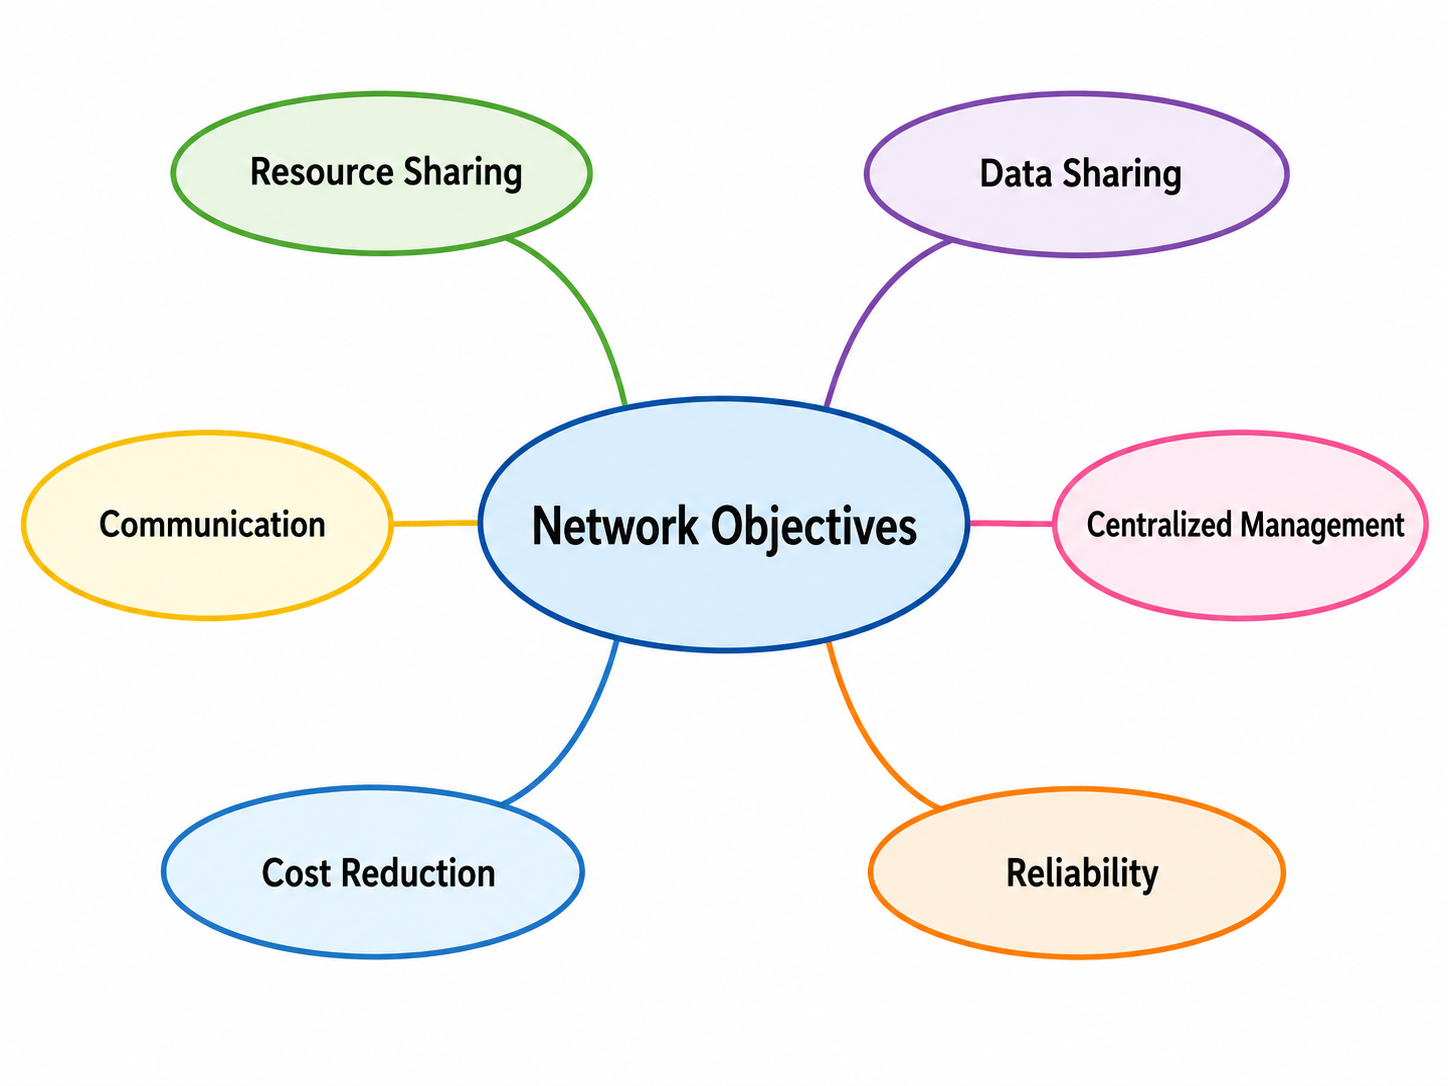
\includegraphics[width=0.92\textwidth]{chapters/Chapter02/images/network_objectives_mindmap.png}
}{
\fbox{
\parbox{0.90\textwidth}{
\centering
\vspace{0.7cm}
Network Objectives\\[8pt]
Resource Sharing \quad Data Sharing \quad Communication\\[6pt]
Centralized Management \quad Cost Reduction \quad Reliability
\vspace{0.7cm}
}}
}
\caption{কম্পিউটার নেটওয়ার্কের উদ্দেশ্য}
\end{figure}

\subsection{Resource Sharing}

\begin{definitionbox}{Resource Sharing}
একটি network-এর একাধিক user বা device একই hardware, software, data বা service ব্যবহার করতে পারাকে resource sharing বলা হয়।
\end{definitionbox}

Resource sharing computer network-এর সবচেয়ে গুরুত্বপূর্ণ উদ্দেশ্যগুলোর একটি। একটি printer network-এ share করলে lab-এর সব computer সেই printer ব্যবহার করতে পারে। একইভাবে file server, database server, internet connection, software license, storage device ইত্যাদিও share করা যায়।

\begin{keypointbox}{Resource sharing-এর উদাহরণ}
\begin{itemize}
\item এক printer অনেক computer ব্যবহার করা।
\item file server থেকে class note download করা।
\item office database একাধিক employee ব্যবহার করা।
\item এক internet connection router দিয়ে অনেক device-এ share করা।
\item cloud storage ব্যবহার করে file access করা।
\end{itemize}
\end{keypointbox}

\subsection{Data Sharing}

\begin{definitionbox}{Data Sharing}
Network-এর মাধ্যমে এক device থেকে অন্য device-এ file, document, image, audio, video বা database information আদান-প্রদান করাকে data sharing বলা হয়।
\end{definitionbox}

Data sharing-এর ফলে একই data অনেক user ব্যবহার করতে পারে। এতে duplicate file কমে, কাজ দ্রুত হয় এবং team collaboration সহজ হয়। তবে data sharing-এর ক্ষেত্রে permission, authentication ও backup গুরুত্বপূর্ণ।

\begin{examplebox}{বাস্তব উদাহরণ}
একটি college office-এ admission database server-এ রাখা হলো। Principal, office assistant এবং accounts section নির্দিষ্ট permission অনুযায়ী database access করতে পারে। এটি data sharing-এর উদাহরণ।
\end{examplebox}

\subsection{Communication}

Computer network-এর মাধ্যমে userরা দ্রুত communication করতে পারে। Email, instant messaging, video conference, file transfer, online meeting, VoIP call—সবই network-based communication।

\begin{keypointbox}{Network communication-এর সুবিধা}
\begin{itemize}
\item দ্রুত message পাঠানো যায়।
\item দূরবর্তী user-এর সাথে real-time communication করা যায়।
\item video conference ও online class করা যায়।
\item file transfer ও collaborative work সহজ হয়।
\item organization-এর internal communication দ্রুত হয়।
\end{itemize}
\end{keypointbox}

\subsection{Centralized Management}

\begin{definitionbox}{Centralized Management}
Network-এর data, user account, security, printer, software update ও access permission একটি central server বা administrator-এর মাধ্যমে পরিচালনা করার ব্যবস্থাকে centralized management বলা হয়।
\end{definitionbox}

Centralized management বড় office, bank, university ও data center-এর জন্য খুব গুরুত্বপূর্ণ। এতে user account control, password policy, file permission, software update, backup এবং security monitoring সহজ হয়।

\begin{examplebox}{সহজ উদাহরণ}
School lab-এর সব computer-এ আলাদা আলাদা software install না করে server বা administrator centralভাবে software update করলে সময় ও খরচ কমে।
\end{examplebox}

\subsection{Cost Reduction}

Network ব্যবহার করলে hardware ও service share করা যায়। এতে প্রতিটি computer-এর জন্য আলাদা printer, storage বা internet connection প্রয়োজন হয় না। ফলে cost কমে।

\begin{keypointbox}{Cost reduction-এর কারণ}
\begin{itemize}
\item এক printer অনেক computer ব্যবহার করতে পারে।
\item এক internet connection অনেক device-এ share করা যায়।
\item central storage ব্যবহারে আলাদা storage cost কমে।
\item software ও maintenance centralভাবে manage করা যায়।
\item office automation-এর ফলে সময় ও শ্রম কম লাগে।
\end{itemize}
\end{keypointbox}

\subsection{Reliability ও Backup}

Network ব্যবহার করলে data server বা cloud storage-এ backup রাখা যায়। কোনো computer নষ্ট হলেও server বা backup থেকে data restore করা সম্ভব। বড় organization-এ data loss কমাতে network backup system গুরুত্বপূর্ণ।

\begin{mistakebox}{Common mistake}
অনেকে ভাবে network শুধু internet ব্যবহারের জন্য তৈরি করা হয়। আসলে network-এর উদ্দেশ্য resource sharing, data sharing, communication, security, backup, centralized management এবং cost reduction—সবই।
\end{mistakebox}

\subsection{কম্পিউটার নেটওয়ার্কের সুবিধা}

\begin{keypointbox}{সুবিধা}
\begin{itemize}
\item data ও resource সহজে share করা যায়।
\item communication দ্রুত হয়।
\item printer, storage, internet connection share করে cost কমানো যায়।
\item central management ও monitoring করা যায়।
\item data backup ও recovery সহজ হয়।
\item team work ও collaboration বৃদ্ধি পায়।
\item দূরবর্তী access ও cloud service ব্যবহার করা যায়।
\end{itemize}
\end{keypointbox}

\subsection{কম্পিউটার নেটওয়ার্কের অসুবিধা}

\begin{keypointbox}{অসুবিধা}
\begin{itemize}
\item network setup ও maintenance cost থাকতে পারে।
\item security risk থাকে; unauthorized access হতে পারে।
\item virus বা malware network-এর মাধ্যমে ছড়াতে পারে।
\item server down হলে অনেক user service পেতে সমস্যা হতে পারে।
\item skilled network administrator দরকার হতে পারে।
\item network congestion হলে speed কমে যেতে পারে।
\item data privacy রক্ষা করা challenging হতে পারে।
\end{itemize}
\end{keypointbox}

\subsection{কম্পিউটার নেটওয়ার্কের প্রকারভেদ}

Computer network বিভিন্ন ভিত্তিতে শ্রেণিবিভাগ করা যায়। HSC ICT-তে সবচেয়ে গুরুত্বপূর্ণ হলো geographical area বা বিস্তৃতির ভিত্তিতে network classification।

\begin{figure}[H]
\centering
\IfFileExists{chapters/Chapter02/images/network_types_by_area.png}{
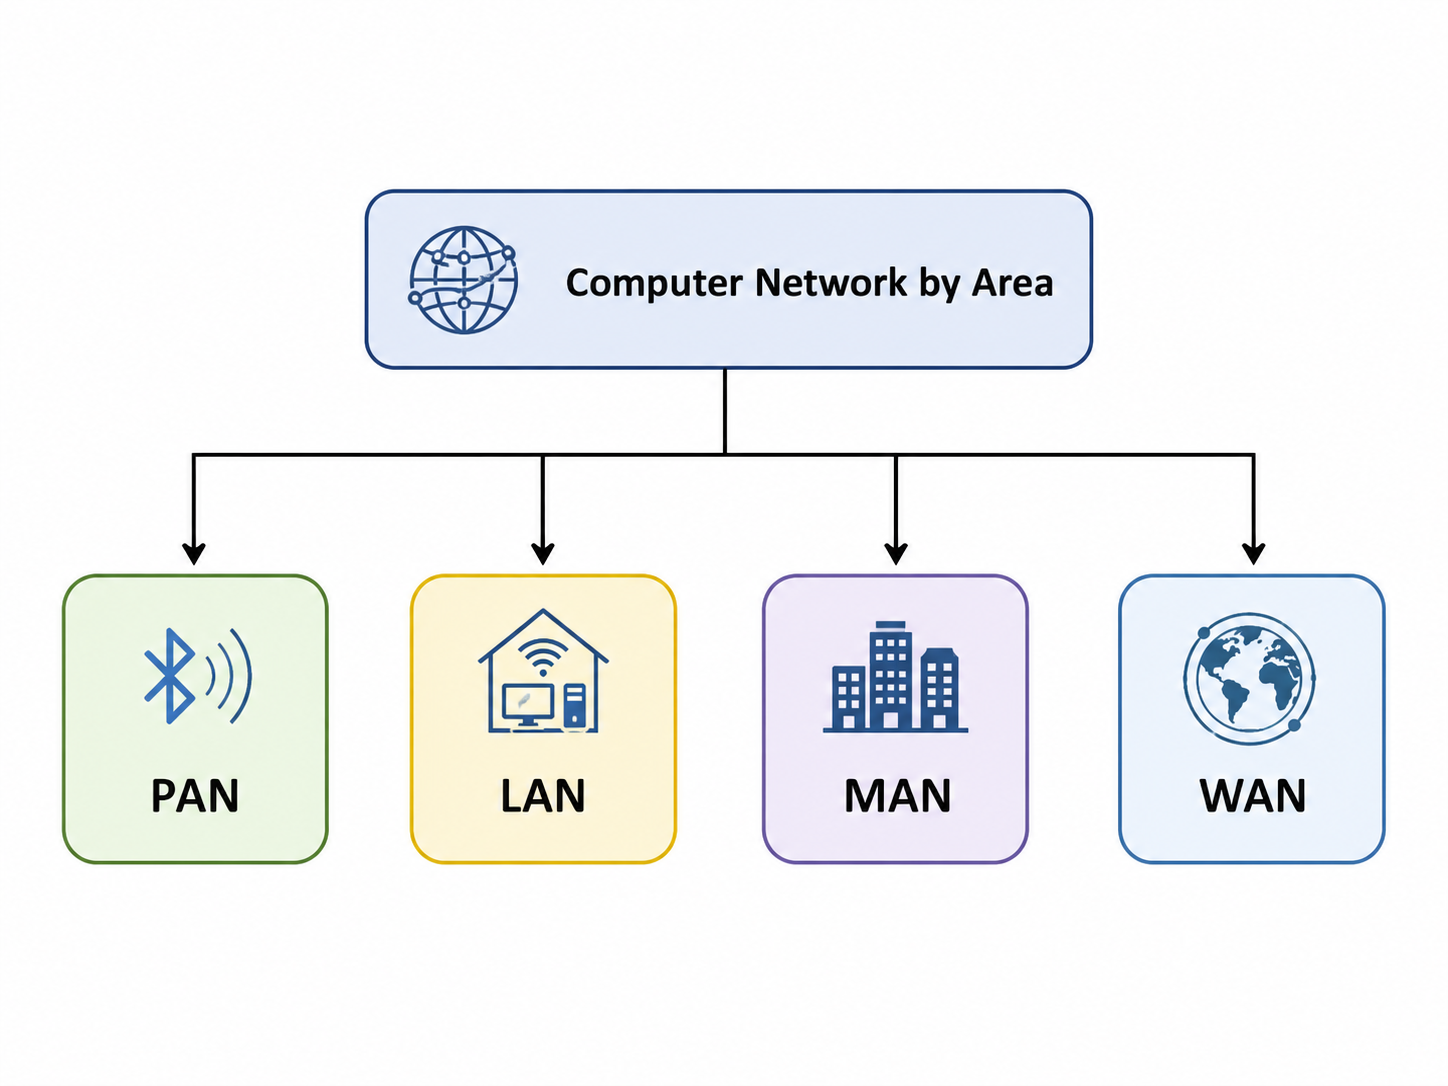
\includegraphics[width=0.92\textwidth]{chapters/Chapter02/images/network_types_by_area.png}
}{
\fbox{
\parbox{0.90\textwidth}{
\centering
\vspace{0.7cm}
Computer Network by Area\\[8pt]
PAN \quad LAN \quad MAN \quad WAN
\vspace{0.7cm}
}}
}
\caption{বিস্তৃতির ভিত্তিতে কম্পিউটার নেটওয়ার্কের প্রকারভেদ}
\end{figure}

\subsection{PAN: Personal Area Network}

\begin{definitionbox}{PAN}
একজন ব্যক্তির নিকটবর্তী personal device-গুলোর মধ্যে স্বল্প দূরত্বে data communication-এর জন্য গঠিত network-কে Personal Area Network বা PAN বলা হয়।
\end{definitionbox}

PAN সাধারণত একজন ব্যক্তির mobile, laptop, smartwatch, wireless earphone, keyboard, mouse, printer ইত্যাদি device-এর মধ্যে তৈরি হয়। Bluetooth, USB cable, infrared বা Wi-Fi Direct ব্যবহার করে PAN তৈরি হতে পারে। PAN-এর coverage সাধারণত খুব ছোট, যেমন কয়েক meter বা personal workspace-এর মধ্যে।

\begin{keypointbox}{PAN-এর বৈশিষ্ট্য}
\begin{itemize}
\item ব্যক্তিগত device-এর মধ্যে communication হয়।
\item coverage area খুব ছোট।
\item সাধারণত low power technology ব্যবহৃত হয়।
\item Bluetooth-based connection PAN-এর পরিচিত উদাহরণ।
\item mobile phone, smartwatch, earphone, keyboard, mouse connect করতে ব্যবহৃত হয়।
\end{itemize}
\end{keypointbox}

\begin{examplebox}{PAN উদাহরণ}
Mobile phone-এর সাথে Bluetooth earphone, smartwatch ও wireless keyboard connect করলে সেটি PAN-এর উদাহরণ।
\end{examplebox}

\subsection{LAN: Local Area Network}

\begin{definitionbox}{LAN}
একটি ছোট geographical area, যেমন room, lab, building, office বা campus-এর মধ্যে computer ও device-গুলোকে সংযুক্ত করে তৈরি network-কে Local Area Network বা LAN বলা হয়।
\end{definitionbox}

LAN সবচেয়ে বেশি ব্যবহৃত network type। School computer lab, office network, home Wi-Fi network, library network ইত্যাদি LAN-এর উদাহরণ। LAN সাধারণত high speed communication দেয় এবং organization নিজেই এটি manage করতে পারে।

\begin{keypointbox}{LAN-এর বৈশিষ্ট্য}
\begin{itemize}
\item ছোট area cover করে।
\item data transfer speed তুলনামূলক বেশি।
\item ownership সাধারণত private বা organization-based।
\item twisted pair cable, switch, router, Wi-Fi access point ব্যবহার হতে পারে।
\item resource sharing ও file sharing-এর জন্য উপযোগী।
\item maintenance তুলনামূলক সহজ।
\end{itemize}
\end{keypointbox}

\begin{examplebox}{LAN উদাহরণ}
College computer lab-এর সব computer switch-এর মাধ্যমে connected থাকলে সেটি LAN।
\end{examplebox}

\subsection{MAN: Metropolitan Area Network}

\begin{definitionbox}{MAN}
একটি city বা metropolitan area-এর মধ্যে একাধিক LAN বা network-কে সংযুক্ত করে তৈরি বৃহত্তর network-কে Metropolitan Area Network বা MAN বলা হয়।
\end{definitionbox}

MAN সাধারণত LAN-এর চেয়ে বড় কিন্তু WAN-এর চেয়ে ছোট। একটি শহরের বিভিন্ন branch office, bank branch, university campus বা cable TV network MAN-এর উদাহরণ হতে পারে।

\begin{keypointbox}{MAN-এর বৈশিষ্ট্য}
\begin{itemize}
\item একটি শহর বা metropolitan area cover করে।
\item একাধিক LAN সংযুক্ত করতে পারে।
\item LAN-এর চেয়ে coverage বেশি।
\item WAN-এর তুলনায় area ছোট।
\item city-wide broadband, cable TV network বা organization branch connection-এ ব্যবহৃত হতে পারে।
\end{itemize}
\end{keypointbox}

\subsection{WAN: Wide Area Network}

\begin{definitionbox}{WAN}
দেশ, মহাদেশ বা বিশ্বব্যাপী বিস্তৃত বড় geographical area জুড়ে computer ও network-গুলোকে সংযুক্ত করে তৈরি network-কে Wide Area Network বা WAN বলা হয়।
\end{definitionbox}

WAN হলো সবচেয়ে বড় network type। Internet হলো WAN-এর সবচেয়ে পরিচিত উদাহরণ। WAN ব্যবহার করে বিভিন্ন শহর, দেশ বা continent-এর network connected থাকে। WAN-এ leased line, optical fiber backbone, satellite link, microwave link, submarine cable ইত্যাদি ব্যবহার হতে পারে।

\begin{keypointbox}{WAN-এর বৈশিষ্ট্য}
\begin{itemize}
\item খুব বড় geographical area cover করে।
\item দেশ-বিদেশের network সংযুক্ত করে।
\item LAN ও MAN-এর তুলনায় বেশি complex।
\item public/private telecommunication infrastructure ব্যবহার করতে পারে।
\item internet WAN-এর সবচেয়ে পরিচিত উদাহরণ।
\item cost ও management complexity বেশি হতে পারে।
\end{itemize}
\end{keypointbox}

\begin{figure}[H]
\centering
\IfFileExists{chapters/Chapter02/images/pan_lan_man_wan_scale.png}{
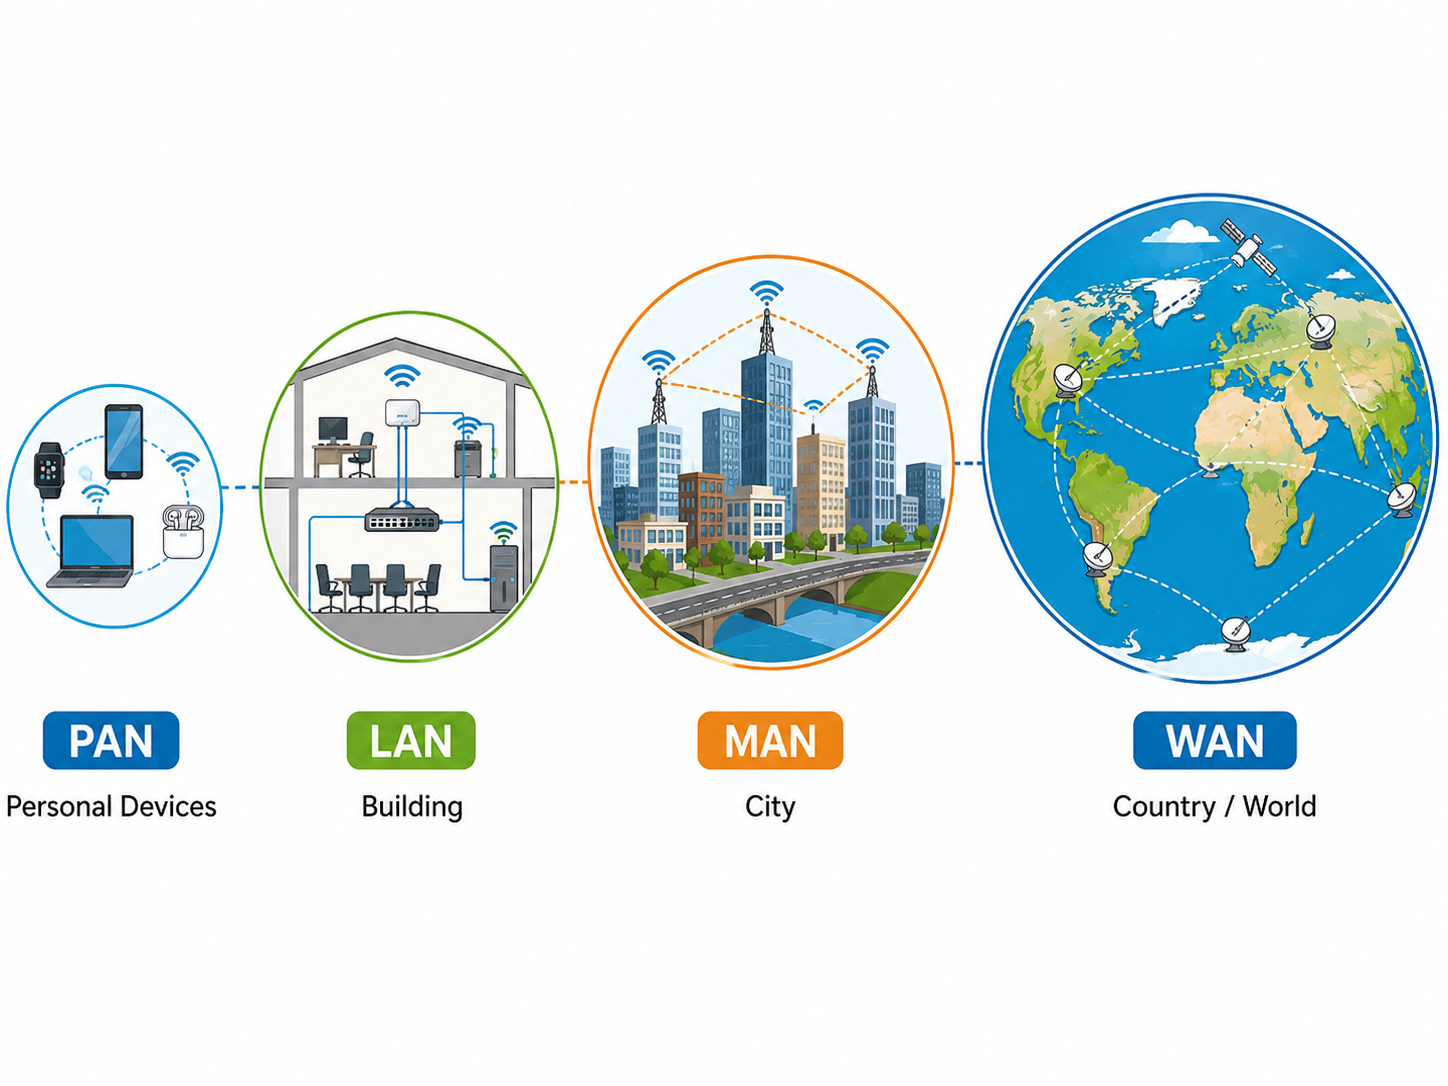
\includegraphics[width=0.92\textwidth]{chapters/Chapter02/images/pan_lan_man_wan_scale.png}
}{
\fbox{
\parbox{0.90\textwidth}{
\centering
\vspace{0.7cm}
PAN: Personal Devices\\[4pt]
LAN: Room / Building\\[4pt]
MAN: City\\[4pt]
WAN: Country / World
\vspace{0.7cm}
}}
}
\caption{PAN, LAN, MAN ও WAN-এর coverage scale}
\end{figure}

\subsection{PAN, LAN, MAN ও WAN-এর পার্থক্য}

\begin{center}
\begin{tabular}{|p{0.14\textwidth}|p{0.20\textwidth}|p{0.26\textwidth}|p{0.28\textwidth}|}
\hline
\textbf{Network} & \textbf{Coverage} & \textbf{ব্যবহার} & \textbf{উদাহরণ} \\
\hline
PAN & ব্যক্তিগত ছোট area & personal device connection & Mobile, smartwatch, Bluetooth earphone \\
\hline
LAN & room, lab, building, campus & local resource sharing & School lab, office network, home Wi-Fi \\
\hline
MAN & city/metropolitan area & city-wide network connection & City broadband, bank branches in a city \\
\hline
WAN & country/worldwide & long-distance communication & Internet, international bank network \\
\hline
\end{tabular}
\end{center}

\begin{boardbox}{বোর্ড ফোকাস}
PAN, LAN, MAN, WAN-এর প্রশ্নে শুধু পূর্ণরূপ লিখলে marks কমতে পারে। Coverage area, ব্যবহার ও উদাহরণ লিখতে হবে।
\end{boardbox}

\subsection{Network Architecture-এর ভিত্তিতে প্রকারভেদ}

Network কে control ও service ব্যবস্থার ভিত্তিতেও ভাগ করা যায়। HSC পর্যায়ে দুটি concept জানা গুরুত্বপূর্ণ:

\begin{itemize}
\item Peer-to-peer Network
\item Client-server Network
\end{itemize}

\subsection{Peer-to-peer Network}

\begin{definitionbox}{Peer-to-peer Network}
যে network-এ প্রতিটি computer প্রায় সমানভাবে resource share করে এবং আলাদা dedicated server থাকে না, তাকে peer-to-peer network বলা হয়।
\end{definitionbox}

Peer-to-peer network ছোট network-এর জন্য উপযোগী। এতে setup সহজ এবং cost কম। তবে security, backup ও centralized control দুর্বল হতে পারে।

\begin{keypointbox}{Peer-to-peer network-এর বৈশিষ্ট্য}
\begin{itemize}
\item dedicated server প্রয়োজন হয় না।
\item প্রতিটি computer resource share করতে পারে।
\item ছোট network-এর জন্য উপযোগী।
\item setup সহজ ও cost কম।
\item security ও management তুলনামূলক দুর্বল।
\end{itemize}
\end{keypointbox}

\subsection{Client-server Network}

\begin{definitionbox}{Client-server Network}
যে network-এ এক বা একাধিক server client computer-গুলোকে file, database, printer, website, authentication বা অন্য service প্রদান করে, তাকে client-server network বলা হয়।
\end{definitionbox}

Client-server network বড় organization, school, bank, hospital, office ও data center-এর জন্য উপযোগী। এখানে server centralভাবে data ও service manage করে। Security, backup, user permission এবং monitoring সহজ হয়।

\begin{keypointbox}{Client-server network-এর বৈশিষ্ট্য}
\begin{itemize}
\item dedicated server থাকে।
\item client server থেকে service নেয়।
\item centralized management করা যায়।
\item security ও backup ভালোভাবে control করা যায়।
\item বড় network-এর জন্য উপযোগী।
\item setup ও maintenance cost বেশি হতে পারে।
\end{itemize}
\end{keypointbox}

\begin{figure}[H]
\centering
\IfFileExists{chapters/Chapter02/images/client_server_vs_peer_to_peer.png}{
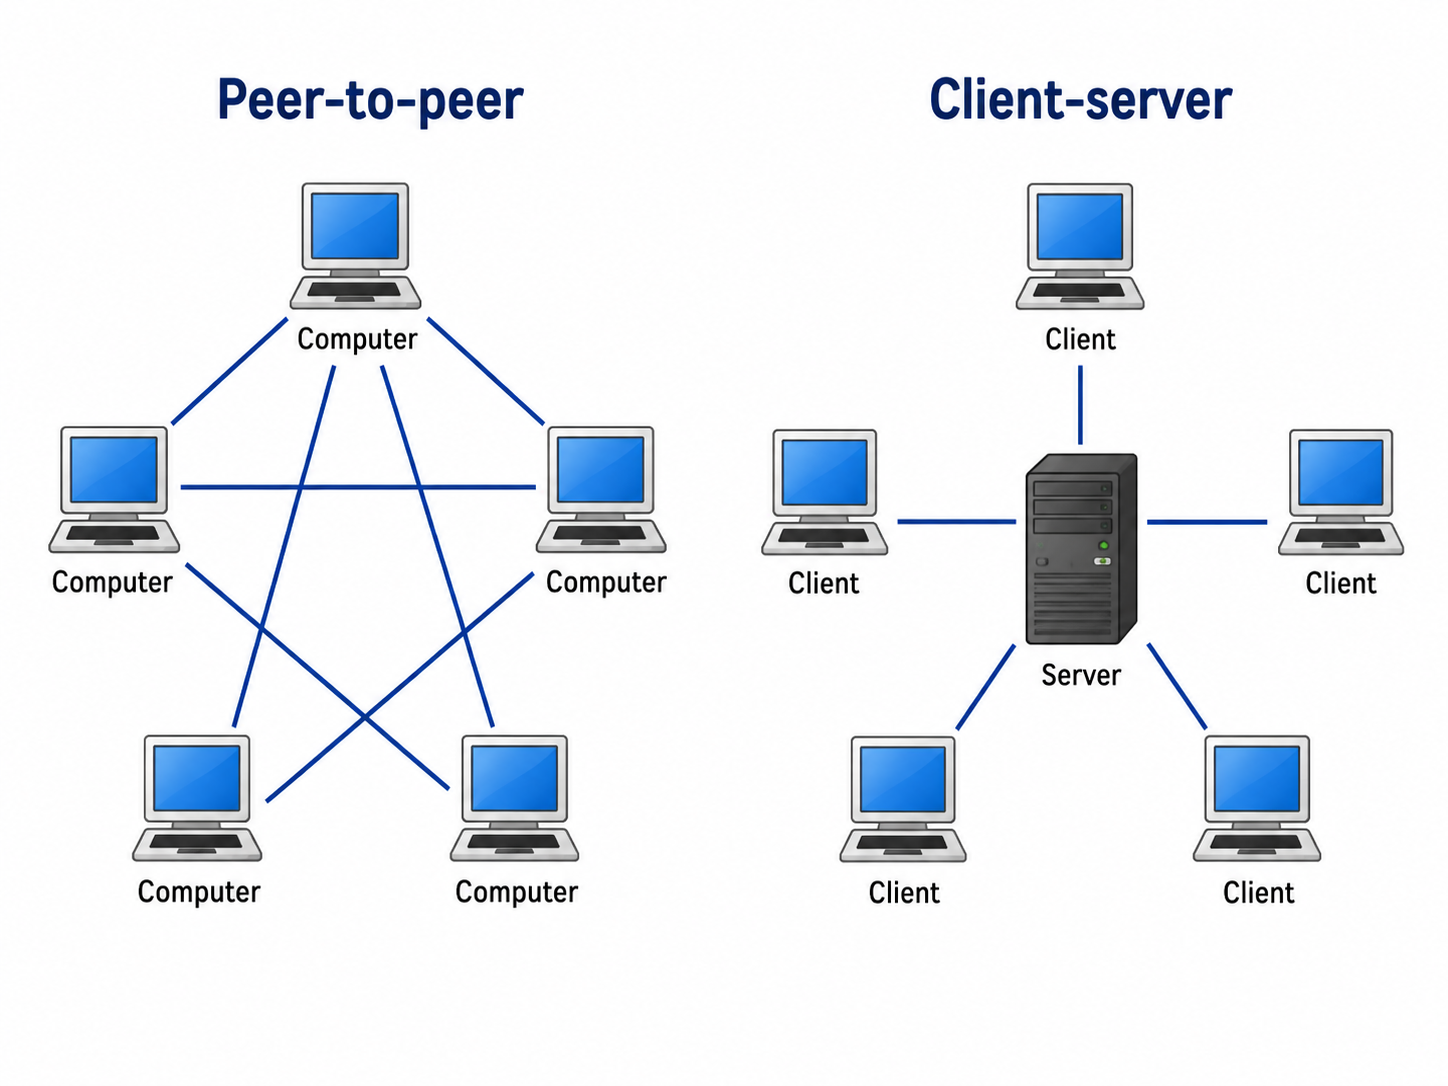
\includegraphics[width=0.92\textwidth]{chapters/Chapter02/images/client_server_vs_peer_to_peer.png}
}{
\fbox{
\parbox{0.90\textwidth}{
\centering
\vspace{0.7cm}
Peer-to-peer: Computer $\longleftrightarrow$ Computer $\longleftrightarrow$ Computer\\[8pt]
Client-server: Client Computers $\longleftrightarrow$ Server
\vspace{0.7cm}
}}
}
\caption{Client-server ও peer-to-peer network}
\end{figure}

\subsection{Client-server ও Peer-to-peer Network-এর পার্থক্য}

\begin{center}
\begin{tabular}{|p{0.24\textwidth}|p{0.30\textwidth}|p{0.30\textwidth}|}
\hline
\textbf{বিষয়} & \textbf{Peer-to-peer} & \textbf{Client-server} \\
\hline
Server & dedicated server নেই & dedicated server থাকে \\
\hline
Control & distributed & centralized \\
\hline
Cost & কম & বেশি \\
\hline
Security & তুলনামূলক কম & ভালোভাবে control করা যায় \\
\hline
উপযোগিতা & ছোট network & বড় organization network \\
\hline
Backup & কঠিন হতে পারে & central backup সহজ \\
\hline
Management & সহজ কিন্তু limited & professional management দরকার \\
\hline
\end{tabular}
\end{center}

\subsection{Internet, Intranet ও Extranet}

\begin{definitionbox}{Internet}
বিশ্বব্যাপী অসংখ্য network-এর সংযোগে গঠিত বৃহত্তম public network-কে Internet বলা হয়।
\end{definitionbox}

\begin{definitionbox}{Intranet}
কোনো organization-এর internal private network, যা সাধারণত organization-এর member বা employee-দের জন্য সীমাবদ্ধ থাকে, তাকে intranet বলা হয়।
\end{definitionbox}

\begin{definitionbox}{Extranet}
কোনো organization-এর private network-এর নির্দিষ্ট অংশ যখন authorized external user, partner, supplier বা customer-এর জন্য সীমিতভাবে উন্মুক্ত করা হয়, তাকে extranet বলা হয়।
\end{definitionbox}

\begin{figure}[H]
\centering
\IfFileExists{chapters/Chapter02/images/internet_intranet_extranet.png}{
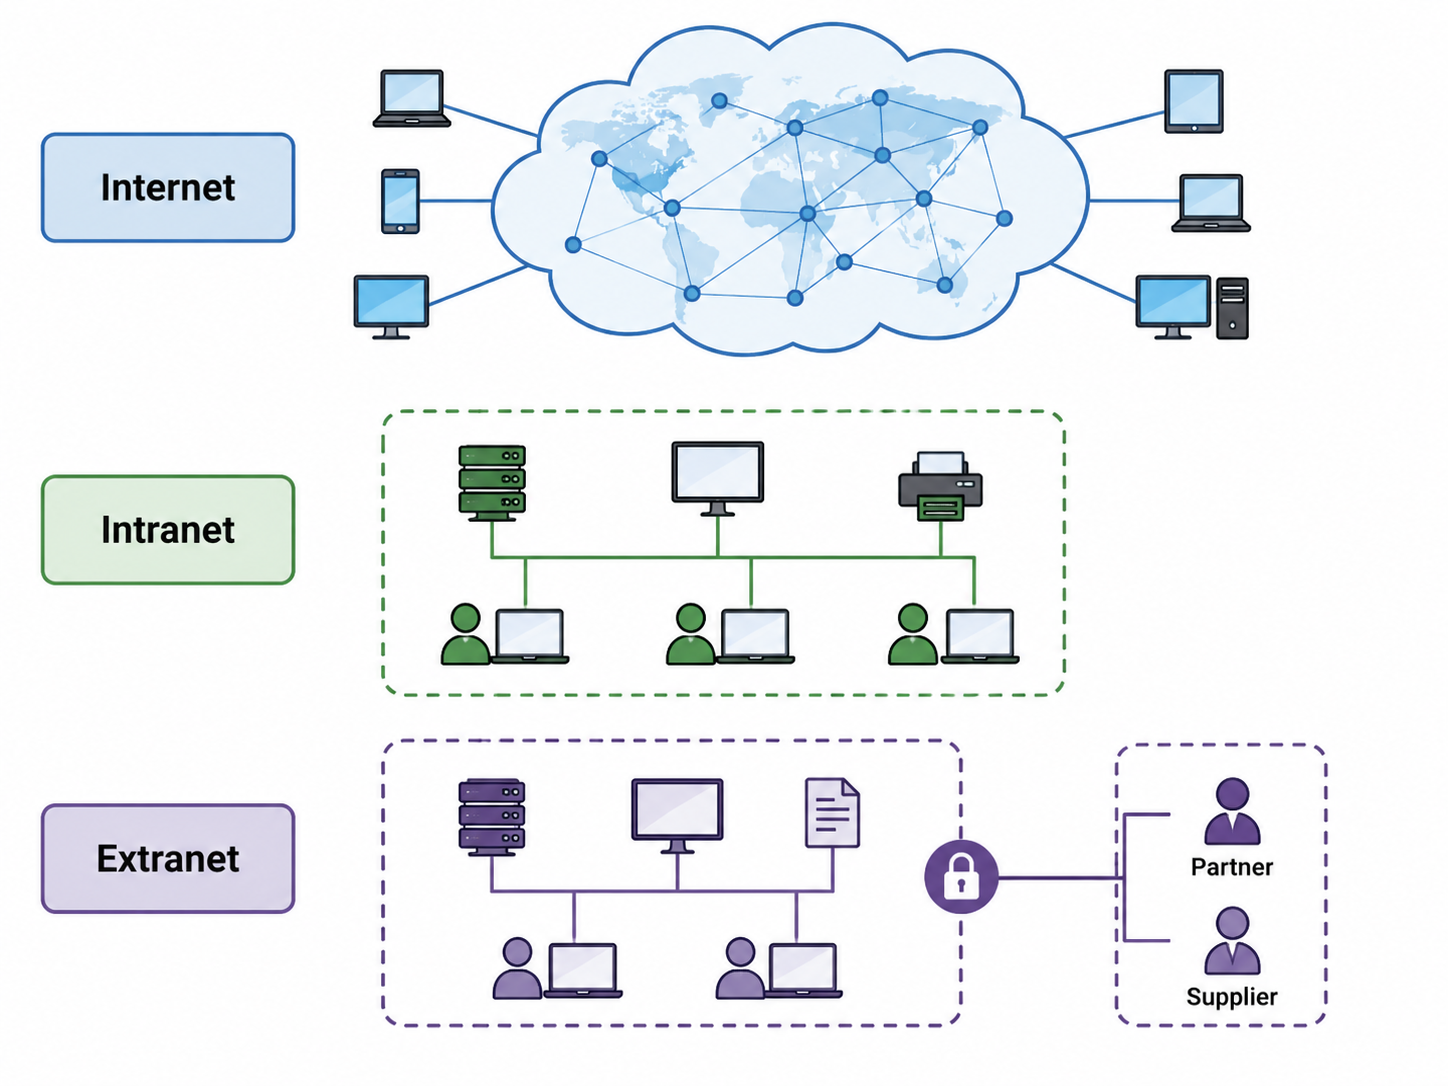
\includegraphics[width=0.92\textwidth]{chapters/Chapter02/images/internet_intranet_extranet.png}
}{
\fbox{
\parbox{0.90\textwidth}{
\centering
\vspace{0.7cm}
Internet: Public Global Network\\[6pt]
Intranet: Private Internal Network\\[6pt]
Extranet: Private Network with Authorized External Access
\vspace{0.7cm}
}}
}
\caption{Internet, Intranet ও Extranet}
\end{figure}

\begin{center}
\begin{tabular}{|p{0.20\textwidth}|p{0.32\textwidth}|p{0.32\textwidth}|}
\hline
\textbf{Network} & \textbf{Access} & \textbf{উদাহরণ} \\
\hline
Internet & public access & Website, email, online service \\
\hline
Intranet & organization internal access & Office internal portal \\
\hline
Extranet & authorized external access & Supplier/customer portal \\
\hline
\end{tabular}
\end{center}

\subsection{বাস্তব scenario অনুযায়ী network নির্বাচন}

\begin{center}
\begin{tabular}{|p{0.32\textwidth}|p{0.20\textwidth}|p{0.32\textwidth}|}
\hline
\textbf{পরিস্থিতি} & \textbf{Network type} & \textbf{কারণ} \\
\hline
Mobile phone ও Bluetooth earphone connection & PAN & personal device, short range \\
\hline
School computer lab & LAN & small area, resource sharing \\
\hline
এক শহরের বিভিন্ন bank branch connection & MAN & city-wide network \\
\hline
International company-এর country-to-country network & WAN & large geographical coverage \\
\hline
Office employee-only portal & Intranet & internal private access \\
\hline
Supplier login portal & Extranet & authorized external access \\
\hline
\end{tabular}
\end{center}

\subsection{Common Mistake Zone}

\begin{mistakebox}{Common mistake ১}
LAN মানে শুধু cable network নয়। Wi-Fi দিয়েও LAN তৈরি হতে পারে, যদি তা local area-এর মধ্যে network তৈরি করে।
\end{mistakebox}

\begin{mistakebox}{Common mistake ২}
Internet ও WAN একই কথা নয়। Internet হলো WAN-এর সবচেয়ে বড় ও পরিচিত উদাহরণ; কিন্তু সব WAN internet নয়।
\end{mistakebox}

\begin{mistakebox}{Common mistake ৩}
PAN ও LAN গুলিয়ে ফেলা যাবে না। PAN ব্যক্তিগত device-এর ছোট network, LAN হলো room/building/campus-এর local network।
\end{mistakebox}

\begin{mistakebox}{Common mistake ৪}
Peer-to-peer network-এ কোনো server concept থাকতে পারে না—এভাবে বলা ঠিক নয়। Dedicated central server থাকে না, কিন্তু প্রতিটি computer নিজ resource share করতে পারে।
\end{mistakebox}

\subsection{Exam-style প্রশ্ন ও উত্তর}

\begin{boardbox}{সংক্ষিপ্ত প্রশ্ন: Computer network কী?}
দুই বা ততোধিক computer, device বা node-কে communication medium ও protocol-এর মাধ্যমে যুক্ত করে data, information, hardware, software ও network resource আদান-প্রদানের ব্যবস্থাকে computer network বলা হয়। যেমন—school lab network, office network, internet।
\end{boardbox}

\begin{boardbox}{সংক্ষিপ্ত প্রশ্ন: Computer network-এর উদ্দেশ্য লেখ।}
Computer network-এর প্রধান উদ্দেশ্য হলো resource sharing, data sharing, দ্রুত communication, centralized management, cost reduction, backup ও reliability নিশ্চিত করা। Network-এর মাধ্যমে printer, file, database, internet connection ও software service share করা যায়।
\end{boardbox}

\begin{boardbox}{সংক্ষিপ্ত প্রশ্ন: LAN কী?}
একটি ছোট geographical area, যেমন room, lab, building, office বা campus-এর মধ্যে computer ও device-গুলোকে সংযুক্ত করে তৈরি network-কে LAN বা Local Area Network বলা হয়। School computer lab, office network ও home Wi-Fi LAN-এর উদাহরণ।
\end{boardbox}

\begin{boardbox}{পার্থক্য: LAN ও WAN}
LAN ছোট geographical area যেমন room, building বা campus-এর মধ্যে ব্যবহৃত হয় এবং সাধারণত high speed local communication দেয়। WAN দেশ, মহাদেশ বা বিশ্বব্যাপী বিস্তৃত network, যা long-distance communication করে। School lab network LAN-এর উদাহরণ, আর Internet WAN-এর উদাহরণ।
\end{boardbox}

\begin{boardbox}{পার্থক্য: Client-server ও Peer-to-peer Network}
Peer-to-peer network-এ dedicated server থাকে না এবং প্রতিটি computer resource share করতে পারে। এটি ছোট network-এর জন্য উপযোগী। Client-server network-এ dedicated server থাকে, client-রা server থেকে service নেয় এবং centralized management করা যায়। এটি বড় organization network-এর জন্য উপযোগী।
\end{boardbox}

\subsection{Brainstorming Critical Question}

\begin{practicebox}
একটি কলেজে নতুন digital system চালু করা হলো। Computer lab-এর ৪০টি computer একই printer ও internet connection ব্যবহার করছে। Principal office ও accounts section একই student database access করছে। College-এর দুইটি branch একই শহরে connected এবং head office অন্য জেলায় অবস্থিত।

\begin{enumerate}
\item ক. Computer network কী?
\item খ. Resource sharing কেন গুরুত্বপূর্ণ?
\item গ. Computer lab-এর network কোন type-এর হতে পারে? ব্যাখ্যা কর।
\item ঘ. একই শহরের branch connection ও অন্য জেলার head office connection-এর ক্ষেত্রে MAN ও WAN-এর ব্যবহার বিশ্লেষণ কর।
\end{enumerate}
\end{practicebox}

\subsection{১ মিনিটে রিভিশন}

\begin{recapbox}
\begin{itemize}
\item Computer network হলো connected device-এর system।
\item Networking হলো network তৈরি ও পরিচালনার process।
\item Network-এর উদ্দেশ্য: resource sharing, data sharing, communication, centralized management, cost reduction।
\item PAN ব্যক্তিগত device-এর ছোট network।
\item LAN room/building/campus-এর local network।
\item MAN city-wide network।
\item WAN country/worldwide network।
\item Internet হলো বিশ্বব্যাপী public network।
\item Intranet হলো organization-এর private internal network।
\item Extranet হলো limited external access সহ private network।
\item Peer-to-peer network ছোট network-এর জন্য সহজ ও কম খরচের।
\item Client-server network বড় organization-এর জন্য secure ও centrally managed।
\end{itemize}
\end{recapbox}

\subsection{অনুশীলন}

\begin{practicebox}
\textbf{MCQ}
\begin{enumerate}
\item দুই বা ততোধিক computer যুক্ত করে data ও resource sharing করার ব্যবস্থাকে কী বলে?\\
ক. Processor \quad খ. Computer network \quad গ. Monitor \quad ঘ. Keyboard

\item PAN-এর পূর্ণরূপ কী?\\
ক. Public Area Network \quad খ. Personal Area Network \quad গ. Private Access Node \quad ঘ. Protocol Area Number

\item School computer lab সাধারণত কোন network-এর উদাহরণ?\\
ক. PAN \quad খ. LAN \quad গ. MAN \quad ঘ. WAN

\item একটি শহরের বিভিন্ন branch office যুক্ত করলে কোন network হতে পারে?\\
ক. PAN \quad খ. LAN \quad গ. MAN \quad ঘ. Cache

\item Internet কোন network-এর সবচেয়ে পরিচিত উদাহরণ?\\
ক. WAN \quad খ. PAN \quad গ. ROM \quad ঘ. CPU

\item Client-server network-এ service প্রদান করে কোনটি?\\
ক. Client \quad খ. Server \quad গ. Mouse \quad ঘ. Keyboard

\item Office-এর internal private network কোনটি?\\
ক. Internet \quad খ. Intranet \quad গ. Extranet \quad ঘ. Bluetooth only

\item Bluetooth earphone ও mobile phone-এর network কোনটি?\\
ক. PAN \quad খ. WAN \quad গ. MAN \quad ঘ. PSTN
\end{enumerate}

\textbf{সংক্ষিপ্ত প্রশ্ন}
\begin{enumerate}
\item Computer network কী?
\item Networking বলতে কী বোঝায়?
\item Computer network-এর পাঁচটি উদ্দেশ্য লেখ।
\item Resource sharing কী? উদাহরণ দাও।
\item PAN, LAN, MAN ও WAN-এর মধ্যে পার্থক্য লেখ।
\item Client-server network কী?
\item Peer-to-peer network কী?
\item Internet, Intranet ও Extranet-এর পার্থক্য লেখ।
\item LAN ও WAN-এর মধ্যে পার্থক্য লেখ।
\item Network-এর সুবিধা ও অসুবিধা লেখ।
\end{enumerate}

\textbf{সৃজনশীল প্রশ্ন}
একটি hospital network তৈরি করা হচ্ছে। Doctor chamber-এর computer-গুলো একই printer ও patient database ব্যবহার করবে। Hospital-এর অন্য branch একই শহরে connected থাকবে। Head office অন্য দেশে অবস্থিত এবং online reporting system থাকবে। Supplier-রা নির্দিষ্ট portal দিয়ে medicine stock update করতে পারবে।

\begin{enumerate}
\item ক. LAN কী?
\item খ. Intranet private network কেন?
\item গ. Doctor chamber-এর computer network কোন type-এর? ব্যাখ্যা কর।
\item ঘ. branch, head office এবং supplier portal-এর ক্ষেত্রে MAN, WAN ও Extranet-এর ব্যবহার বিশ্লেষণ কর।
\end{enumerate}
\end{practicebox}
% Chapter 02.8: Network devices
\section{Network Devices}

\begin{itemize}
\item Hub
\item Switch
\item Router
\item Bridge
\item Gateway
\item Modem
\end{itemize}

\subsection{Device Functions}
\begin{itemize}
\item Packet forwarding
\item Addressing (MAC, IP)
\item Routing vs Switching
\end{itemize}

% Chapter 02.9: নেটওয়ার্ক টপোলজি
\section{নেটওয়ার্ক টপোলজি}

\begin{learningbox}
এই টপিক শেষে শিক্ষার্থী পারবে:
\begin{itemize}
\item নেটওয়ার্ক টপোলজি কী তা ব্যাখ্যা করতে।
\item Physical topology ও Logical topology-এর ধারণা বুঝতে।
\item Bus, Star, Ring, Mesh, Tree ও Hybrid topology ব্যাখ্যা করতে।
\item বিভিন্ন topology-এর সুবিধা, অসুবিধা ও ব্যবহার লিখতে।
\item বাস্তব network scenario থেকে উপযুক্ত topology নির্বাচন করতে।
\item বোর্ড পরীক্ষার জন্য comparison-based answer, short answer ও CQ answer লিখতে।
\end{itemize}
\end{learningbox}

\subsection{বাস্তব জীবনের শুরু}

একটি computer lab কল্পনা করো। সেখানে ৩০টি computer, ১টি server, ১টি printer এবং internet connection আছে। এখন প্রশ্ন হলো—এই device-গুলো কীভাবে পরস্পরের সাথে যুক্ত হবে?

সব computer কি একটি central switch-এর সাথে যুক্ত হবে? নাকি একটি single cable-এর সাথে সবাই connect থাকবে? নাকি প্রতিটি device অন্য প্রতিটি device-এর সাথে আলাদা link দিয়ে যুক্ত থাকবে?

Network-এর device বা node-গুলো কীভাবে সাজানো ও সংযুক্ত থাকবে—এই arrangement-ই হলো \textbf{network topology}।

\begin{keypointbox}{মূল ধারণা}
Network topology বুঝতে তিনটি প্রশ্ন মনে রাখো:
\begin{itemize}
\item network-এর device বা node-গুলো কীভাবে connected?
\item data কোন path দিয়ে flow করছে?
\item কোনো link বা central device নষ্ট হলে network কতটা প্রভাবিত হবে?
\end{itemize}
\end{keypointbox}

\subsection{নেটওয়ার্ক টপোলজি}

\begin{definitionbox}{নেটওয়ার্ক টপোলজি}
কম্পিউটার নেটওয়ার্কে computer, server, switch, router, printer ইত্যাদি node বা device কীভাবে পরস্পরের সাথে যুক্ত ও বিন্যস্ত থাকে, সেই physical বা logical arrangement-কে network topology বলা হয়।
\end{definitionbox}

সহজভাবে, topology হলো network-এর layout বা structure। এটি network design, cost, performance, reliability, troubleshooting এবং scalability-এর উপর সরাসরি প্রভাব ফেলে।

\begin{examplebox}{সহজ উদাহরণ}
\begin{itemize}
\item Computer lab-এ সব PC যদি একটি switch-এর সাথে connected থাকে, তাহলে সেটি Star topology-এর উদাহরণ।
\item পুরনো network-এ সব computer একটি backbone cable-এর সাথে যুক্ত থাকলে সেটি Bus topology।
\item প্রতিটি node যদি অন্য প্রতিটি node-এর সাথে link দ্বারা connected থাকে, সেটি Mesh topology।
\end{itemize}
\end{examplebox}

\begin{figure}[H]
\centering
\IfFileExists{chapters/Chapter02/images/network_topology_basic_concept.png}{
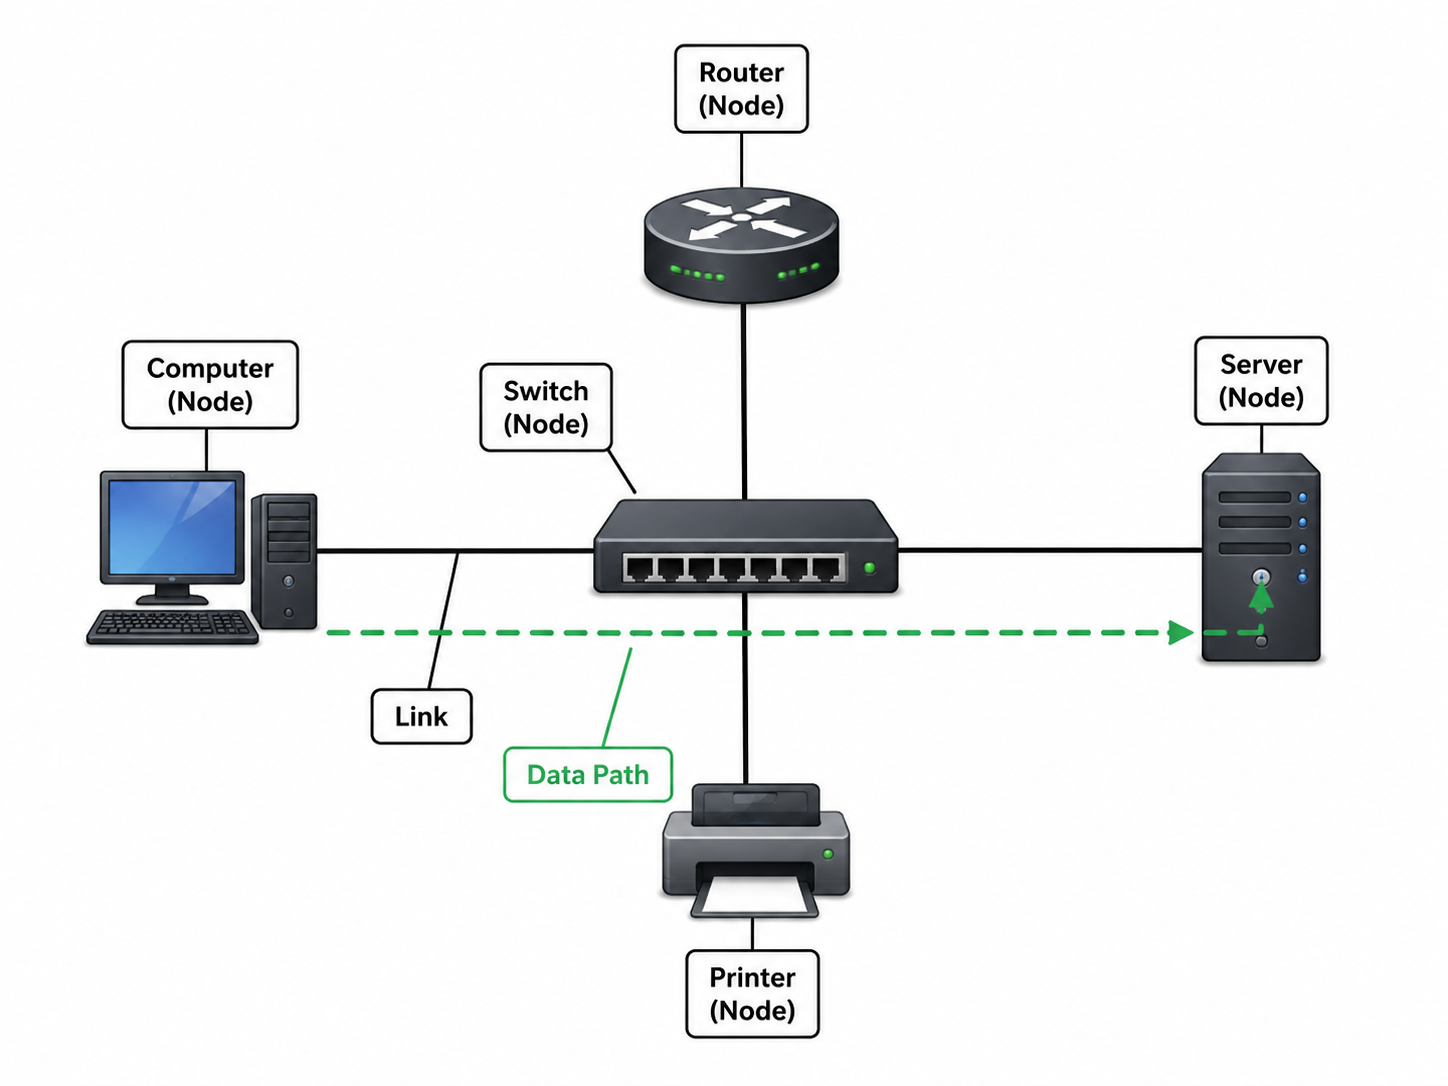
\includegraphics[width=0.92\textwidth]{chapters/Chapter02/images/network_topology_basic_concept.png}
}{
\fbox{
\parbox{0.90\textwidth}{
\centering
\vspace{0.7cm}
Network Topology[8pt]
Node + Link + Data Path[8pt]
Computer \quad Switch \quad Router \quad Server \quad Printer
\vspace{0.7cm}
}}
}
\caption{নেটওয়ার্ক টপোলজির মৌলিক ধারণা}
\end{figure}

\subsection{Network Topology কেন গুরুত্বপূর্ণ?}

একটি network কত দ্রুত কাজ করবে, কত সহজে manage করা যাবে, কোনো device নষ্ট হলে পুরো network বন্ধ হবে কি না, ভবিষ্যতে device add করা সহজ হবে কি না—এসব বিষয় topology-এর উপর নির্ভর করে।

\begin{keypointbox}{Topology গুরুত্বপূর্ণ কেন?}
\begin{itemize}
\item network design ও device placement বুঝতে সাহায্য করে।
\item network installation cost ও cable requirement নির্ধারণে সাহায্য করে।
\item data flow path বোঝা সহজ হয়।
\item fault finding বা troubleshooting সহজ হতে পারে।
\item network scalability বা ভবিষ্যতে expansion plan করা যায়।
\item failure হলে network কতটা প্রভাবিত হবে তা বিশ্লেষণ করা যায়।
\item performance ও traffic management-এর উপর প্রভাব ফেলে।
\end{itemize}
\end{keypointbox}

\subsection{Physical Topology ও Logical Topology}

Network topology দুইভাবে বোঝানো যায়:

\begin{itemize}
\item \textbf{Physical Topology}
\item \textbf{Logical Topology}
\end{itemize}

\begin{definitionbox}{Physical Topology}
Network-এর device, cable, switch, router ইত্যাদি hardware কীভাবে বাস্তবে বা physically connected থাকে, তাকে physical topology বলা হয়।
\end{definitionbox}

\begin{definitionbox}{Logical Topology}
Network-এ data কীভাবে বা কোন logical path দিয়ে flow করে, তাকে logical topology বলা হয়।
\end{definitionbox}

একই network-এর physical topology একরকম হলেও logical data flow ভিন্ন হতে পারে। তাই ভালো network design করতে physical connection এবং logical data flow—দুটিই বোঝা জরুরি।

\begin{center}
\begin{tabular}{|p{0.25\textwidth}|p{0.32\textwidth}|p{0.32\textwidth}|}
\hline
\textbf{বিষয়} & \textbf{Physical Topology} & \textbf{Logical Topology} \
\hline
মানে & device ও cable-এর বাস্তব arrangement & data flow-এর logical path \
\hline
Focus & hardware connection & data communication path \
\hline
দেখা যায় কি? & diagram বা বাস্তব cable layout দেখে বোঝা যায় & protocol ও data flow দেখে বোঝা যায় \
\hline
উদাহরণ & Star layout, Bus cable, Ring connection & data switch দিয়ে flow করা, token passing \
\hline
\end{tabular}
\end{center}

\begin{figure}[H]
\centering
\IfFileExists{chapters/Chapter02/images/physical_vs_logical_topology.png}{
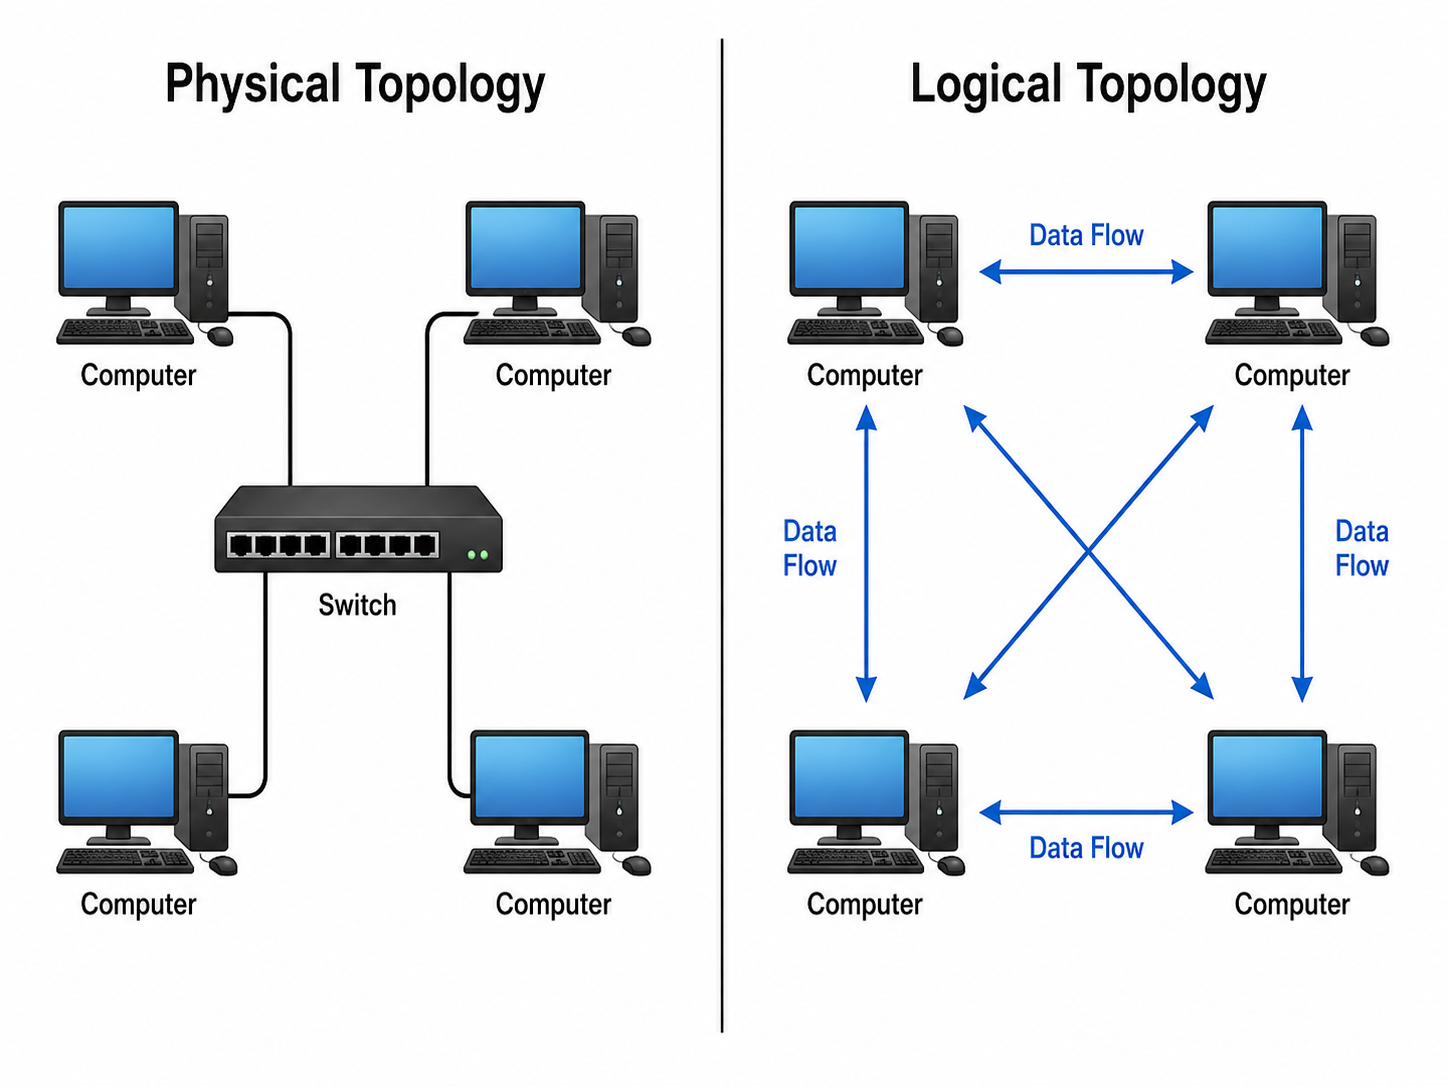
\includegraphics[width=0.92\textwidth]{chapters/Chapter02/images/physical_vs_logical_topology.png}
}{
\fbox{
\parbox{0.90\textwidth}{
\centering
\vspace{0.7cm}
Physical Topology: Actual device and cable layout[8pt]
Logical Topology: Data flow path
\vspace{0.7cm}
}}
}
\caption{Physical topology ও Logical topology}
\end{figure}

\subsection{নেটওয়ার্ক টপোলজির প্রকারভেদ}

HSC ICT-তে নিচের topology-গুলো সবচেয়ে গুরুত্বপূর্ণ:

\begin{itemize}
\item Bus Topology
\item Star Topology
\item Ring Topology
\item Mesh Topology
\item Tree Topology
\item Hybrid Topology
\end{itemize}

\begin{figure}[H]
\centering
\IfFileExists{chapters/Chapter02/images/network_topology_classification_tree.png}{
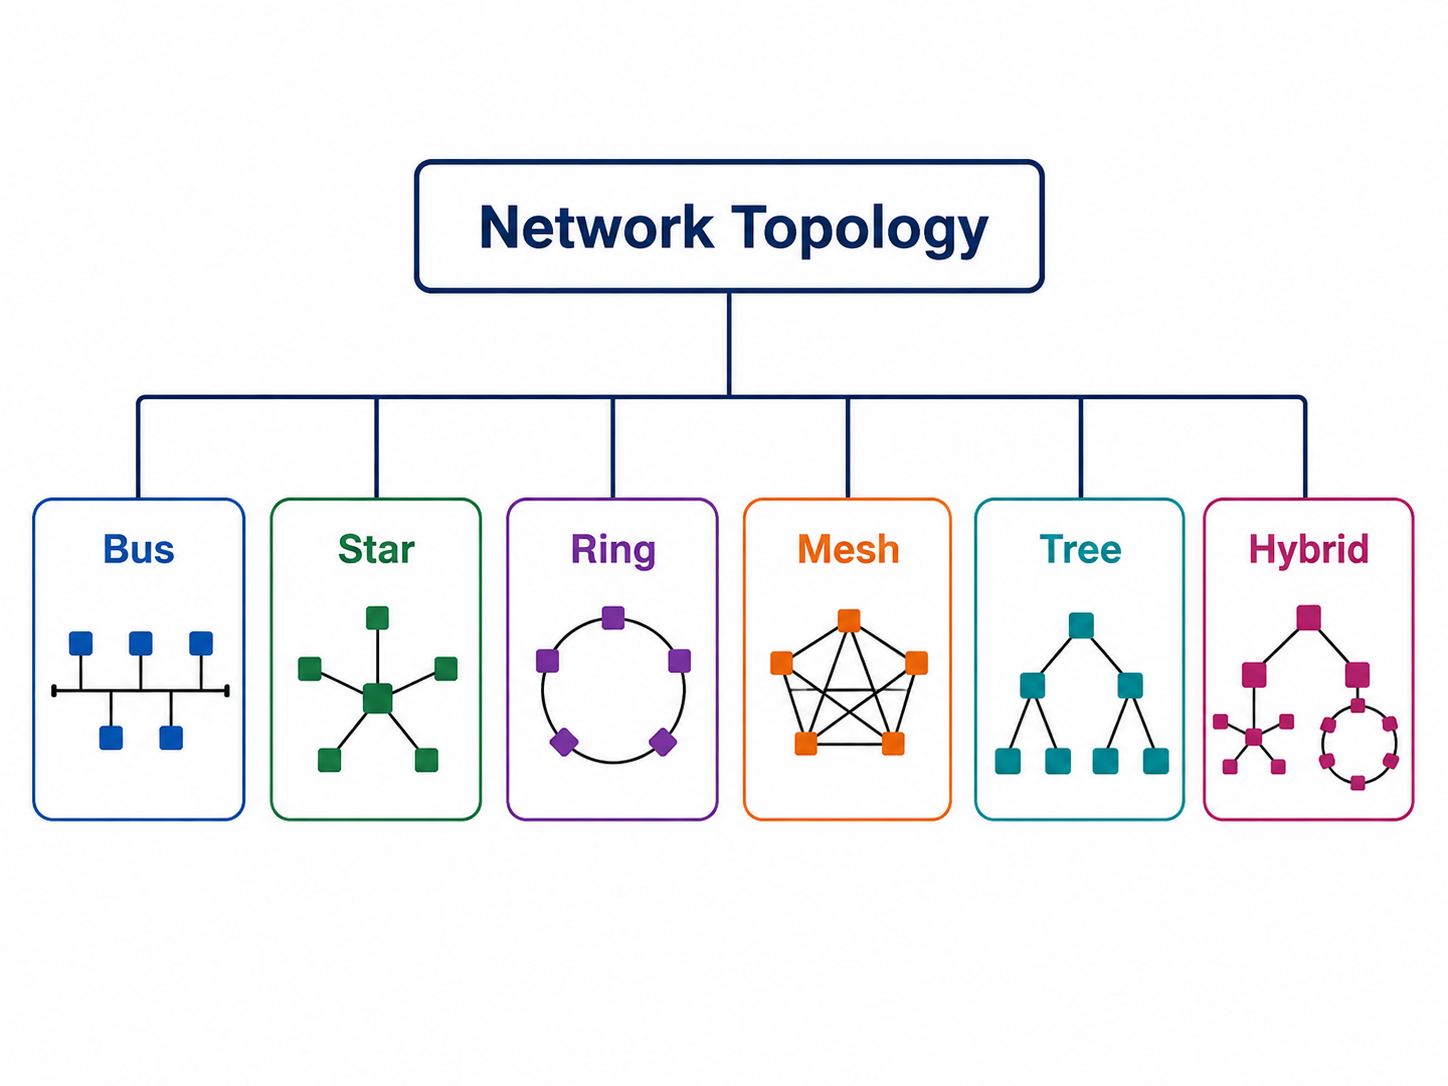
\includegraphics[width=0.92\textwidth]{chapters/Chapter02/images/network_topology_classification_tree.png}
}{
\fbox{
\parbox{0.90\textwidth}{
\centering
\vspace{0.7cm}
Network Topology[8pt]
Bus \quad Star \quad Ring \quad Mesh \quad Tree \quad Hybrid
\vspace{0.7cm}
}}
}
\caption{নেটওয়ার্ক টপোলজির প্রকারভেদ}
\end{figure}

\subsection{Bus Topology}

\begin{definitionbox}{Bus Topology}
যে network topology-তে সব node একটি common communication line বা backbone cable-এর সাথে যুক্ত থাকে, তাকে Bus topology বলা হয়।
\end{definitionbox}

Bus topology-তে একটি main cable বা backbone থাকে। সব computer বা node এই backbone cable-এর সাথে connected থাকে। কোনো node data পাঠালে data backbone cable দিয়ে travel করে এবং destination node সেটি গ্রহণ করে।

\begin{keypointbox}{Bus topology-এর বৈশিষ্ট্য}
\begin{itemize}
\item একটি main backbone cable থাকে।
\item সব node একই cable-এর সাথে connected থাকে।
\item installation তুলনামূলক সহজ।
\item cable কম লাগে, তাই cost কম হতে পারে।
\item backbone cable নষ্ট হলে পুরো network বন্ধ হতে পারে।
\item বেশি node যুক্ত হলে performance কমে যেতে পারে।
\item troubleshooting তুলনামূলক কঠিন হতে পারে।
\end{itemize}
\end{keypointbox}

\begin{figure}[H]
\centering
\IfFileExists{chapters/Chapter02/images/bus_topology_diagram.png}{
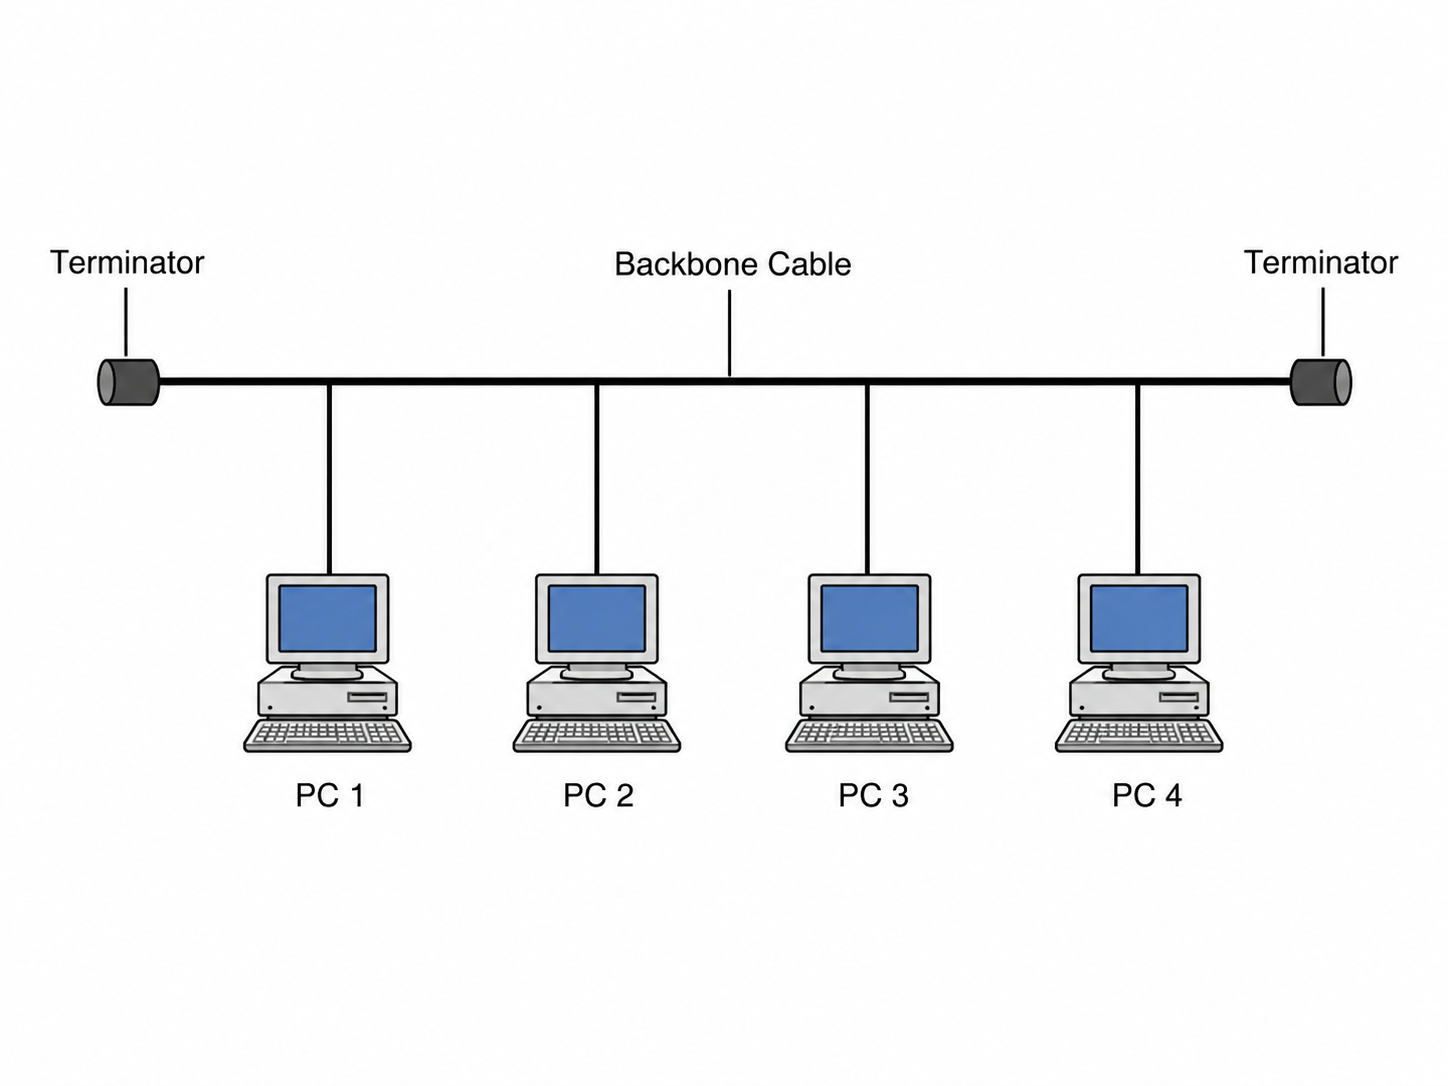
\includegraphics[width=0.92\textwidth]{chapters/Chapter02/images/bus_topology_diagram.png}
}{
\fbox{
\parbox{0.90\textwidth}{
\centering
\vspace{0.7cm}
PC 1 \quad PC 2 \quad PC 3 \quad PC 4[6pt]
\rule{0.75\textwidth}{1pt}[6pt]
Backbone Cable
\vspace{0.7cm}
}}
}
\caption{Bus topology}
\end{figure}

\begin{examplebox}{বাস্তব উদাহরণ}
পুরনো Ethernet network-এ coaxial cable ব্যবহার করে Bus topology দেখা যেত। ছোট বা temporary network design বোঝাতে এই topology ব্যবহার করা হয়।
\end{examplebox}

\begin{boardbox}{বোর্ড ফোকাস}
Bus topology-এর উত্তরে অবশ্যই “সব node একটি common backbone cable-এর সাথে যুক্ত থাকে” কথাটি লিখবে। Backbone cable failure হলে পুরো network প্রভাবিত হয়—এটি গুরুত্বপূর্ণ point।
\end{boardbox}

\subsection{Bus Topology-এর সুবিধা ও অসুবিধা}

\begin{center}
\begin{tabular}{|p{0.43\textwidth}|p{0.43\textwidth}|}
\hline
\textbf{সুবিধা} & \textbf{অসুবিধা} \
\hline
cable কম লাগে & backbone cable নষ্ট হলে network বন্ধ হতে পারে \
\hline
cost তুলনামূলক কম & বেশি node হলে traffic বাড়ে \
\hline
ছোট network-এ setup সহজ & fault খুঁজে বের করা কঠিন \
\hline
অস্থায়ী network-এর জন্য ব্যবহারযোগ্য & security ও performance তুলনামূলক কম \
\hline
\end{tabular}
\end{center}

\subsection{Star Topology}

\begin{definitionbox}{Star Topology}
যে network topology-তে সব node একটি central device যেমন switch বা hub-এর সাথে আলাদাভাবে connected থাকে, তাকে Star topology বলা হয়।
\end{definitionbox}

Star topology আধুনিক LAN-এ সবচেয়ে বেশি ব্যবহৃত topology-এর একটি। এখানে প্রতিটি computer আলাদা cable দ্বারা central switch বা hub-এর সাথে connected থাকে। কোনো একটি node-এর cable নষ্ট হলে সাধারণত শুধু সেই node affected হয়, পুরো network নয়। তবে central device নষ্ট হলে পুরো network প্রভাবিত হতে পারে।

\begin{keypointbox}{Star topology-এর বৈশিষ্ট্য}
\begin{itemize}
\item একটি central device থাকে।
\item প্রতিটি node central device-এর সাথে আলাদা link দিয়ে যুক্ত।
\item নতুন node add করা সহজ।
\item troubleshooting তুলনামূলক সহজ।
\item একটি node বা cable failure হলে পুরো network সাধারণত বন্ধ হয় না।
\item central device failure হলে network বন্ধ হতে পারে।
\item cable requirement bus topology-এর তুলনায় বেশি হতে পারে।
\end{itemize}
\end{keypointbox}

\begin{figure}[H]
\centering
\IfFileExists{chapters/Chapter02/images/star_topology_diagram.png}{
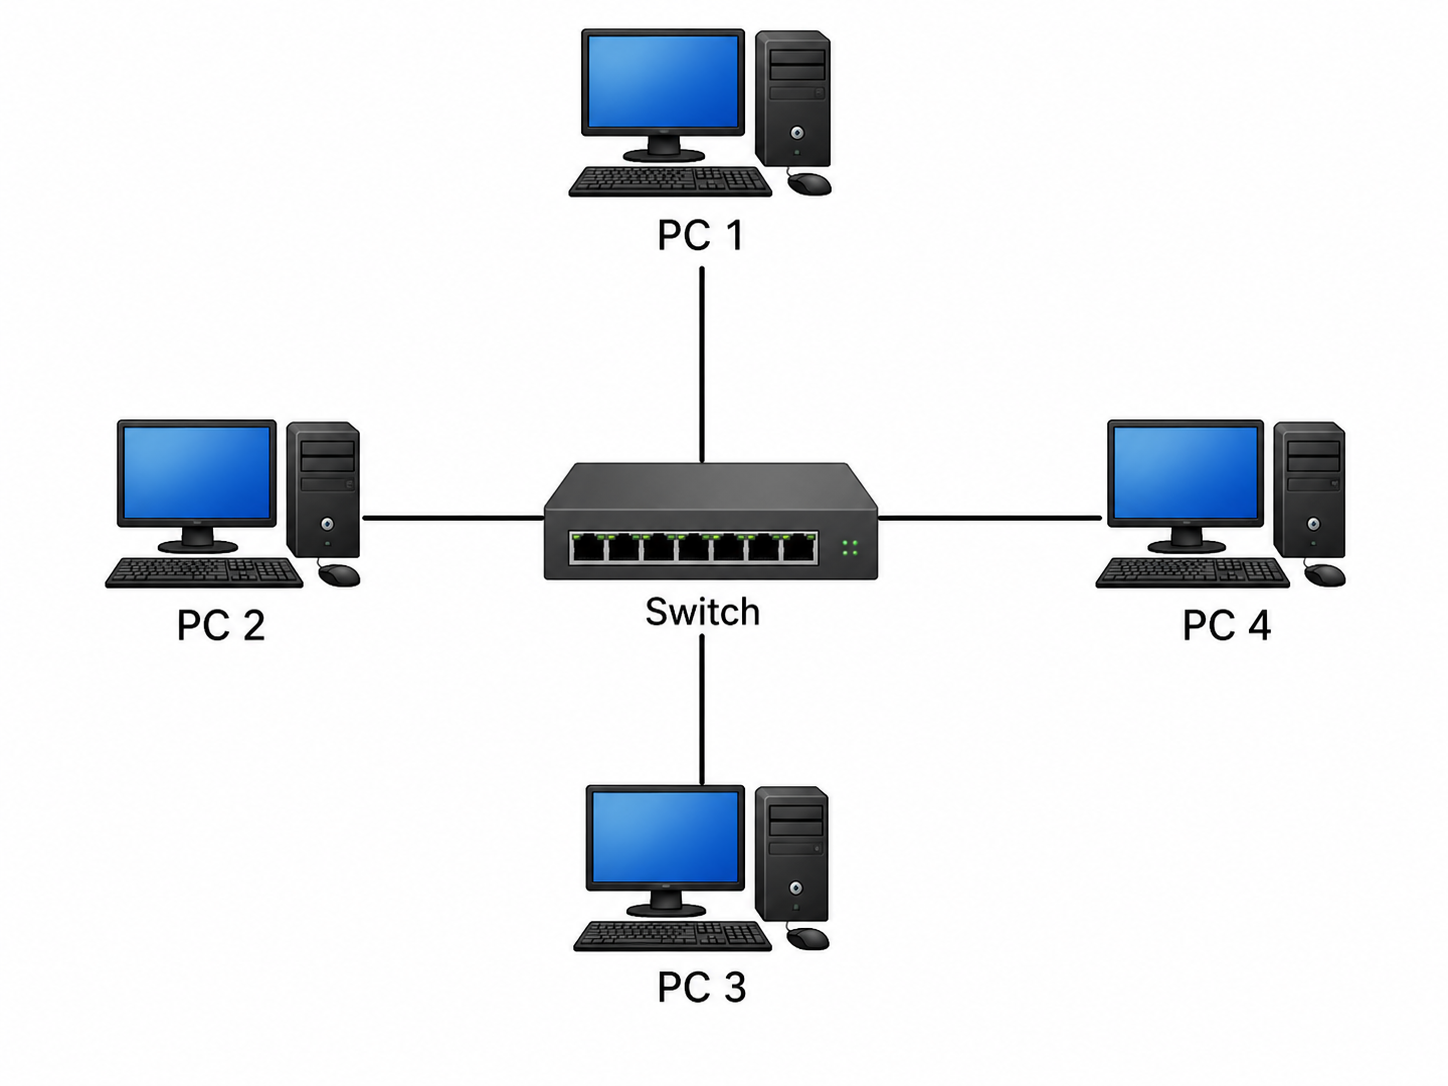
\includegraphics[width=0.86\textwidth]{chapters/Chapter02/images/star_topology_diagram.png}
}{
\fbox{
\parbox{0.84\textwidth}{
\centering
\vspace{0.7cm}
PC 1 \quad \quad PC 2[8pt]
\quad \diagdown \quad \quad \diagup[4pt]
\quad Switch / Hub[4pt]
\quad \diagup \quad \quad \diagdown[8pt]
PC 3 \quad \quad PC 4
\vspace{0.7cm}
}}
}
\caption{Star topology}
\end{figure}

\begin{examplebox}{বাস্তব উদাহরণ}
School computer lab বা office LAN-এ সাধারণত সব computer একটি switch-এর সাথে connected থাকে। এটি Star topology-এর বাস্তব উদাহরণ।
\end{examplebox}

\begin{boardbox}{বোর্ড ফোকাস}
Star topology-এর উত্তরে “central device” বা “switch/hub” উল্লেখ করা জরুরি। এটি আধুনিক LAN-এর জন্য খুব common topology।
\end{boardbox}

\subsection{Star Topology-এর সুবিধা ও অসুবিধা}

\begin{center}
\begin{tabular}{|p{0.43\textwidth}|p{0.43\textwidth}|}
\hline
\textbf{সুবিধা} & \textbf{অসুবিধা} \
\hline
installation ও management সহজ & central device নষ্ট হলে network বন্ধ হতে পারে \
\hline
নতুন node add করা সহজ & cable বেশি লাগে \
\hline
fault finding সহজ & central device-এর cost থাকে \
\hline
এক node failure পুরো network বন্ধ করে না & central device-এর উপর dependency বেশি \
\hline
performance ভালো হতে পারে, বিশেষ করে switch ব্যবহারে & বড় network-এ ভালো device দরকার \
\hline
\end{tabular}
\end{center}

\subsection{Ring Topology}

\begin{definitionbox}{Ring Topology}
যে network topology-তে প্রতিটি node তার পাশের দুইটি node-এর সাথে connected থাকে এবং সব node মিলে একটি closed loop বা ring তৈরি করে, তাকে Ring topology বলা হয়।
\end{definitionbox}

Ring topology-তে data সাধারণত একটি নির্দিষ্ট direction-এ node থেকে node-এ travel করে। একটি node data receive করে দেখে সেটি তার জন্য কি না। যদি তার জন্য না হয়, তাহলে পরবর্তী node-এ forward করে।

\begin{keypointbox}{Ring topology-এর বৈশিষ্ট্য}
\begin{itemize}
\item node-গুলো ring বা closed loop আকারে connected থাকে।
\item প্রতিটি node সাধারণত দুইটি neighboring node-এর সাথে যুক্ত থাকে।
\item data এক direction বা নির্দিষ্ট path ধরে travel করতে পারে।
\item collision কম হতে পারে।
\item কোনো node বা link failure হলে network প্রভাবিত হতে পারে।
\item troubleshooting তুলনামূলক জটিল হতে পারে।
\end{itemize}
\end{keypointbox}

\begin{figure}[H]
\centering
\IfFileExists{chapters/Chapter02/images/ring_topology_diagram.png}{
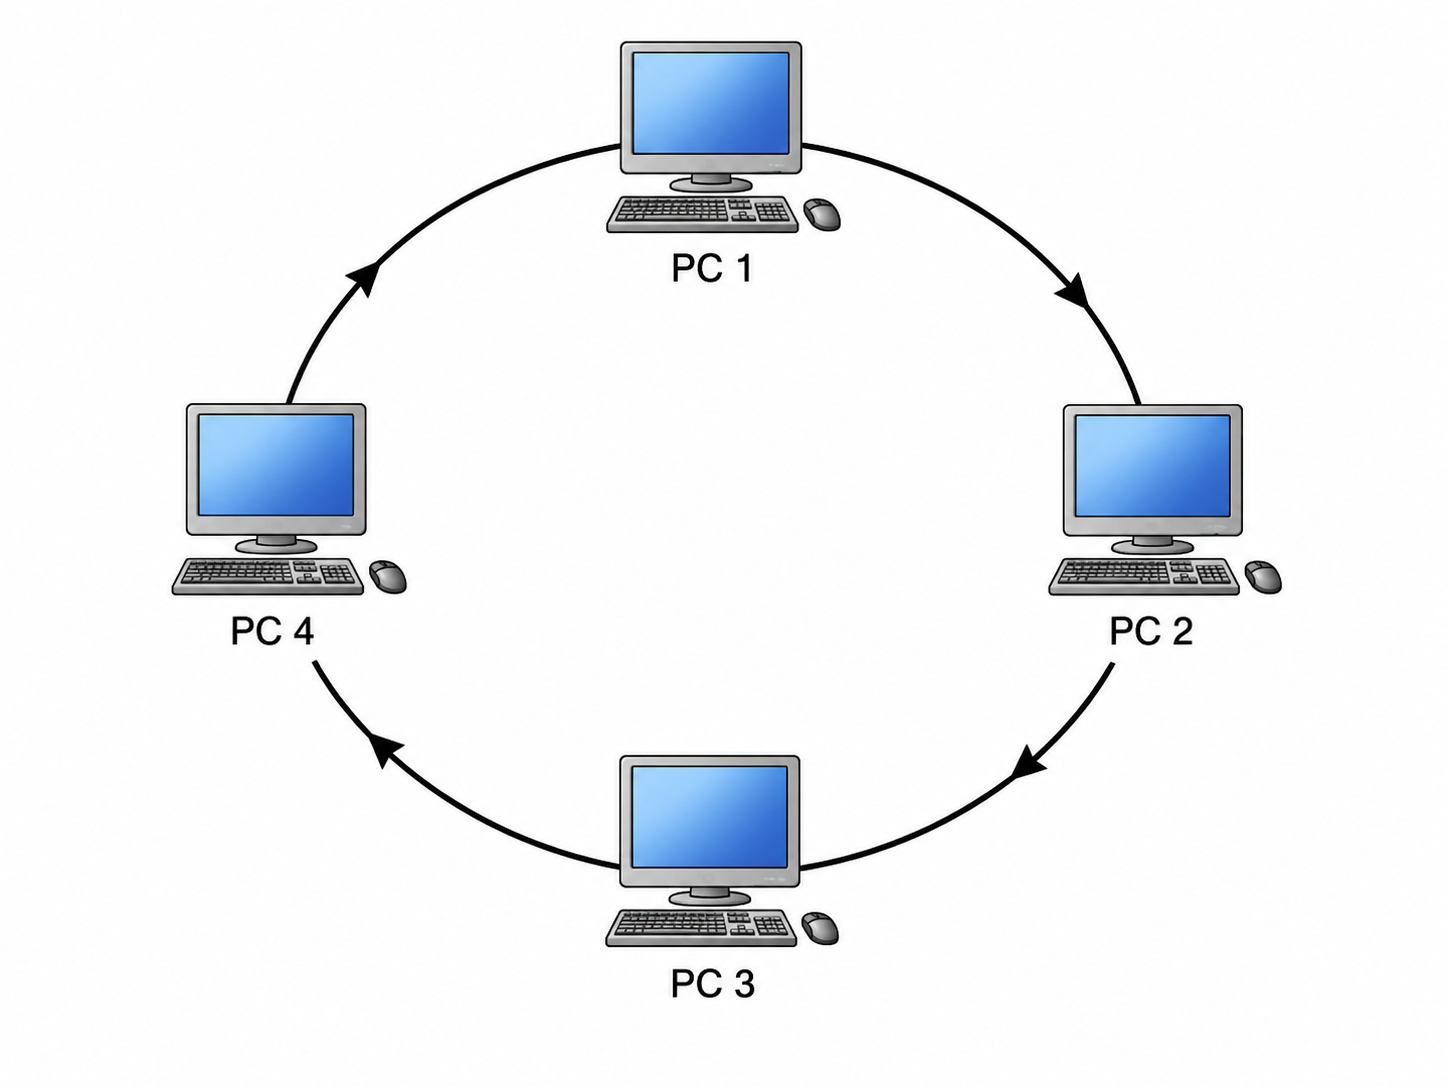
\includegraphics[width=0.86\textwidth]{chapters/Chapter02/images/ring_topology_diagram.png}
}{
\fbox{
\parbox{0.84\textwidth}{
\centering
\vspace{0.7cm}
PC 1 \quad $\longrightarrow$ \quad PC 2[8pt]
$\uparrow$ \qquad \qquad \qquad $\downarrow$[8pt]
PC 4 \quad $\longleftarrow$ \quad PC 3[8pt]
Closed Loop
\vspace{0.7cm}
}}
}
\caption{Ring topology}
\end{figure}

\begin{examplebox}{সহজ উদাহরণ}
যদি চারটি computer এমনভাবে connected থাকে যে PC1 থেকে PC2, PC2 থেকে PC3, PC3 থেকে PC4 এবং PC4 আবার PC1-এর সাথে connected, তাহলে এটি Ring topology।
\end{examplebox}

\subsection{Ring Topology-এর সুবিধা ও অসুবিধা}

\begin{center}
\begin{tabular}{|p{0.43\textwidth}|p{0.43\textwidth}|}
\hline
\textbf{সুবিধা} & \textbf{অসুবিধা} \
\hline
data নির্দিষ্ট path ধরে flow করে & একটি node/link failure network প্রভাবিত করতে পারে \
\hline
collision কম হতে পারে & troubleshooting কঠিন \
\hline
traffic predictable হতে পারে & নতুন node add করা তুলনামূলক কঠিন \
\hline
small controlled network-এ ব্যবহারযোগ্য & delay বাড়তে পারে কারণ data এক node থেকে অন্য node-এ যায় \
\hline
\end{tabular}
\end{center}

\subsection{Mesh Topology}

\begin{definitionbox}{Mesh Topology}
যে network topology-তে প্রতিটি node অন্য node-গুলোর সাথে সরাসরি বা একাধিক path দ্বারা connected থাকে, তাকে Mesh topology বলা হয়।
\end{definitionbox}

Mesh topology দুই ধরনের হতে পারে:

\begin{itemize}
\item \textbf{Full Mesh}: প্রতিটি node অন্য প্রতিটি node-এর সাথে সরাসরি connected।
\item \textbf{Partial Mesh}: সব node নয়, কিছু গুরুত্বপূর্ণ node একাধিক link দিয়ে connected।
\end{itemize}

Mesh topology অত্যন্ত reliable, কারণ একটি link নষ্ট হলেও alternative path দিয়ে data যেতে পারে। তবে বেশি cable, বেশি port এবং বেশি cost দরকার হয়।

\begin{keypointbox}{Mesh topology-এর বৈশিষ্ট্য}
\begin{itemize}
\item multiple path থাকে।
\item reliability বেশি।
\item fault tolerance ভালো।
\item security তুলনামূলক বেশি হতে পারে, কারণ dedicated link থাকতে পারে।
\item installation ও maintenance complex।
\item cable ও device port বেশি লাগে।
\item বড় backbone বা critical network-এ mesh concept গুরুত্বপূর্ণ।
\end{itemize}
\end{keypointbox}

\begin{figure}[H]
\centering
\IfFileExists{chapters/Chapter02/images/mesh_topology_diagram.png}{
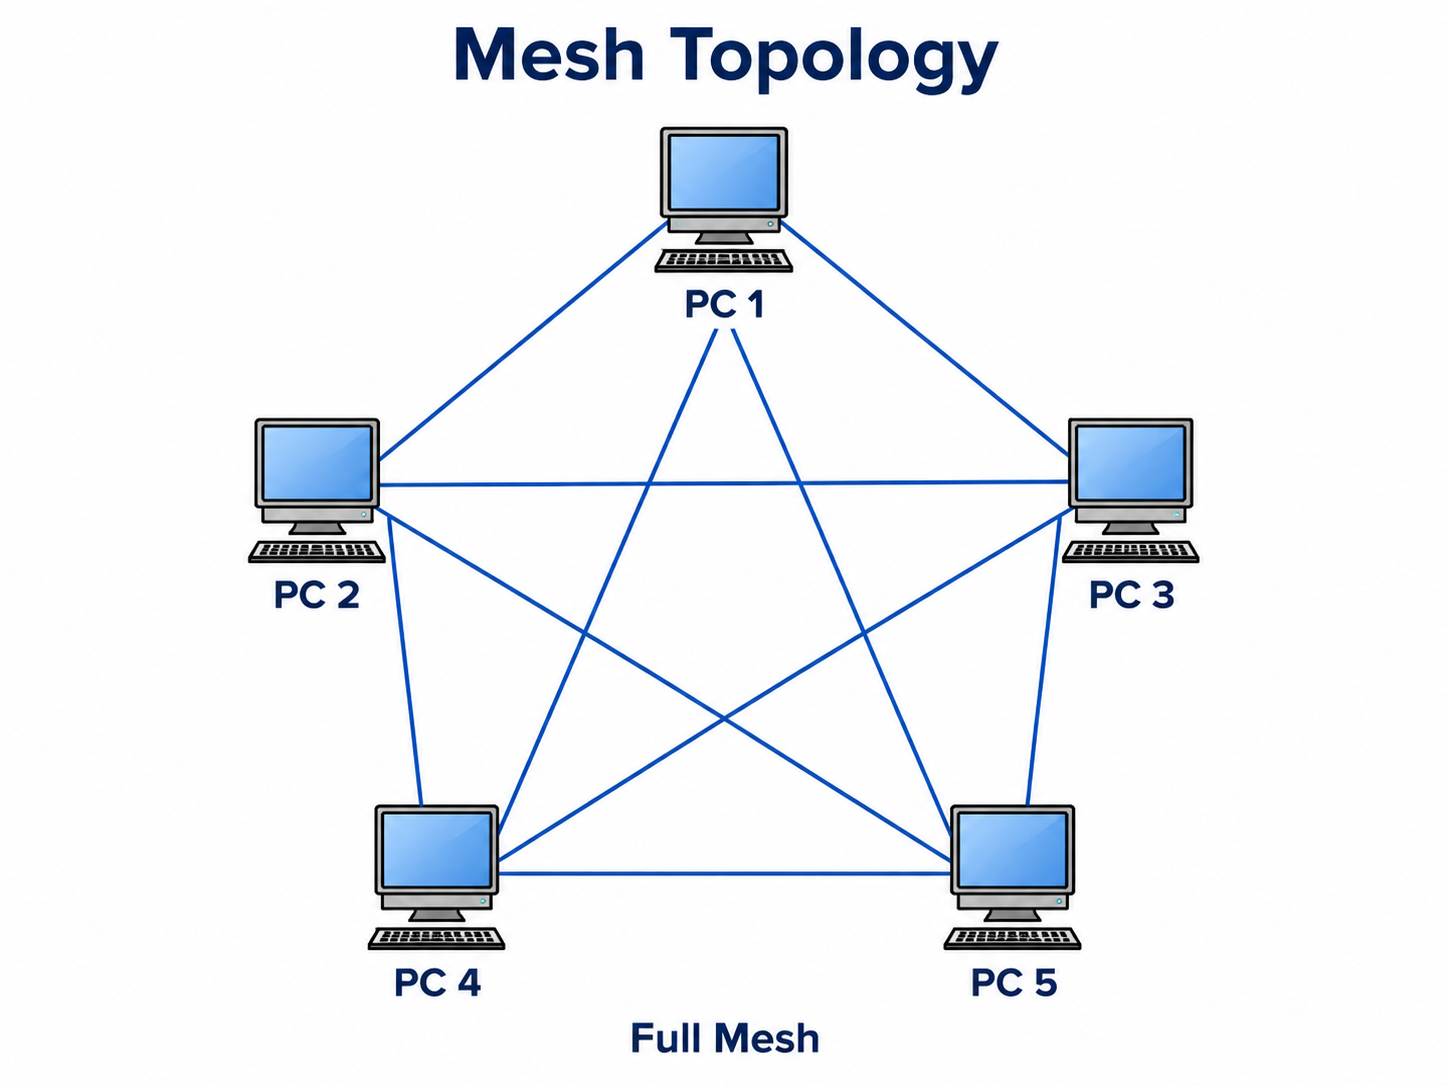
\includegraphics[width=0.86\textwidth]{chapters/Chapter02/images/mesh_topology_diagram.png}
}{
\fbox{
\parbox{0.84\textwidth}{
\centering
\vspace{0.7cm}
PC 1 \quad \rule{2cm}{0.5pt} \quad PC 2[8pt]
|\diagdown \quad \diagup|[8pt]
|\diagup \quad \diagdown|[8pt]
PC 3 \quad \rule{2cm}{0.5pt} \quad PC 4[8pt]
Multiple Links
\vspace{0.7cm}
}}
}
\caption{Mesh topology}
\end{figure}

\begin{examplebox}{বাস্তব উদাহরণ}
High reliability দরকার এমন network, যেমন backbone network, military communication বা critical data center interconnection-এ mesh বা partial mesh design ব্যবহার করা যেতে পারে।
\end{examplebox}

\subsection{Mesh Topology-এর সুবিধা ও অসুবিধা}

\begin{center}
\begin{tabular}{|p{0.43\textwidth}|p{0.43\textwidth}|}
\hline
\textbf{সুবিধা} & \textbf{অসুবিধা} \
\hline
reliability খুব বেশি & cable ও port বেশি লাগে \
\hline
alternative path থাকে & installation cost বেশি \
\hline
fault tolerance ভালো & design ও maintenance complex \
\hline
এক link নষ্ট হলেও communication চলতে পারে & ছোট সাধারণ network-এর জন্য অতিরিক্ত ব্যয়বহুল \
\hline
\end{tabular}
\end{center}

\subsection{Tree Topology}

\begin{definitionbox}{Tree Topology}
যে topology-তে star topology-এর একাধিক group hierarchy বা tree structure আকারে connected থাকে, তাকে Tree topology বলা হয়।
\end{definitionbox}

Tree topology-তে root বা backbone level থাকে এবং তার নিচে branch আকারে বিভিন্ন star network connected থাকতে পারে। বড় school, college, office বা campus network বোঝাতে Tree topology useful।

\begin{keypointbox}{Tree topology-এর বৈশিষ্ট্য}
\begin{itemize}
\item hierarchical structure থাকে।
\item একাধিক star topology combine হতে পারে।
\item বড় network organize করা সহজ।
\item department বা floor-wise network design করা যায়।
\item backbone বা root device নষ্ট হলে বড় অংশ affected হতে পারে।
\item cable ও device planning দরকার হয়।
\end{itemize}
\end{keypointbox}

\begin{figure}[H]
\centering
\IfFileExists{chapters/Chapter02/images/tree_topology_diagram.png}{
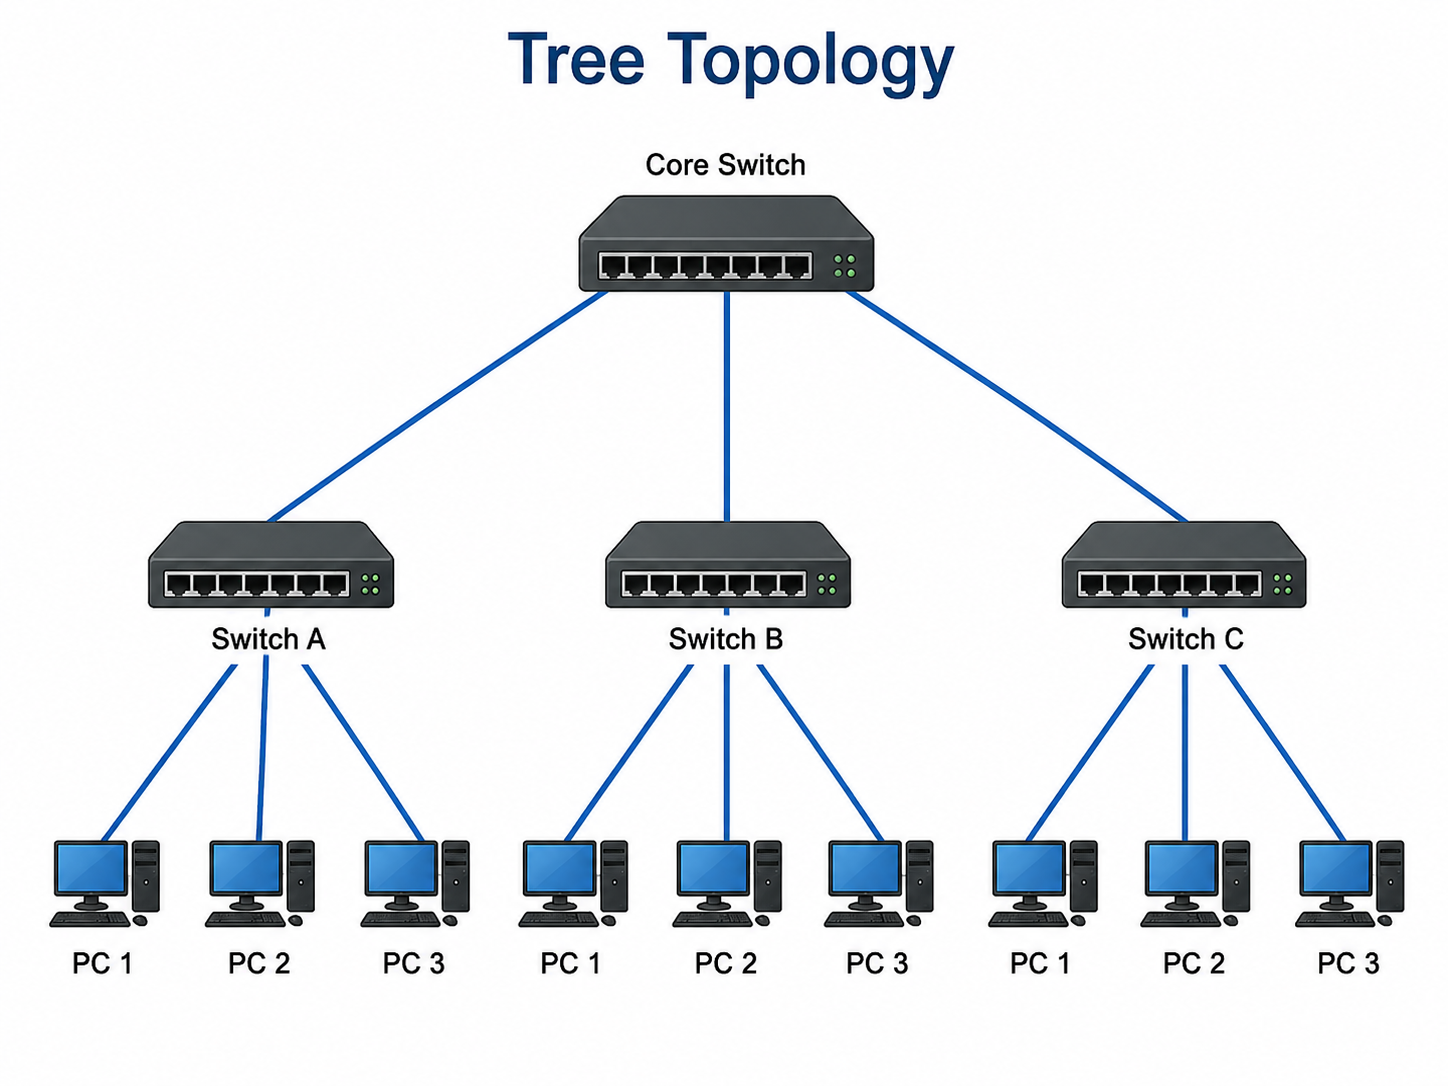
\includegraphics[width=0.90\textwidth]{chapters/Chapter02/images/tree_topology_diagram.png}
}{
\fbox{
\parbox{0.88\textwidth}{
\centering
\vspace{0.7cm}
Core Switch[8pt]
$\swarrow$ \quad $\downarrow$ \quad $\searrow$[8pt]
Switch A \quad Switch B \quad Switch C[8pt]
$\downarrow$ \quad \quad $\downarrow$ \quad \quad $\downarrow$[8pt]
PC Group A \quad PC Group B \quad PC Group C
\vspace{0.7cm}
}}
}
\caption{Tree topology}
\end{figure}

\begin{examplebox}{বাস্তব উদাহরণ}
একটি কলেজের admin building, ICT lab ও library-এর network আলাদা switch-এ connected, আর সব switch একটি core switch-এর সাথে connected—এটি Tree topology দিয়ে বোঝানো যায়।
\end{examplebox}

\subsection{Tree Topology-এর সুবিধা ও অসুবিধা}

\begin{center}
\begin{tabular}{|p{0.43\textwidth}|p{0.43\textwidth}|}
\hline
	\textbf{সুবিধা} & \textbf{অসুবিধা} \\
\hline
বড় network manage করা সহজ & backbone/root failure বড় অংশকে প্রভাবিত করতে পারে \\
\hline
department-wise network করা যায় & cable ও device বেশি লাগে \\
\hline
scalable, অর্থাৎ node add করা সহজ & configuration ও maintenance complex হতে পারে \\
\hline
fault isolation কিছুটা সহজ & cost তুলনামূলক বেশি \\
\hline
\end{tabular}
\end{center}

\subsection{Hybrid Topology}

\begin{definitionbox}{Hybrid Topology}
দুই বা ততোধিক topology একত্রে ব্যবহার করে যে network topology তৈরি হয়, তাকে Hybrid topology বলা হয়।
\end{definitionbox}

বাস্তব বড় network-এ অনেক সময় একটি topology যথেষ্ট হয় না। যেমন একটি campus network-এ computer lab-এ Star topology, building-to-building connection-এ Mesh/Tree concept এবং wireless area-তে access point-based star structure থাকতে পারে। এই combination-ই Hybrid topology।

\begin{keypointbox}{Hybrid topology-এর বৈশিষ্ট্য}
\begin{itemize}
\item একাধিক topology combine করে তৈরি হয়।
\item বাস্তব বড় network design-এ বেশি ব্যবহারযোগ্য।
\item flexibility বেশি।
\item performance ও reliability requirement অনুযায়ী design করা যায়।
\item design, installation ও maintenance complex।
\item cost তুলনামূলক বেশি হতে পারে।
\end{itemize}
\end{keypointbox}

\begin{figure}[H]
\centering
\IfFileExists{chapters/Chapter02/images/hybrid_topology_diagram.png}{
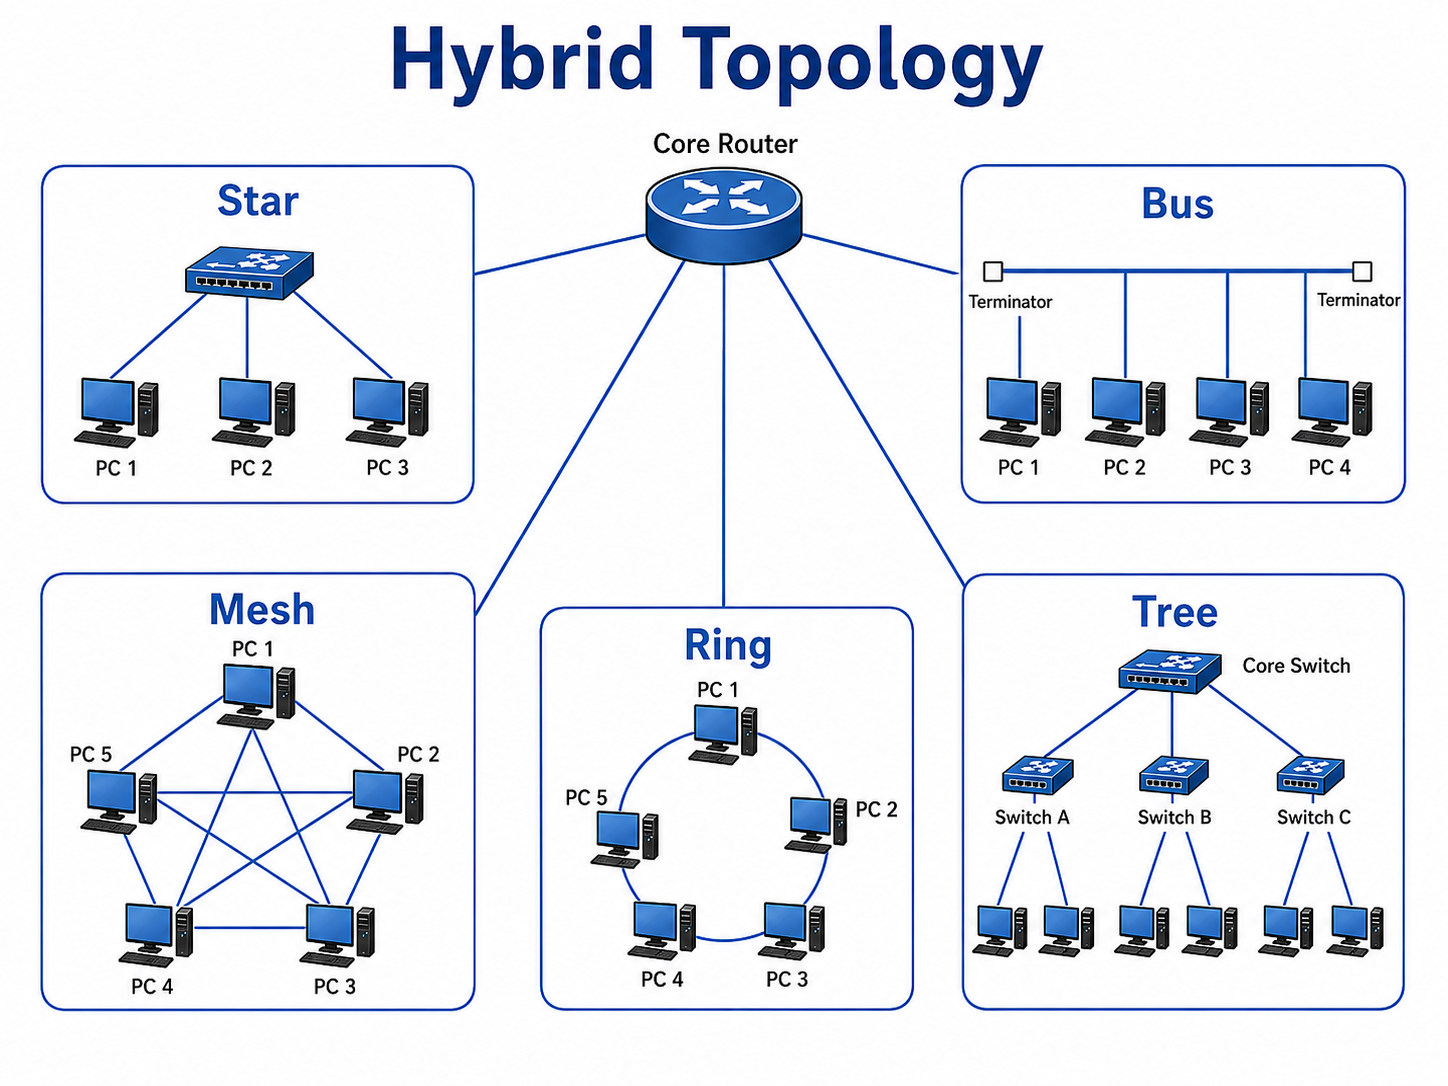
\includegraphics[width=0.92\textwidth]{chapters/Chapter02/images/hybrid_topology_diagram.png}
}{
\fbox{
\parbox{0.90\textwidth}{
\centering
\vspace{0.7cm}
Star Group A \quad $\longleftrightarrow$ \quad Core Router/Switch \quad $\longleftrightarrow$ \quad Star Group B[8pt]
Mesh/Tree Backbone + Star LAN Groups
\vspace{0.7cm}
}}
}
\caption{Hybrid topology}
\end{figure}

\begin{examplebox}{বাস্তব উদাহরণ}
একটি university campus network-এ প্রতিটি department star topology ব্যবহার করতে পারে, আবার department switches গুলো core network-এর সাথে tree/hybrid structure-এ connected থাকতে পারে।
\end{examplebox}

\subsection{প্রধান Topology-গুলোর তুলনা}

\begin{center}
\begin{tabular}{|p{0.16\textwidth}|p{0.23\textwidth}|p{0.22\textwidth}|p{0.22\textwidth}|}
\hline
\textbf{Topology} & \textbf{Structure} & \textbf{সুবিধা} & \textbf{অসুবিধা} \
\hline
Bus & common backbone cable & cost কম, সহজ setup & backbone failure-এ network বন্ধ \
\hline
Star & central switch/hub & manage ও troubleshoot সহজ & central device failure risky \
\hline
Ring & closed loop & ordered data flow & node/link failure problem \
\hline
Mesh & multiple interconnection & reliability বেশি & cost ও complexity বেশি \
\hline
Tree & hierarchical structure & বড় network organize সহজ & backbone/root dependency \
\hline
Hybrid & mixed topology & flexible ও practical & design complex, cost বেশি \
\hline
\end{tabular}
\end{center}

\begin{figure}[H]
\centering
\IfFileExists{chapters/Chapter02/images/network_topology_comparison_chart.png}{
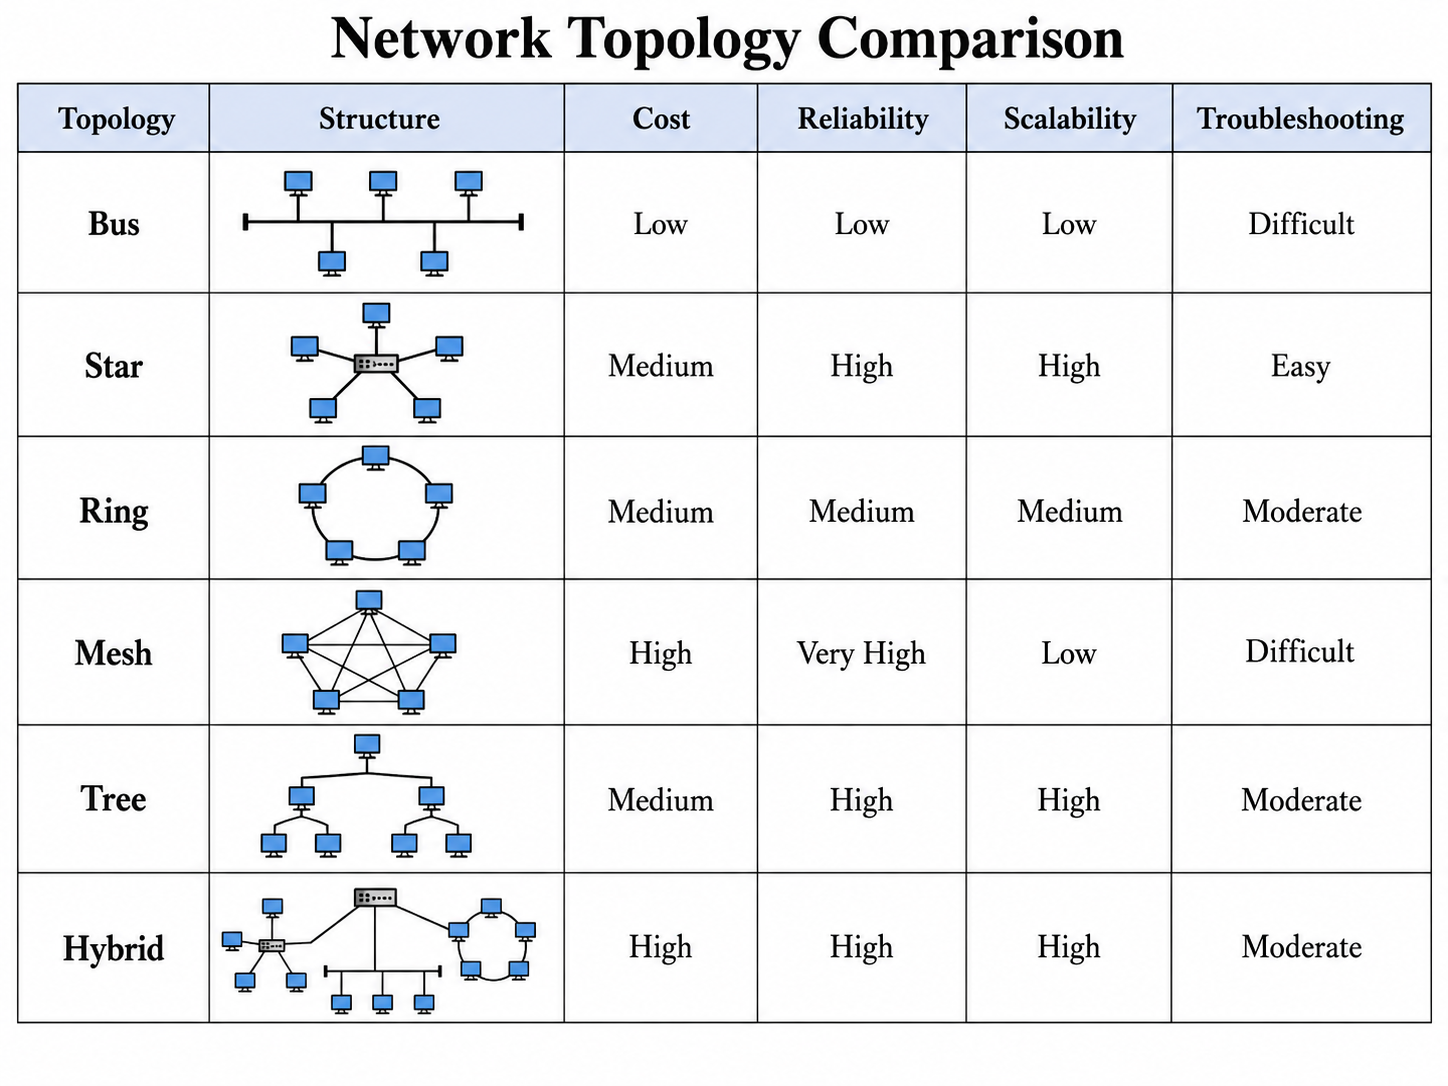
\includegraphics[width=0.94\textwidth]{chapters/Chapter02/images/network_topology_comparison_chart.png}
}{
\fbox{
\parbox{0.92\textwidth}{
\centering
\vspace{0.7cm}
Bus \quad Star \quad Ring \quad Mesh \quad Tree \quad Hybrid[8pt]
Cost \quad Reliability \quad Scalability \quad Troubleshooting
\vspace{0.7cm}
}}
}
\caption{নেটওয়ার্ক টপোলজির তুলনা}
\end{figure}

\subsection{কোন পরিস্থিতিতে কোন topology ব্যবহার হবে?}

\begin{center}
\begin{tabular}{|p{0.34\textwidth}|p{0.24\textwidth}|p{0.30\textwidth}|}
\hline
\textbf{পরিস্থিতি} & \textbf{উপযুক্ত topology} & \textbf{কারণ} \
\hline
ছোট পুরনো বা temporary network & Bus & cable কম লাগে, setup সহজ \
\hline
School computer lab & Star & switch দিয়ে device manage সহজ \
\hline
ordered data flow দরকার এমন controlled network & Ring & data নির্দিষ্ট path ধরে যায় \
\hline
high reliability critical network & Mesh & alternative path থাকে \
\hline
বড় office বা campus network & Tree & hierarchy অনুযায়ী network organize করা যায় \
\hline
university/corporate mixed network & Hybrid & বিভিন্ন requirement অনুযায়ী topology mix করা যায় \
\hline
\end{tabular}
\end{center}

\begin{figure}[H]
\centering
\IfFileExists{chapters/Chapter02/images/topology_selection_scenario.png}{
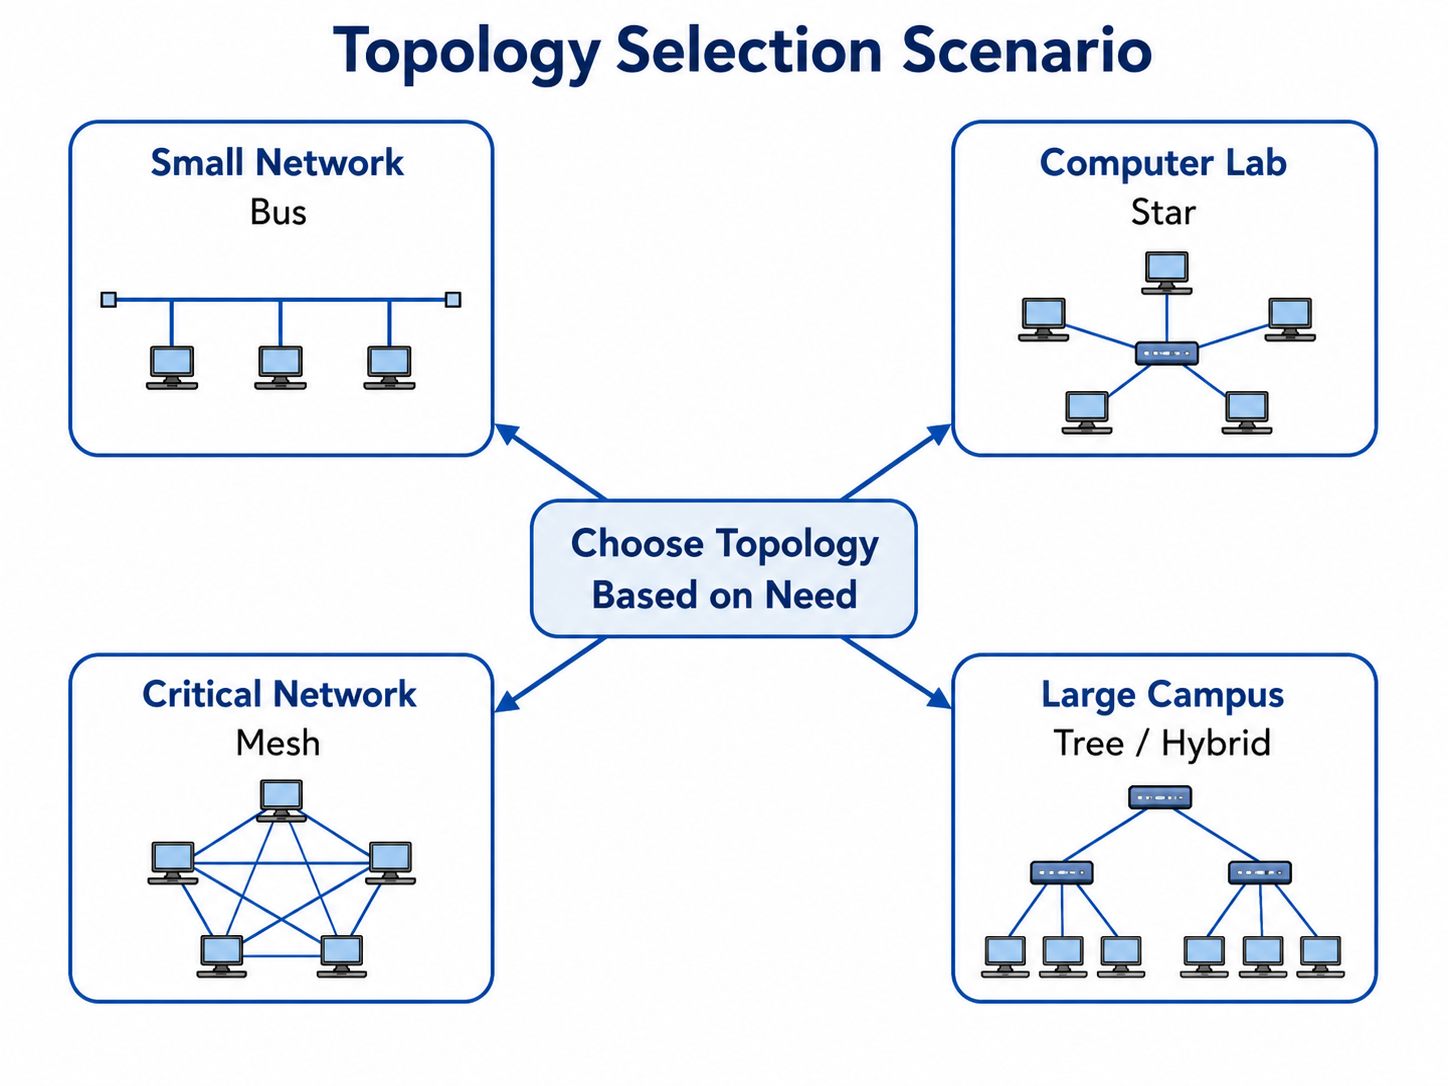
\includegraphics[width=0.92\textwidth]{chapters/Chapter02/images/topology_selection_scenario.png}
}{
\fbox{
\parbox{0.90\textwidth}{
\centering
\vspace{0.7cm}
Small Lab: Star[6pt]
Campus: Tree / Hybrid[6pt]
Critical Backbone: Mesh[6pt]
Temporary Network: Bus
\vspace{0.7cm}
}}
}
\caption{পরিস্থিতি অনুযায়ী topology নির্বাচন}
\end{figure}

\subsection{Topology নির্বাচন করার সময় বিবেচ্য বিষয়}

সব network-এর জন্য একই topology best নয়। ব্যবহার, budget, reliability, security, future expansion এবং maintenance facility অনুযায়ী topology নির্বাচন করতে হয়।

\begin{keypointbox}{Topology selection factors}
\begin{itemize}
\item \textbf{Network size}: node সংখ্যা কত?
\item \textbf{Cost}: cable, switch, router ও installation cost কত?
\item \textbf{Reliability}: কোনো link/device নষ্ট হলে network বন্ধ হওয়া যাবে কি না?
\item \textbf{Scalability}: ভবিষ্যতে নতুন device যোগ করা লাগবে কি?
\item \textbf{Performance}: data traffic কত বেশি?
\item \textbf{Troubleshooting}: fault খুঁজে বের করা সহজ কি?
\item \textbf{Security}: data path কতটা controlled?
\item \textbf{Maintenance}: network maintain করার দক্ষতা ও resource আছে কি?
\end{itemize}
\end{keypointbox}

\subsection{Common Mistake Zone}

\begin{mistakebox}{Common mistake ১}
অনেকে topology ও network type গুলিয়ে ফেলে। LAN, MAN, WAN হলো area অনুযায়ী network type; Bus, Star, Ring, Mesh ইত্যাদি হলো topology বা connection layout।
\end{mistakebox}

\begin{mistakebox}{Common mistake ২}
Star topology-তে central device থাকলেই সবসময় router হবে—এটি ঠিক নয়। সাধারণ LAN-এ central device হিসেবে switch বেশি ব্যবহৃত হয়।
\end{mistakebox}

\begin{mistakebox}{Common mistake ৩}
Mesh topology মানেই সবসময় full mesh নয়। Partial mesh-ও হতে পারে, যেখানে শুধু গুরুত্বপূর্ণ node-গুলো multiple link দিয়ে connected থাকে।
\end{mistakebox}

\begin{mistakebox}{Common mistake ৪}
Bus topology-তে কোনো central switch থাকে না; একটি common backbone cable থাকে। Star topology-তে central switch/hub থাকে।
\end{mistakebox}

\subsection{Exam-style প্রশ্ন ও উত্তর}

\begin{boardbox}{সংক্ষিপ্ত প্রশ্ন: Network topology কী?}
কম্পিউটার নেটওয়ার্কে computer, server, switch, router, printer ইত্যাদি node বা device কীভাবে পরস্পরের সাথে যুক্ত ও বিন্যস্ত থাকে, সেই physical বা logical arrangement-কে network topology বলা হয়। যেমন—Bus, Star, Ring, Mesh, Tree ও Hybrid topology।
\end{boardbox}

\begin{boardbox}{সংক্ষিপ্ত প্রশ্ন: Bus topology কী?}
যে network topology-তে সব node একটি common communication line বা backbone cable-এর সাথে যুক্ত থাকে, তাকে Bus topology বলা হয়। এতে cable কম লাগে, কিন্তু backbone cable নষ্ট হলে পুরো network বন্ধ হতে পারে।
\end{boardbox}

\begin{boardbox}{সংক্ষিপ্ত প্রশ্ন: Star topology কী?}
যে network topology-তে সব node একটি central device যেমন switch বা hub-এর সাথে আলাদাভাবে connected থাকে, তাকে Star topology বলা হয়। আধুনিক LAN ও computer lab network-এ এটি বেশি ব্যবহৃত হয়।
\end{boardbox}

\begin{boardbox}{সংক্ষিপ্ত প্রশ্ন: Ring topology কী?}
যে network topology-তে প্রতিটি node তার পাশের দুইটি node-এর সাথে connected থাকে এবং সব node মিলে closed loop বা ring তৈরি করে, তাকে Ring topology বলা হয়। এতে data সাধারণত নির্দিষ্ট direction-এ node থেকে node-এ যায়।
\end{boardbox}

\begin{boardbox}{সংক্ষিপ্ত প্রশ্ন: Mesh topology কী?}
যে topology-তে প্রতিটি node অন্য node-গুলোর সাথে সরাসরি বা একাধিক path দ্বারা connected থাকে, তাকে Mesh topology বলা হয়। এতে reliability বেশি, কিন্তু cable ও cost বেশি লাগে।
\end{boardbox}

\begin{boardbox}{সংক্ষিপ্ত প্রশ্ন: Tree topology কী?}
যে topology-তে star topology-এর একাধিক group hierarchy বা tree structure আকারে connected থাকে, তাকে Tree topology বলা হয়। বড় office, school বা campus network organize করতে এটি ব্যবহারযোগ্য।
\end{boardbox}

\begin{boardbox}{সংক্ষিপ্ত প্রশ্ন: Hybrid topology কী?}
দুই বা ততোধিক topology একত্রে ব্যবহার করে যে network topology তৈরি হয়, তাকে Hybrid topology বলা হয়। বড় বাস্তব network-এ বিভিন্ন requirement পূরণের জন্য hybrid topology ব্যবহার করা হয়।
\end{boardbox}

\begin{boardbox}{পার্থক্য: Bus ও Star topology}
Bus topology-তে সব node একটি common backbone cable-এর সাথে connected থাকে। Backbone cable নষ্ট হলে পুরো network বন্ধ হতে পারে। অন্যদিকে Star topology-তে সব node একটি central switch/hub-এর সাথে connected থাকে। এখানে একটি node বা cable নষ্ট হলে সাধারণত শুধু সেই node affected হয়, কিন্তু central device নষ্ট হলে network বন্ধ হতে পারে।
\end{boardbox}

\begin{boardbox}{পার্থক্য: Star ও Mesh topology}
Star topology-তে সব node central device-এর সাথে connected থাকে, তাই management সহজ কিন্তু central device-এর উপর dependency থাকে। Mesh topology-তে multiple link ও alternative path থাকে, তাই reliability বেশি; তবে cable, port, cost ও configuration complexity বেশি।
\end{boardbox}

\subsection{Brainstorming Critical Question}

\begin{practicebox}
একটি কলেজে ৩টি building আছে—Admin building, ICT lab এবং Library। ICT lab-এ ৩০টি computer আছে। Principal চান lab network সহজে manage করা যাবে, building গুলোর মধ্যে reliable connection থাকবে এবং ভবিষ্যতে নতুন department add করা যাবে।

\begin{enumerate}
\item ক. Network topology কী?
\item খ. Star topology computer lab-এর জন্য উপযোগী কেন?
\item গ. ICT lab-এর ৩০টি computer connect করতে কোন topology ব্যবহার করা যুক্তিযুক্ত? ব্যাখ্যা কর।
\item ঘ. পুরো কলেজ campus network-এর জন্য Tree/Hybrid topology কেন বেশি উপযোগী হতে পারে? বিশ্লেষণ কর।
\end{enumerate}
\end{practicebox}

\subsection{১ মিনিটে রিভিশন}

\begin{recapbox}
\begin{itemize}
\item Network topology হলো network device বা node-এর arrangement।
\item Physical topology device ও cable-এর বাস্তব layout বোঝায়।
\item Logical topology data flow path বোঝায়।
\item Bus topology-তে common backbone cable থাকে।
\item Star topology-তে central switch/hub থাকে।
\item Ring topology-তে node-গুলো closed loop তৈরি করে।
\item Mesh topology-তে multiple path থাকে এবং reliability বেশি।
\item Tree topology hierarchical structure তৈরি করে।
\item Hybrid topology দুই বা ততোধিক topology-এর combination।
\item School lab-এর জন্য Star topology বেশি ব্যবহারযোগ্য।
\item Campus network-এর জন্য Tree বা Hybrid topology উপযোগী।
\item Critical network-এর জন্য Mesh topology reliable।
\end{itemize}
\end{recapbox}

\subsection{অনুশীলন}

\begin{practicebox}
\textbf{MCQ}

\begin{enumerate}
\item Network topology কী নির্দেশ করে?\
ক. monitor-এর size \quad খ. device/node-এর arrangement \quad গ. printer-এর speed \quad ঘ. keyboard layout

\item Bus topology-তে সব node কিসের সাথে connected থাকে?\
ক. central switch \quad খ. backbone cable \quad গ. satellite \quad ঘ. scanner

\item Star topology-তে central device হিসেবে সাধারণত কোনটি ব্যবহৃত হয়?\
ক. Switch \quad খ. Keyboard \quad গ. Speaker \quad ঘ. Scanner

\item কোন topology-তে node-গুলো closed loop তৈরি করে?\
ক. Bus \quad খ. Star \quad গ. Ring \quad ঘ. Tree

\item কোন topology-তে reliability বেশি কিন্তু cost বেশি?\
ক. Mesh \quad খ. Bus \quad গ. Simplex \quad ঘ. Modem

\item Tree topology-এর structure কেমন?\
ক. linear \quad খ. hierarchical \quad গ. circular only \quad ঘ. no link

\item দুই বা ততোধিক topology মিলে কোন topology তৈরি হয়?\
ক. Hybrid \quad খ. Bus \quad গ. Ring \quad ঘ. NIC

\item School computer lab-এর জন্য সাধারণত কোন topology বেশি উপযোগী?\
ক. Star \quad খ. Bus only \quad গ. Ring only \quad ঘ. None
\end{enumerate}

\textbf{উত্তরমালা:}
১. খ, ২. খ, ৩. ক, ৪. গ, ৫. ক, ৬. খ, ৭. ক, ৮. ক

\vspace{0.3cm}

\textbf{সংক্ষিপ্ত প্রশ্ন}
\begin{enumerate}
\item Network topology কী?
\item Physical topology ও Logical topology-এর পার্থক্য লেখ।
\item Bus topology-এর বৈশিষ্ট্য লেখ।
\item Star topology কেন computer lab-এর জন্য উপযোগী?
\item Ring topology-এর একটি সুবিধা ও একটি অসুবিধা লেখ।
\item Mesh topology কেন reliable?
\item Tree topology কোথায় ব্যবহার করা যায়?
\item Hybrid topology বলতে কী বোঝায়?
\item Bus ও Star topology-এর মধ্যে পার্থক্য লেখ।
\item topology নির্বাচন করার সময় কোন কোন বিষয় বিবেচনা করতে হয়?
\end{enumerate}

\textbf{সৃজনশীল প্রশ্ন}
একটি hospital network-এ emergency department, pathology lab, billing section এবং server room আছে। প্রতিটি section-এর computer একটি local switch-এর সাথে যুক্ত। সব switch আবার server room-এর core switch-এর সাথে connected। Hospital authority চায় network expandable, manageable এবং reliable হোক।

\begin{enumerate}
\item ক. Star topology কী?
\item খ. Mesh topology reliable কেন?
\item গ. প্রতিটি section-এর computer connect করতে কোন topology ব্যবহার করা হয়েছে? ব্যাখ্যা কর।
\item ঘ. পুরো hospital network-এর জন্য Tree/Hybrid topology ব্যবহার যুক্তিযুক্ত কি না—বিশ্লেষণ কর।
\end{enumerate}
\end{practicebox}

% Chapter 02.10: Cloud computing basics
\section{Cloud Computing}

\subsection{Cloud Overview}
\begin{itemize}
\item Definition of cloud computing
\item On-demand resource provisioning
\end{itemize}

\subsection{Service Models}
\begin{itemize}
\item IaaS, PaaS, SaaS
\item উদাহরণ ও ব্যবহারক্ষেত্র
\end{itemize}

\subsection{Deployment Models}
\begin{itemize}
\item Public, Private, Hybrid, Community
\end{itemize}

% Chapter 02.11: অধ্যায়ভিত্তিক অনুশীলন
\section{অধ্যায়ভিত্তিক অনুশীলন: কমিউনিকেশন সিস্টেম ও নেটওয়ার্কিং}

\begin{learningbox}
এই অনুশীলন অংশ শেষে শিক্ষার্থী পারবে:
\begin{itemize}
\item Chapter 02-এর গুরুত্বপূর্ণ সব topic একসাথে revise করতে।
\item MCQ, short question ও creative question-এর board-standard উত্তর লিখতে।
\item data communication, transmission mode, medium, wireless technology, network, network devices, topology ও cloud computing থেকে প্রশ্ন solve করতে।
\item scenario-based CQ-তে topic identify করে ব্যাখ্যা, বিশ্লেষণ ও মূল্যায়ন করতে।
\item পরীক্ষার আগে দ্রুত final revision নিতে।
\end{itemize}
\end{learningbox}

\subsection{অধ্যায় ০২: গুরুত্বপূর্ণ Topic List}

\begin{keypointbox}{যে topicগুলো থেকে প্রশ্ন বেশি হয়}
\begin{itemize}
\item Data communication system ও এর উপাদান
\item Data transmission method: asynchronous, synchronous, isochronous
\item Data transmission mode: simplex, half-duplex, full-duplex
\item Data delivery mode: unicast, broadcast, multicast
\item Data communication medium: guided ও unguided media
\item Twisted pair, coaxial cable, optical fiber
\item Radio wave, microwave, infrared, satellite communication
\item Wi-Fi, Bluetooth, WiMAX
\item Mobile communication, handoff, roaming, mobile generation
\item Computer network, PAN, LAN, MAN, WAN
\item Client-server ও peer-to-peer network
\item Internet, intranet, extranet
\item Network devices: NIC, modem, hub, switch, router, bridge, gateway, repeater, access point, firewall
\item Network topology: bus, star, ring, mesh, tree, hybrid
\item Cloud computing: characteristics, service model, deployment model, advantages, disadvantages, security
\end{itemize}
\end{keypointbox}

\subsection{১ মিনিটে Full Chapter Revision}

\begin{recapbox}
\begin{itemize}
\item Data communication হলো এক device থেকে অন্য device-এ data পাঠানোর প্রক্রিয়া।
\item Sender, receiver, message, medium ও protocol হলো data communication-এর প্রধান উপাদান।
\item Transmission mode data কোন direction-এ যাবে তা বোঝায়।
\item Simplex একমুখী, half-duplex দুইমুখী কিন্তু একসাথে নয়, full-duplex দুইমুখী ও একই সময়ে।
\item Guided media physical cable ব্যবহার করে; unguided media wireless wave ব্যবহার করে।
\item Optical fiber light signal ব্যবহার করে high-speed data transmission করে।
\item Radio wave mobile, Wi-Fi ও Bluetooth communication-এ ব্যবহৃত হয়।
\item Computer network resource sharing, communication ও data sharing সহজ করে।
\item LAN ছোট area, MAN city-level area, WAN large geographical area cover করে।
\item Switch MAC address দেখে data forward করে; router network-to-network data path নির্ধারণ করে।
\item Hub data broadcast করে, switch নির্দিষ্ট destination-এ data পাঠায়।
\item Topology হলো network device বা node-এর arrangement।
\item Star topology-তে central switch/hub থাকে; bus topology-তে backbone cable থাকে।
\item Mesh topology reliable, কারণ multiple path থাকে।
\item Cloud computing হলো internet-এর মাধ্যমে remote server, storage, software ও computing resource ব্যবহার।
\item IaaS infrastructure, PaaS platform, SaaS ready software service দেয়।
\item Public cloud shared, private cloud dedicated, hybrid cloud public ও private cloud-এর combination।
\end{itemize}
\end{recapbox}

\subsection{Board Focus Short Notes}

\begin{boardbox}{প্রশ্ন: Data communication system-এর উপাদানগুলো কী কী?}
Data communication system-এর প্রধান উপাদান হলো sender, receiver, message, transmission medium এবং protocol। Sender data পাঠায়, receiver data গ্রহণ করে, message হলো পাঠানো data, medium হলো data চলাচলের path এবং protocol হলো communication-এর rules।
\end{boardbox}

\begin{boardbox}{প্রশ্ন: Full-duplex mode কেন বেশি কার্যকর?}
Full-duplex mode-এ sender ও receiver একই সময়ে data পাঠাতে ও গ্রহণ করতে পারে। ফলে communication দ্রুত ও কার্যকর হয়। Telephone, mobile phone ও video call full-duplex communication-এর উদাহরণ।
\end{boardbox}

\begin{boardbox}{প্রশ্ন: Optical fiber কেন high-speed communication-এ ব্যবহৃত হয়?}
Optical fiber light signal ব্যবহার করে data পাঠায়। এতে bandwidth বেশি, long distance communication সম্ভব এবং electromagnetic interference-এর প্রভাব কম। তাই internet backbone, FTTH broadband ও data center connection-এ optical fiber ব্যবহৃত হয়।
\end{boardbox}

\begin{boardbox}{প্রশ্ন: Switch ও Hub-এর মধ্যে পার্থক্য কী?}
Hub কোনো data পেলে সেটি সব port-এ broadcast করে। কিন্তু switch MAC address table ব্যবহার করে data নির্দিষ্ট destination port-এ forward করে। তাই switch hub-এর তুলনায় efficient, secure এবং collision কম হয়।
\end{boardbox}

\begin{boardbox}{প্রশ্ন: Router-এর কাজ কী?}
Router এক network-কে অন্য network-এর সাথে connect করে এবং data packet কোন route দিয়ে destination network-এ যাবে তা নির্ধারণ করে। Internet connection ও LAN-to-WAN communication-এ router গুরুত্বপূর্ণ device।
\end{boardbox}

\begin{boardbox}{প্রশ্ন: Star topology computer lab-এর জন্য উপযোগী কেন?}
Star topology-তে সব computer central switch বা hub-এর সাথে connected থাকে। নতুন computer add করা সহজ, fault finding সহজ এবং একটি computer বা cable নষ্ট হলে সাধারণত পুরো network বন্ধ হয় না। তাই school বা college computer lab-এর জন্য star topology উপযোগী।
\end{boardbox}

\begin{boardbox}{প্রশ্ন: Cloud computing-এর সুবিধা কী?}
Cloud computing-এর মাধ্যমে internet ব্যবহার করে remote server, storage ও software service ব্যবহার করা যায়। এতে hardware cost কমে, scalability বাড়ে, যেকোনো জায়গা থেকে access করা যায়, backup রাখা সহজ হয় এবং collaboration করা সহজ হয়।
\end{boardbox}

\subsection{MCQ: Board Standard Practice}

\begin{practicebox}
\textbf{নির্দেশনা: প্রতিটি প্রশ্নের সঠিক উত্তর নির্বাচন কর।}

\begin{enumerate}
\item Data communication বলতে কী বোঝায়?\
ক. শুধু data সংরক্ষণ \quad খ. data প্রেরণ ও গ্রহণ \quad গ. শুধু data delete \quad ঘ. monitor display

\item Data communication system-এ rules বা নিয়মকে কী বলা হয়?\
ক. Medium \quad খ. Protocol \quad গ. Cable \quad ঘ. Printer

\item নিচের কোনটি data communication-এর উপাদান নয়?\
ক. Sender \quad খ. Receiver \quad গ. Protocol \quad ঘ. Scanner

\item Data transmission mode নির্দেশ করে—\
ক. data কোন direction-এ যাবে \quad খ. data কোথায় store হবে \quad গ. monitor-এর size \quad ঘ. keyboard layout

\item Television broadcasting কোন transmission mode-এর উদাহরণ?\
ক. Simplex \quad খ. Half-duplex \quad গ. Full-duplex \quad ঘ. Multiplex

\item Walkie-talkie communication কোন mode-এর উদাহরণ?\
ক. Simplex \quad খ. Half-duplex \quad গ. Full-duplex \quad ঘ. Broadcast only

\item Telephone conversation কোন mode-এর উদাহরণ?\
ক. Simplex \quad খ. Half-duplex \quad গ. Full-duplex \quad ঘ. Unicast

\item এক sender থেকে এক receiver-এ data পাঠানোকে কী বলে?\
ক. Broadcast \quad খ. Multicast \quad গ. Unicast \quad ঘ. Anycast

\item এক sender থেকে network-এর সব receiver-এ data পাঠানোকে কী বলে?\
ক. Unicast \quad খ. Broadcast \quad গ. Multicast \quad ঘ. Duplex

\item Guided media-তে data কোন মাধ্যমে যায়?\
ক. physical cable \quad খ. শুধু বাতাস \quad গ. light ছাড়া \quad ঘ. keyboard

\item নিচের কোনটি guided media?\
ক. Radio wave \quad খ. Microwave \quad গ. Optical fiber \quad ঘ. Infrared

\item নিচের কোনটি unguided media?\
ক. Coaxial cable \quad খ. Twisted pair \quad গ. Radio wave \quad ঘ. Fiber optic

\item Twisted pair cable সাধারণত কোন network-এ বেশি ব্যবহৃত হয়?\
ক. LAN \quad খ. Satellite only \quad গ. TV remote \quad ঘ. Bluetooth only

\item Optical fiber cable কোন signal ব্যবহার করে?\
ক. Sound signal \quad খ. Light signal \quad গ. Mechanical signal \quad ঘ. Magnetic signal only

\item TV remote সাধারণত কোন medium ব্যবহার করে?\
ক. Infrared \quad খ. Optical fiber \quad গ. Coaxial cable \quad ঘ. Twisted pair

\item Microwave communication-এর জন্য সাধারণত কোনটি গুরুত্বপূর্ণ?\
ক. Line-of-sight \quad খ. Paper storage \quad গ. Printer speed \quad ঘ. keyboard layout

\item Bluetooth সাধারণত কোন ধরনের network তৈরি করে?\
ক. PAN \quad খ. MAN \quad গ. WAN \quad ঘ. Internet backbone

\item Wi-Fi কোন standard family-এর সাথে সম্পর্কিত?\
ক. IEEE 802.11 \quad খ. IEEE 802.3 only \quad গ. ASCII \quad ঘ. Unicode

\item একটি building বা office-এর মধ্যে network সাধারণত কোন ধরনের?\
ক. LAN \quad খ. MAN \quad গ. WAN \quad ঘ. Satellite network

\item City-wide network সাধারণত কোন ধরনের?\
ক. PAN \quad খ. LAN \quad গ. MAN \quad ঘ. Bluetooth

\item বড় geographical area cover করা network কোনটি?\
ক. PAN \quad খ. LAN \quad গ. WAN \quad ঘ. Star

\item Client-server network-এ server-এর কাজ কী?\
ক. শুধু monitor চালানো \quad খ. service/resource provide করা \quad গ. cable twist করা \quad ঘ. keyboard control

\item নিচের কোনটি network device?\
ক. Switch \quad খ. Speaker only \quad গ. Keyboard only \quad ঘ. Mouse pad

\item NIC-এর কাজ কী?\
ক. computer-কে network-এ connect করা \quad খ. monitor bright করা \quad গ. paper print করা \quad ঘ. sound amplify করা

\item Modem-এর কাজ কী?\
ক. modulation ও demodulation \quad খ. শুধু printing \quad গ. keyboard input \quad ঘ. image editing

\item Hub data পেলে কী করে?\
ক. সব port-এ broadcast করে \quad খ. শুধু destination port-এ পাঠায় \quad গ. data delete করে \quad ঘ. cloud-এ store করে

\item Switch সাধারণত কোন address ব্যবহার করে forwarding করে?\
ক. MAC address \quad খ. house address \quad গ. postal code \quad ঘ. ISBN

\item Router কী connect করে?\
ক. network-to-network \quad খ. keyboard-to-monitor \quad গ. speaker-to-mouse \quad ঘ. scanner-to-paper

\item Repeater-এর কাজ কী?\
ক. signal regenerate করা \quad খ. software install করা \quad গ. file delete করা \quad ঘ. keyboard clean করা

\item Gateway-এর কাজ কী?\
ক. protocol conversion \quad খ. printer color change \quad গ. monitor setup \quad ঘ. hard disk format

\item Firewall-এর কাজ কী?\
ক. network traffic filtering \quad খ. cable twisting \quad গ. speaker output \quad ঘ. keyboard input

\item Network topology কী নির্দেশ করে?\
ক. node/device arrangement \quad খ. monitor size \quad গ. CPU brand \quad ঘ. file extension

\item Bus topology-তে সব node কিসের সাথে connected থাকে?\
ক. common backbone cable \quad খ. individual router only \quad গ. satellite dish \quad ঘ. scanner

\item Star topology-তে central device হিসেবে সাধারণত কোনটি থাকে?\
ক. Switch/Hub \quad খ. Keyboard \quad গ. Scanner \quad ঘ. Speaker

\item Ring topology-তে node-গুলো কী গঠন করে?\
ক. closed loop \quad খ. straight line only \quad গ. no link \quad ঘ. cloud storage

\item Mesh topology কেন reliable?\
ক. multiple path থাকে \quad খ. cable নেই \quad গ. only one node থাকে \quad ঘ. no connection থাকে

\item দুই বা ততোধিক topology মিলে কোন topology তৈরি হয়?\
ক. Hybrid \quad খ. Simplex \quad গ. Protocol \quad ঘ. Infrared

\item Cloud computing কীসের মাধ্যমে ব্যবহার করা হয়?\
ক. Internet \quad খ. only keyboard \quad গ. only printer \quad ঘ. offline chalkboard

\item Google Drive কোন service-এর উদাহরণ?\
ক. Cloud storage \quad খ. Scanner service \quad গ. Hub service \quad ঘ. Mouse service

\item SaaS-এর পূর্ণরূপ কী?\
ক. Software as a Service \quad খ. Storage as a Switch \quad গ. Server as Scanner \quad ঘ. System as Sound

\item IaaS প্রধানত কী provide করে?\
ক. Infrastructure \quad খ. Ready-made email only \quad গ. keyboard \quad ঘ. monitor

\item PaaS বেশি উপযোগী কার জন্য?\
ক. Developer \quad খ. Painter only \quad গ. Typist only \quad ঘ. Electrician

\item Public ও Private cloud একত্রে ব্যবহার করলে কোন cloud model হয়?\
ক. Hybrid cloud \quad খ. Ring cloud \quad গ. Bus cloud \quad ঘ. Simplex cloud

\item Cloud security বাড়াতে কোনটি ব্যবহার করা ভালো?\
ক. Strong password ও MFA \quad খ. weak password \quad গ. password share করা \quad ঘ. public login

\item Data transfer speed সাধারণত কোন এককে প্রকাশ করা হয়?\
ক. bps \quad খ. kg \quad গ. meter \quad ঘ. volt only

\item Bandwidth বেশি হলে কী হয়?\
ক. বেশি data transfer করা যায় \quad খ. monitor ছোট হয় \quad গ. keyboard slow হয় \quad ঘ. file delete হয়

\item Protocol-এর উদাহরণ কোনটি?\
ক. TCP/IP \quad খ. Monitor \quad গ. Speaker \quad ঘ. Scanner

\item Internet কী ধরনের network?\
ক. network of networks \quad খ. শুধু LAN \quad গ. শুধু PAN \quad ঘ. keyboard system

\item Intranet সাধারণত কারা ব্যবহার করে?\
ক. একটি organization-এর internal users \quad খ. পুরো public internet \quad গ. শুধু printer \quad ঘ. only scanner

\item Extranet কী?\
ক. controlled external accessসহ private network \quad খ. keyboard layout \quad গ. TV signal \quad ঘ. printer ink
\end{enumerate}

\textbf{উত্তরমালা:}\
১. খ, ২. খ, ৩. ঘ, ৪. ক, ৫. ক, ৬. খ, ৭. গ, ৮. গ, ৯. খ, ১০. ক,\
১১. গ, ১২. গ, ১৩. ক, ১৪. খ, ১৫. ক, ১৬. ক, ১৭. ক, ১৮. ক, ১৯. ক, ২০. গ,\
২১. গ, ২২. খ, ২৩. ক, ২৪. ক, ২৫. ক, ২৬. ক, ২৭. ক, ২৮. ক, ২৯. ক, ৩০. ক,\
৩১. ক, ৩২. ক, ৩৩. ক, ৩৪. ক, ৩৫. ক, ৩৬. ক, ৩৭. ক, ৩৮. ক, ৩৯. ক, ৪০. ক,\
৪১. ক, ৪২. ক, ৪৩. ক, ৪৪. ক, ৪৫. ক, ৪৬. ক, ৪৭. ক, ৪৮. ক, ৪৯. ক, ৫০. ক
\end{practicebox}

\subsection{Board Standard Short Questions}

\begin{practicebox}
\textbf{সংক্ষিপ্ত প্রশ্ন}

\begin{enumerate}
\item Data communication কী?
\item Data communication system-এর পাঁচটি উপাদান লেখ।
\item Protocol কী? উদাহরণ দাও।
\item Bandwidth বলতে কী বোঝায়?
\item Simplex, half-duplex ও full-duplex mode-এর পার্থক্য লেখ।
\item Unicast, broadcast ও multicast delivery mode-এর পার্থক্য লেখ।
\item Guided media ও unguided media কী?
\item Twisted pair cable-এর বৈশিষ্ট্য লেখ।
\item Optical fiber cable কেন গুরুত্বপূর্ণ?
\item Radio wave ও microwave-এর মধ্যে পার্থক্য লেখ।
\item Infrared কোথায় ব্যবহৃত হয়?
\item Satellite communication কী?
\item Wi-Fi, Bluetooth ও WiMAX-এর মধ্যে পার্থক্য লেখ।
\item Mobile handoff কী?
\item Roaming বলতে কী বোঝায়?
\item Computer network কী?
\item LAN, MAN ও WAN-এর পার্থক্য লেখ।
\item Client-server network কী?
\item Peer-to-peer network কী?
\item Internet, intranet ও extranet-এর পার্থক্য লেখ।
\item NIC-এর কাজ কী?
\item Modem-এর কাজ কী?
\item Hub ও Switch-এর মধ্যে পার্থক্য লেখ।
\item Router কীভাবে network connect করে?
\item Repeater ও bridge-এর কাজ লেখ।
\item Gateway কেন protocol conversion করে?
\item Firewall কেন গুরুত্বপূর্ণ?
\item Network topology কী?
\item Bus ও Star topology-এর পার্থক্য লেখ।
\item Mesh topology কেন reliable?
\item Tree topology কোথায় ব্যবহার করা যায়?
\item Hybrid topology কী?
\item Cloud computing কী?
\item Cloud storage কী?
\item IaaS, PaaS ও SaaS-এর পার্থক্য লেখ।
\item Public cloud ও Private cloud-এর পার্থক্য লেখ।
\item Hybrid cloud কেন ব্যবহার করা হয়?
\item Cloud computing-এর সুবিধা লেখ।
\item Cloud computing-এর অসুবিধা লেখ।
\item Cloud security practice লিখ।
\end{enumerate}
\end{practicebox}

\subsection{Board CQ Practice Set}

\begin{practicebox}
\textbf{CQ-1: Data Communication System}

একটি কলেজে online admission system চালু করা হলো। শিক্ষার্থী mobile দিয়ে form পূরণ করে submit করে। Form-এর data internet ব্যবহার করে college server-এ যায়। Server data গ্রহণ করে database-এ সংরক্ষণ করে। System-টি সঠিকভাবে কাজ করার জন্য নির্দিষ্ট communication rules follow করে।

\begin{enumerate}
\item ক. Data communication কী?
\item খ. Protocol কেন প্রয়োজন?
\item গ. উদ্দীপকে data communication system-এর উপাদানগুলো শনাক্ত কর।
\item ঘ. College online admission system-এ data communication system-এর গুরুত্ব বিশ্লেষণ কর।
\end{enumerate}

\textbf{উত্তর নির্দেশনা:}
\begin{itemize}
\item ক: Sender থেকে receiver-এ data পাঠানোর প্রক্রিয়া।
\item খ: Protocol communication-এর rules নির্ধারণ করে; sender ও receiver একই নিয়ম follow না করলে data বুঝতে সমস্যা হয়।
\item গ: sender = student mobile, receiver/server = college server, message = form data, medium = internet, protocol = communication rules.
\item ঘ: দ্রুত form submission, accurate data transfer, server storage, remote access, reduced paper work, reliable communication—এসব point লিখবে।
\end{itemize}
\end{practicebox}

\begin{practicebox}
\textbf{CQ-2: Transmission Mode}

একটি school-এ notice board display system, walkie-talkie security system এবং online video class system ব্যবহার করা হয়। Notice board-এ office থেকে notice পাঠানো হয়, কিন্তু board কোনো reply পাঠায় না। Security guards walkie-talkie দিয়ে কথা বলে, কিন্তু একই সময়ে দুইজন কথা বলতে পারে না। Online class-এ teacher ও student একই সময়ে কথা বলতে ও শুনতে পারে।

\begin{enumerate}
\item ক. Transmission mode কী?
\item খ. Full-duplex mode বেশি কার্যকর কেন?
\item গ. উদ্দীপকের তিনটি system কোন কোন transmission mode ব্যবহার করছে? ব্যাখ্যা কর।
\item ঘ. Education system-এ full-duplex communication-এর প্রয়োজনীয়তা মূল্যায়ন কর।
\end{enumerate}

\textbf{উত্তর নির্দেশনা:}
\begin{itemize}
\item ক: data কোন direction-এ transfer হয় তার ধরন।
\item খ: একই সময়ে data send ও receive করা যায়।
\item গ: notice board = simplex, walkie-talkie = half-duplex, online video class = full-duplex.
\item ঘ: live class, question-answer, interaction, feedback, discussion, remote learning—এসব point লিখবে।
\end{itemize}
\end{practicebox}

\begin{practicebox}
\textbf{CQ-3: Transmission Media}

একটি hospital-এর doctor chamber-এ desktop computerগুলো switch-এর সাথে cable দিয়ে connected। Server room থেকে central database high-speed fiber connection ব্যবহার করে। Waiting area-তে Wi-Fi দেওয়া হয়েছে। Emergency department-এ short-range remote control device ব্যবহার করা হয়।

\begin{enumerate}
\item ক. Transmission medium কী?
\item খ. Guided media ও unguided media-এর মূল পার্থক্য কী?
\item গ. উদ্দীপকে ব্যবহৃত guided ও unguided media শনাক্ত কর।
\item ঘ. Hospital database connection-এর জন্য optical fiber বেশি উপযোগী কি না—বিশ্লেষণ কর।
\end{enumerate}

\textbf{উত্তর নির্দেশনা:}
\begin{itemize}
\item ক: sender থেকে receiver-এ signal যাওয়ার path।
\item খ: guided media cable-based; unguided media wireless wave-based।
\item গ: desktop-switch cable = twisted pair/guided; fiber = guided; Wi-Fi = radio wave/unguided; remote control = infrared/unguided.
\item ঘ: high bandwidth, low interference, long distance, reliable, secure; তবে cost ও maintenance বেশি—এগুলো লিখবে।
\end{itemize}
\end{practicebox}

\begin{practicebox}
\textbf{CQ-4: Wireless Communication}

একটি campus-এ students mobile phone, Bluetooth headphone, Wi-Fi router এবং tower-based broadband wireless connection ব্যবহার করে। Mobile phone tower-এর সাথে communication করে, Bluetooth headphone স্বল্প দূরত্বে কাজ করে, Wi-Fi classroom area cover করে এবং broadband wireless system দূরবর্তী area-তে internet দেয়।

\begin{enumerate}
\item ক. Wireless communication কী?
\item খ. Bluetooth PAN তৈরি করে কেন?
\item গ. উদ্দীপকের Bluetooth, Wi-Fi ও tower-based wireless technology ব্যাখ্যা কর।
\item ঘ. Campus network-এ Wi-Fi ও WiMAX/long-range wireless technology একসাথে ব্যবহার যুক্তিযুক্ত কি না—বিশ্লেষণ কর।
\end{enumerate}

\textbf{উত্তর নির্দেশনা:}
\begin{itemize}
\item ক: physical cable ছাড়া electromagnetic wave ব্যবহার করে communication।
\item খ: Bluetooth স্বল্প দূরত্বে personal devices connect করে।
\item গ: Bluetooth = short range PAN, Wi-Fi = WLAN, tower-based wireless = wider range wireless broadband.
\item ঘ: Wi-Fi indoor/classroom coverage; long-range wireless campus/backbone/remote area coverage; cost, coverage, mobility, bandwidth point লিখবে।
\end{itemize}
\end{practicebox}

\begin{practicebox}
\textbf{CQ-5: Computer Network}

একটি coaching center-এ ২০টি computer, একটি printer, একটি file server এবং internet connection আছে। Students একই printer ব্যবহার করে, teachers file server-এ notes রাখে এবং সব computer internet ব্যবহার করে। Admin চান ভবিষ্যতে আরও computer add করা যাবে।

\begin{enumerate}
\item ক. Computer network কী?
\item খ. Resource sharing বলতে কী বোঝায়?
\item গ. উদ্দীপকে network ব্যবহারের উদ্দেশ্যগুলো ব্যাখ্যা কর।
\item ঘ. Coaching center-এর জন্য LAN ব্যবহার কতটা যুক্তিযুক্ত—বিশ্লেষণ কর।
\end{enumerate}

\textbf{উত্তর নির্দেশনা:}
\begin{itemize}
\item ক: একাধিক computer/device সংযুক্ত হয়ে data ও resource share করার system।
\item খ: printer, file, internet ইত্যাদি একাধিক user share করে।
\item গ: printer sharing, file sharing, internet sharing, communication, centralized storage.
\item ঘ: same building/limited area, speed, easy management, cost-effective, expansion possible—এসব point লিখবে।
\end{itemize}
\end{practicebox}

\begin{practicebox}
\textbf{CQ-6: Network Devices}

একটি school lab-এ সব computer একটি switch-এর সাথে connected। Internet connection-এর জন্য router ব্যবহৃত হয়। দূরের building-এ signal দুর্বল হওয়ায় repeater ব্যবহার করা হয়েছে। External attack ঠেকাতে firewall setup করা হয়েছে।

\begin{enumerate}
\item ক. Network device কী?
\item খ. Router কেন প্রয়োজন?
\item গ. উদ্দীপকে switch, router, repeater ও firewall-এর কাজ ব্যাখ্যা কর।
\item ঘ. School lab network নিরাপদ ও কার্যকর করতে এসব device-এর ভূমিকা মূল্যায়ন কর।
\end{enumerate}

\textbf{উত্তর নির্দেশনা:}
\begin{itemize}
\item ক: network connect, manage বা protect করতে ব্যবহৃত hardware device।
\item খ: router LAN-কে অন্য network/internet-এর সাথে connect করে এবং path নির্ধারণ করে।
\item গ: switch = local forwarding, router = network connection, repeater = signal regeneration, firewall = filtering/security.
\item ঘ: efficient data flow, internet access, long distance signal improvement, security protection, scalability—এসব point লিখবে।
\end{itemize}
\end{practicebox}

\begin{practicebox}
\textbf{CQ-7: Hub, Switch ও Router}

একটি ছোট office প্রথমে hub ব্যবহার করত। এতে data সব computer-এ চলে যেত এবং traffic বেশি ছিল। পরে switch ব্যবহার করায় data নির্দিষ্ট computer-এ যাচ্ছে। Office network-কে internet-এর সাথে যুক্ত করতে router ব্যবহার করা হলো।

\begin{enumerate}
\item ক. Hub কী?
\item খ. Switch hub-এর তুলনায় efficient কেন?
\item গ. উদ্দীপকে hub, switch ও router-এর কাজ তুলনা কর।
\item ঘ. Office network উন্নত করতে hub-এর পরিবর্তে switch ও router ব্যবহার কতটা যুক্তিযুক্ত—বিশ্লেষণ কর।
\end{enumerate}

\textbf{উত্তর নির্দেশনা:}
\begin{itemize}
\item ক: hub হলো central device যা data সব port-এ broadcast করে।
\item খ: switch MAC address ব্যবহার করে নির্দিষ্ট destination-এ data পাঠায়।
\item গ: hub = broadcast, switch = intelligent forwarding, router = network-to-network/internet connection.
\item ঘ: traffic কমে, collision কমে, speed বাড়ে, security বাড়ে, internet connectivity হয়।
\end{itemize}
\end{practicebox}

\begin{practicebox}
\textbf{CQ-8: Network Topology}

একটি ICT lab-এ ৩০টি computer একটি central switch-এর সাথে connected। অন্যদিকে university campus-এর বিভিন্ন department switch আবার core switch-এর সাথে hierarchy আকারে connected। Research server-এর মধ্যে multiple path রাখা হয়েছে যাতে একটি link নষ্ট হলেও communication বন্ধ না হয়।

\begin{enumerate}
\item ক. Network topology কী?
\item খ. Mesh topology reliable কেন?
\item গ. উদ্দীপকের ICT lab, campus network ও research server-এর topology শনাক্ত কর।
\item ঘ. বড় campus network-এর জন্য tree/hybrid topology ব্যবহার যুক্তিযুক্ত কি না—বিশ্লেষণ কর।
\end{enumerate}

\textbf{উত্তর নির্দেশনা:}
\begin{itemize}
\item ক: network node/device-এর arrangement।
\item খ: multiple path থাকায় একটি link নষ্ট হলেও alternative path থাকে।
\item গ: ICT lab = star, campus = tree, research server = mesh/partial mesh.
\item ঘ: department-wise structure, scalability, management, fault isolation, backbone dependency, cost—এসব point লিখবে।
\end{itemize}
\end{practicebox}

\begin{practicebox}
\textbf{CQ-9: Cloud Computing}

একটি college Google Drive-এ notes share করে, students Google Docs-এ assignment করে এবং admin result database secure server-এ রাখে। Online class platform cloud server ব্যবহার করে, যাতে বেশি student login করলে resource বাড়ানো যায়।

\begin{enumerate}
\item ক. Cloud computing কী?
\item খ. Cloud storage শিক্ষার্থীদের জন্য সুবিধাজনক কেন?
\item গ. উদ্দীপকে SaaS ও cloud storage service শনাক্ত কর।
\item ঘ. College management system-এ hybrid cloud ব্যবহার যুক্তিযুক্ত কি না—বিশ্লেষণ কর।
\end{enumerate}

\textbf{উত্তর নির্দেশনা:}
\begin{itemize}
\item ক: internet-এর মাধ্যমে remote server, storage, software ও computing resource ব্যবহার।
\item খ: যেকোনো device থেকে access, sharing, backup, collaboration সহজ।
\item গ: Google Drive = cloud storage; Google Docs = SaaS; online class platform = cloud application/SaaS.
\item ঘ: notes/online class public cloud-এ; sensitive result data private cloud-এ; flexibility, scalability, security—এসব point লিখবে।
\end{itemize}
\end{practicebox}

\begin{practicebox}
\textbf{CQ-10: Cloud Service Model}

একটি software company তিন ধরনের cloud service ব্যবহার করে। তারা virtual server rent করে website host করে, developerরা online platform ব্যবহার করে app deploy করে এবং office employees browser দিয়ে email ও document editing software ব্যবহার করে।

\begin{enumerate}
\item ক. IaaS কী?
\item খ. SaaS সাধারণ user-এর জন্য সহজ কেন?
\item গ. উদ্দীপকে IaaS, PaaS ও SaaS service model শনাক্ত কর।
\item ঘ. Software company-এর জন্য তিনটি cloud service model একসাথে ব্যবহার কতটা কার্যকর—বিশ্লেষণ কর।
\end{enumerate}

\textbf{উত্তর নির্দেশনা:}
\begin{itemize}
\item ক: virtual server, storage, network infrastructure service হিসেবে ব্যবহার।
\item খ: install/update/maintenance provider করে; browser/app দিয়ে ব্যবহার করা যায়।
\item গ: virtual server = IaaS; app deployment platform = PaaS; email/document software = SaaS.
\item ঘ: infrastructure control, faster development, ready software, cost saving, scalability; তবে dependency/security/cost monitoring লিখবে।
\end{itemize}
\end{practicebox}

\subsection{Extra Board-style CQ for Final Practice}

\begin{practicebox}
\textbf{CQ-11: Internet, Intranet ও Extranet}

একটি company-এর employees internal website দিয়ে notice, salary sheet ও leave application system ব্যবহার করে। Company-এর supplierদের নির্দিষ্ট login দিয়ে order status দেখার সুযোগ দেওয়া হয়েছে। একই সাথে customers public website থেকে product information দেখতে পারে।

\begin{enumerate}
\item ক. Intranet কী?
\item খ. Extranet কেন controlled access ব্যবহার করে?
\item গ. উদ্দীপকে internet, intranet ও extranet শনাক্ত কর।
\item ঘ. Organization management-এ intranet ও extranet ব্যবহারের গুরুত্ব বিশ্লেষণ কর।
\end{enumerate}

\textbf{উত্তর নির্দেশনা:}
\begin{itemize}
\item ক: organization-এর internal private network।
\item খ: external authorized users-কে limited access দেওয়া হয়।
\item গ: internal employee system = intranet; supplier login = extranet; public product website = internet.
\item ঘ: security, information sharing, supplier coordination, customer access, efficiency—এসব point লিখবে।
\end{itemize}
\end{practicebox}

\begin{practicebox}
\textbf{CQ-12: Mobile Communication}

একজন student চলন্ত bus-এ mobile internet ব্যবহার করছে। সে এক cell area থেকে অন্য cell area-তে গেলেও call disconnect হয়নি। বিদেশে গিয়ে সে একই SIM দিয়ে local operator-এর network ব্যবহার করেছে। তার phone 4G/5G network support করে।

\begin{enumerate}
\item ক. Cell কী?
\item খ. Handoff call continuity বজায় রাখে কীভাবে?
\item গ. উদ্দীপকে handoff ও roaming ব্যাখ্যা কর।
\item ঘ. Modern mobile generation শিক্ষার্থীদের online learning-এ কীভাবে সহায়তা করে—বিশ্লেষণ কর।
\end{enumerate}

\textbf{উত্তর নির্দেশনা:}
\begin{itemize}
\item ক: cellular network-এর একটি coverage area।
\item খ: mobile device এক base station থেকে অন্য base station-এ transfer হয়।
\item গ: moving bus-এ cell change হলেও call চালু = handoff; বিদেশে local operator network ব্যবহার = roaming.
\item ঘ: high-speed internet, video class, cloud access, online exam, collaboration, mobility—এসব point লিখবে।
\end{itemize}
\end{practicebox}

\subsection{Case-based MCQ}

\begin{practicebox}
\textbf{নিচের উদ্দীপক পড়ে প্রশ্নগুলোর উত্তর দাও।}

একটি college lab-এ ২৫টি computer একটি central switch-এর সাথে connected। Lab server cloud storage-এ backup রাখে। Internet connection-এর জন্য router ব্যবহার করা হয়েছে। Students Google Docs দিয়ে assignment submit করে।

\begin{enumerate}
\item Lab network-এর topology কোনটি?\
ক. Bus \quad খ. Star \quad গ. Ring \quad ঘ. Mesh

\item Google Docs কোন cloud service model-এর উদাহরণ?\
ক. IaaS \quad খ. PaaS \quad গ. SaaS \quad ঘ. PAN

\item Internet connection দিতে কোন device ব্যবহৃত হয়েছে?\
ক. Router \quad খ. Keyboard \quad গ. Scanner \quad ঘ. Speaker

\item Cloud storage ব্যবহারের প্রধান সুবিধা কোনটি?\
ক. backup ও remote access \quad খ. monitor cleaning \quad গ. cable twisting \quad ঘ. no internet need

\item Switch hub-এর তুলনায় ভালো কেন?\
ক. destination অনুযায়ী forwarding করে \quad খ. সব port-এ broadcast করে \quad গ. শুধু sound দেয় \quad ঘ. data delete করে
\end{enumerate}

\textbf{উত্তরমালা:}
১. খ, ২. গ, ৩. ক, ৪. ক, ৫. ক
\end{practicebox}

\subsection{Model Board Test: Chapter 02}

\begin{practicebox}
\textbf{সময়: ১ ঘণ্টা ৩০ মিনিট \quad পূর্ণমান: ৩০}

\textbf{Part A: MCQ}

\begin{enumerate}
\item Protocol কী?\
ক. communication rules \quad খ. cable type \quad গ. printer speed \quad ঘ. monitor size

\item Full-duplex communication-এর উদাহরণ কোনটি?\
ক. TV broadcast \quad খ. Telephone \quad গ. Keyboard input \quad ঘ. Radio broadcast

\item Optical fiber কোন signal ব্যবহার করে?\
ক. Light \quad খ. Sound \quad গ. Heat \quad ঘ. Mechanical

\item Bluetooth সাধারণত কোন network-এর সাথে সম্পর্কিত?\
ক. PAN \quad খ. MAN \quad গ. WAN \quad ঘ. Internet backbone

\item Router-এর কাজ কী?\
ক. network connect করা \quad খ. data print করা \quad গ. monitor display \quad ঘ. sound amplify

\item Mesh topology reliable কেন?\
ক. multiple path থাকে \quad খ. কোনো cable নেই \quad গ. শুধু one node থাকে \quad ঘ. data নেই

\item IaaS কী দেয়?\
ক. Infrastructure \quad খ. Ready software \quad গ. only document \quad ঘ. keyboard

\item Public + Private cloud মিলে কী হয়?\
ক. Hybrid cloud \quad খ. Bus cloud \quad গ. Star cloud \quad ঘ. PAN
\end{enumerate}

\textbf{MCQ উত্তর:}
১. ক, ২. খ, ৩. ক, ৪. ক, ৫. ক, ৬. ক, ৭. ক, ৮. ক

\vspace{0.3cm}

\textbf{Part B: Creative Questions}

\textbf{CQ-A}\
একটি hospital network-এ doctors' chamber-এর computers switch-এর সাথে connected। Patient database cloud backup নেয়। Emergency department-এর deviceগুলো Wi-Fi ব্যবহার করে। External unauthorized access ঠেকাতে firewall ব্যবহার করা হয়েছে।

\begin{enumerate}
\item ক. Firewall কী?
\item খ. Cloud backup কেন গুরুত্বপূর্ণ?
\item গ. উদ্দীপকে ব্যবহৃত network device ও cloud service ব্যাখ্যা কর।
\item ঘ. Hospital network secure ও reliable করতে firewall, switch ও cloud backup-এর ভূমিকা বিশ্লেষণ কর।
\end{enumerate}

\textbf{CQ-B}\
একটি university campus-এ প্রতিটি department-এর computer star topology-তে switch-এর সাথে connected। Department switch-গুলো core switch-এর সাথে tree structure-এ connected। Research serverগুলোর মধ্যে multiple link রাখা হয়েছে।

\begin{enumerate}
\item ক. Topology কী?
\item খ. Star topology lab-এর জন্য সুবিধাজনক কেন?
\item গ. উদ্দীপকে star, tree ও mesh topology শনাক্ত কর।
\item ঘ. University campus network-এর জন্য hybrid topology ব্যবহার যুক্তিযুক্ত কি না—বিশ্লেষণ কর।
\end{enumerate}
\end{practicebox}

\subsection{Exam Writing Tips}

\begin{keypointbox}{ভালো উত্তর লেখার কৌশল}
\begin{itemize}
\item definition প্রশ্নে প্রথম line-এ clear definition লিখবে।
\item উদাহরণ দিলে answer বেশি exam-standard হয়।
\item পার্থক্য প্রশ্নে table format ব্যবহার কর।
\item CQ-এর গ অংশে উদ্দীপক থেকে topic identify করে ব্যাখ্যা কর।
\item CQ-এর ঘ অংশে শুধু সুবিধা নয়, প্রয়োজনে limitation/condition লিখে balanced analysis কর।
\item topology/device/cloud প্রশ্নে diagram reference দিতে পারলে উত্তর ভালো হয়।
\item technical term English-এ রেখে Bangla explanation দিলে answer clear হয়।
\end{itemize}
\end{keypointbox}


% Resource linked: resources/HSC ICT Chapter 02 Handnote.pdf